\documentclass[a4paper,12pt]{article}
\usepackage[utf8]{inputenc}
\usepackage[T1]{fontenc} % Use T1 encoding
\usepackage{amsthm}
\usepackage{xfrac}
\usepackage{amsmath, amssymb, amsthm, mdframed}
\usepackage[a4paper, margin=1in]{geometry}
\usepackage{tikz-cd}
\usepackage{hyperref}

% NOTA:
% Questo file .tex deve essere compilato in locale utilizzando LaTeX in locale, oppure utilizzando il Overleaf.
% Modificando il contenuto di questo file e ricompilandolo, è possibile generare un nuovo file PDF.

\title{Appunti di Logica e Algebra 2}
\author{Pietro Pizzoccheri \\ Lorenzo Bardelli \\ https://github.com/PietroPizzoccheri/uni}
\date{2024}


\sloppy % Allow LaTeX to adjust spacing to avoid overfull/underfull boxes


\newtheoremstyle{def}
    {10pt} % Space above
    {5pt} % Space below
    {\slshape} % Body font
    {} % Indent amount
    {\color[rgb]{0,0,0.8}\bfseries \slshape} % head font
    {:} % Punctuation after theorem head
    {.5em} % Space after theorem head
    {} % head spec 

\newtheoremstyle{teo}
    {10pt} % Space above
    {5pt} % Space below
    {\slshape} % Body font
    {} % Indent amount
    {\color{red}\bfseries \slshape} % head font
    {:} % Punctuation after theorem head
    {.5em} % Space after theorem head
    {} % head spec 

\newtheoremstyle{prop}
    {10pt} % Space above
    {5pt} % Space below
    {\slshape} % Body font
    {} % Indent amount
    {\color[rgb]{1,0.5,0}\bfseries} % head font
    {:} % Punctuation after theorem head
    {.5em} % Space after theorem head
    {} % head spec 


\newtheoremstyle{esempio}
    {10pt} % Space above
    {4pt} % Space below
    {} % Body font
    {} % Indent amount
    {\color[rgb]{0,0.7,0}\bfseries} % head font
    {:} % Punctuation after theorem head
    {.5em} % Space after theorem head
    {} % head spec 


\newtheoremstyle{dimostrazione}
    {10pt} % Space above
    {5pt} % Space below
    {\itshape} % Body font
    {} % Indent amount
    {\color[rgb]{0.7,0,0.7}\itshape\bfseries} % head font
    {:} % Punctuation after theorem head
    {.5em} % Space after theorem head
    {} % head spec 

    \newtheoremstyle{osservazione}
    {10pt} % Space above
    {5pt} % Space below
    {\itshape} % Body font
    {} % Indent amount
    {\color[rgb]{0.5,0.5,0}\itshape\bfseries} % head font
    {:} % Punctuation after theorem head
    {.5em} % Space after theorem head
    {} % head spec


\theoremstyle{def}
\newtheorem*{definition}{Definizione}


\theoremstyle{prop}
\newtheorem*{proposition}{Proposizione}


\theoremstyle{esempio}
\newtheorem*{example}{Esempio}


\theoremstyle{dimostrazione}
\newtheorem*{dimostrazione}{Dimostrazione}

\theoremstyle{teo}
\newtheorem*{teorema}{Teorema}

\theoremstyle{osservazione}
\newtheorem*{osservazione}{Osservazione}

\begin{document}

\maketitle

\tableofcontents

\newpage
\section{Teoria degli anelli commutativi e dei campi}


\subsection{Insiemi}

Un insieme è una collezione di oggetti, detti elementi dell'insieme.
\[
	\mathbb{N} := \{ 0,1,2,3,\cdots\} \quad \text{insieme dei numeri naturali}
\]

\[
	\mathbb{Z} := \{ \cdots,-2,-1,0,1,2,\cdots\} \quad \text{insieme degli interi}
\]

\[
	\mathbb{Q} := \left\{ \frac{a}{b} \mid a,b \in \mathbb{Z}, b \neq 0
	\right\} \quad \text{insieme dei numeri razionali}
\]

\[
	\mathbb{R} := \text{insieme dei numeri reali}
\]

\[
	\mathbb{C} := \text{insieme dei numeri complessi}
\]

\subsubsection{Operazioni tra insiemi}

\[
	\subseteq \quad \text{inclusione tra insiemi}
\]
\[
	\subsetneq \quad \text{inclusione propria tra insiemi}
\]
\[
	X \subseteq Y \quad \text{si legge "} X \text{ è sottoinsieme di }Y \text{"
		o "} X \text{ è incluso in } Y\text{"}
\]

Se \(X\) è un insieme finito, indico con \(|X|\) il numero di elementi di
\(X\), detto anche la \textbf{cardinalità di \(X\)}.

\[\varnothing : \text{Insieme vuoto e } |\varnothing| = 0\]

Siano \(X\) e \(Y\) due insiemi. L'insieme \begin{math}
	X \times Y := \{ (x,y) : x \in X , y \in Y \}
\end{math} lo chiamiamo \textbf{prodotto cartesiano} di \(X\) e \(Y\).
\vspace{\baselineskip}

Sia \begin{math}
	A \in \mathcal{P} (x)
\end{math}, dove \begin{math}
	\mathcal{P} (X) := \{ A : A \subseteq X \}
\end{math} è detto \textbf{Insieme delle parti di \(X\)}. L'insieme \begin{math}
	A^c := X \setminus A
\end{math} è detto \textbf{complementare} di \(A\)


\subsection{Funzioni}

Siano \(X\) e \(Y\) due insiemi. \textbf{Una funzione \(f\) da \(X\) a \(Y\)} è un sottoinsieme \(F \subseteq X \times Y\)
tale che:
\begin{itemize}
	\item \((x, y_1) \in F\), \((x,y_2) \in F\) \(\implies y_1 = y_2\), \(\forall x \in X\), \(y_1,y_2 \in Y\).
	\item \(x \in X \implies \exists y \in Y \text{ tale che } (x,y) \in F\)
\end{itemize}


Una funzione \(F \subseteq X \times Y\) la indichiamo con \(f : X \to Y\). E scriviamo \(f(x) = y\) se \((x,y) \in F\).


\begin{definition}
	La funzione \(Id_x : X \rightarrow X \) tale che \(Id_x (x) = x, \forall x \in X\) la chiamiamo \textbf{funzione
		identità su \(X\)}
\end{definition}

\begin{definition}
	Una funzione \(f: X \rightarrow Y\) è \textbf{iniettiva} se \(\forall x_1, x_2 \in X, f(x_1) = f(x_2)
	\implies x_1 = x_2\)
\end{definition}

\begin{definition}
	Una funzione \(f: X \rightarrow Y\) è \textbf{suriettiva} se \(Im(f) = Y\), dove \(Im(f) = \{ y \in Y :
	\exists x \in X \text{ tale che } f(x) = y \}\) è detta \textbf{immagine di \(f\)}
\end{definition}

\begin{definition}
	Una funzione \(f: X \rightarrow Y\) è \textbf{biunivoca} se è sia iniettiva che suriettiva.
\end{definition}

\subsubsection{Composizione di funzioni}
Siano \(f: X \rightarrow Y\) e \(g: Y \rightarrow Z\) due funzioni. La \textbf{composizione di \(f\) e \(g\)}
è la funzione \(g \circ f : X \rightarrow Z\) tale che \((g \circ f)(x) = g(f(x))\), \(\forall x \in X\).

\begin{definition}
	una funzione \(f: X \rightarrow Y\) è detta \textbf{invertibile} se esiste una funzione \(g: Y \rightarrow X\) tale che
	\begin{itemize}
		\item \(g \circ f = Id_X\)
		\item \(f \circ g = Id_Y\)
	\end{itemize}
	la funzione \(g\) è detta \textbf{funzione inversa di \(f\)} e la indichiamo con \(f^{-1}\).
\end{definition}

Una funzione \(f: X \rightarrow Y\) è invertibile se e solo se è biunivoca.

\subsubsection{Operazioni su insiemi}

\begin{definition}
	Una funzione \(f: X \times X \rightarrow X\) è detta \textbf{operazione su \(X\)}. Invece di \(f(x,y)\)
	scriveremo \(x \cdot y\).
\end{definition}

\begin{definition}
	Un'operazione \(\cdot\) su \(X\) è detta \textbf{associativa} se \((x \cdot y) \cdot z = x \cdot (y \cdot z)\),
	\(\forall x,y,z \in X\).
\end{definition}

\begin{definition}
	Un'operazione \(\cdot\) su \(X\) è detta \textbf{commutativa} se \(x \cdot y = y \cdot x\), \(\forall x,y \in X\).
\end{definition}

\begin{example}
	\
	\begin{itemize}
		\item \(\mathcal{P}(X) \)con l'operazione di unione \(\cup\) è associativa e commutativa, così come lo è con
		      l'intersezione \( \cap \).
		\item \(A \backslash B  := A \cup B^C\) \textbf{(differenza insiemistica)} è un'operazione su
		      \(\mathcal{P}(X)\).\newline non è associativa: sia \(A \neq \varnothing.\) Allora \(A \backslash (A \backslash A)
		      = A \neq (A\backslash A) \backslash A = \varnothing\)\newline non è commutativa: \(A \backslash \varnothing
		      = A \neq \varnothing \backslash A = \varnothing\), se \(A \neq \varnothing\)
		\item \(A \Delta B := (A \backslash B) \cup (B \backslash A)\) \textbf{(differenza simmetrica)}
		      è un'operazione su \(\mathcal{P}(X)\). \newline è commutativa e anche associativa, facilmente verificabile
		      coi diagrammi di Venn.
		\item Sia \(F(X) := \{f : X\rightarrow X\}\).\newline La composizione" \(\circ\)" è un'operazione su \(F(X)\).
		      \newline è associativa, ma non è commutativa.
		\item \(a \circ b = \frac{a + b}{2} \) è un'operazione commutativa su \(\mathbb{Q}\), ma non associativa.
	\end{itemize}
\end{example}

\begin{definition}
	Sia \(\cdot\) un'operazione su \(X\). Un elemento \(e \in X\) tale che \(e \cdot x = x \cdot e = x\), \(\forall x \in X\) è detto \textbf{elemento neutro }o \textbf{identità}.
\end{definition}

L'identità è unica; se \(e,e' \in X\) sono due identità, allora \(e = e \cdot e' = e'\).

\subsection{Monoidi e Gruppi}

\begin{definition}
	Un insieme \(X\) con un'operazione associativa e un'identità è detto \newline \textbf{monoide}.
\end{definition}

\begin{example}
	\
	\begin{itemize}
		\item \(\mathbb{N,Z,Q,R,C}\) con l'addizione e identità 0 sono monoidi.
		\item \(\mathbb{N,Z,Q,R,C}\) con la moltiplicazione e identità 1 sono monoidi.
		\item \(\mathcal{P} (X)\) con \(\cup\)  e come identità l'insieme X è un monoide.
		\item \(\mathcal{P} (X)\) con \(\cap\)  e come identità l'insieme vuoto è un monoide.
		\item \(F(X):= \{f: X \rightarrow X\}\) con la composizione" \(\circ\) "e come identità
		      la funzione identità (\(Id_X\)) è un monoide.
	\end{itemize}
\end{example}

\begin{definition}
	Sia \(X \)un monoide. Un elemento \(x \in X\) è detto \textbf{invertibile} se esiste \(y \in X\) tale che
	\(x \cdot y = y \cdot x = e\), dove \(e\) è l'identità di \(X\). L'elemento \(y\) è detto \textbf{inverso} di \(x\).
\end{definition}

Se \(x \in X\) è invertibile, il suo inverso è unico e lo indichiamo con \(x^{-1}\).\newline
L'identità del monoide è invertibile e il suo inverso è l'identità stessa.

\begin{example}
	\
	\begin{itemize}
		\item L'insieme degli elementi invertibili di \((\mathbb{N},+)\) è \(\{0\}\).
		\item Linsieme degli elementi invertibili di \((\mathbb{Z},+)\) è \(\mathbb{Z}\), di \((\mathbb{Q},+)\)
		      è \(\mathbb{Q}\), di \((\mathbb{R},+)\) è \(\mathbb{R}\), di \((\mathbb{C},+)\) è \(\mathbb{C}\).
		\item L'insieme degli elementi invertibili di \((\mathbb{N},\cdot)\) è \(\{1\}\), di \((\mathbb{Z},\cdot)\)
		      è \(\{1,-1\}\), di \((\mathbb{Q},\cdot)\) è \(\mathbb{Q} \setminus \{0\}\), di \((\mathbb{R},\cdot)\) è
		      \(\mathbb{R} \setminus \{0\}\), di \((\mathbb{C},\cdot)\) è \(\mathbb{C} \setminus \{0\}\).
		\item L'insieme degli elementi invertibili di \(F(X) = \{f: X \rightarrow X\}\) è l'insieme delle funzioni
		      invertibili.
	\end{itemize}
\end{example}

\begin{definition}
	Un monoide \(X\) è detto \textbf{gruppo} se ogni suo elemento è invertibile. Se l'operazione è
	commutativa, il gruppo è detto \textbf{gruppo abeliano}.
\end{definition}

\begin{example}
	\
	\begin{itemize}
		\item (\(\mathcal{P}(x) ,\Delta \)) è un gruppo abeliano. L'identità è l'insieme vuoto e l'inverso
		      di \(A \in \mathcal{P}(x)\) è \(A\) stesso. (\(A^2 = \varnothing,  \forall A \subseteq X \))
		\item (\(\mathbb{Z},+\)), (\(\mathbb{Q},+\)), (\(\mathbb{R},+\)), (\(\mathbb{C},+\)) sono gruppi abeliani
		\item (\(\mathbb{Q}\backslash \{0\}, \centerdot\)), (\(\mathbb{R}\backslash \{0\}, \centerdot\)),
		      (\(\mathbb{C}\backslash \{0\}, \centerdot\)) sono gruppi abeliani
		\item sia \(X= \{1,2,\cdots,n\}\) l'insieme delle funzioni invertibili \(f:X \rightarrow X\) è il
		      \textbf{Gruppo delle permutazioni di n elementi (o gruppo simmetrico)}.Lo indiciamo con \(S?n\).
		      \(|S_n| = m!\). Non è abeliano se \(n \geq 3\).
	\end{itemize}
\end{example}

\begin{definition}
	Sia \(X\) un monoide con identità \(e\). Un sottoinsieme \(Y \subseteq X\) tale che \(e \in Y\) e \(Y\)
	è chiuso rispetto all'operazione di \(X\) è detto \textbf{sottomonide di \(X\)}. Analogamente definiamo
	la nozione di \textbf{sottogruppo di \(X\)}. il gruppo \{\(e\)\} è detto \textbf{sottogruppo banale di \(X\)}.
\end{definition}

\begin{example}
	\
	\begin{itemize}
		\item Con l'addizione, \(\{0\}\) èun sottomonoide di \(\mathbb{N}\). \(\{0\}\) è anche sottogruppo banale.
		\item Con la moltiplicazione abbiamo la catena di sottomonoidi \(\{1\} \subseteq \mathbb{N} \subseteq
		      \mathbb{Z} \subseteq \mathbb{Q} \subseteq insieme R \subseteq  \mathbb{C}\) e di sottogruppi \(\{1\}
		      \subseteq \mathbb{Q}\backslash \{0\} \subseteq \mathbb{R} \backslash \{0\} \subseteq \mathbb{C}
		      \backslash \{0\}\)
		\item con l'addizione abbiamo la caten di sottogruppi \(\{0\} \subseteq \mathbb{Z} \subseteq \mathbb{Q}
		      \subseteq \mathbb{R} \subseteq \mathbb{C}\)
	\end{itemize}
\end{example}

\begin{definition}
	Sia \(X\) un monoide e \(S \subseteq X\) un sottoinsieme. L'insieme \(\langle S \rangle := \{ x_1
	\cdot x_2 \cdot \cdots \cdot x_n : n \in \mathbb{N}, x_1,x_2,\cdots,x_n \in S \}\) è detto
	\textbf{sottomonoide generato da \(S\)} (intersezione di utti i sottomonoidi di \(X\) che contengono
	\(S\)). Se \(X\) è un gruppo, \(\langle S \rangle\) è detto \textbf{sottogruppo generato da \(S\)}.
\end{definition}

\begin{example}
	\
	\begin{itemize}
		\item \(S = \{1\} \subseteq  (\mathbb{N}, +)\). Allora \(\langle S \rangle = \{0,1,2,\cdots\} = \mathbb{N}\)
		\item sia \(S:= \{p \in \mathbb{N} : p \text{ è primo}\} \cup \{0\} \subseteq (\mathbb{N}, \cdot)\).
		      allora \(\langle S \rangle = \mathbb{N}\)
		\item \(S = \{0,1\} \subseteq (\mathbb{N} , \centerdot)\). Allora \(\langle S \rangle = \{0,1\}\)
		\item sia \(S = \{1\} \subseteq  (\mathbb{Z}, +)\). il sottogruppo generato da \(S\) è \(\langle S \rangle
		      = \mathbb{Z}\)
		\item uno spazio ettoriale \(V\) è un gruppo abeliano se consideriamo l'operazione di addizione fra vettori.
		      Prendiamo \(V=\mathbb{R}^2 = \mathbb{R} \times \mathbb{R}\). Sia \(v = (1,1) \in \mathbb{R}^2\).
		      Il sottogruppo \(\langle \{v\} \rangle = \{(n,n): n \in \mathbb{Z}\}\) è un sottogruppo proprio del
		      sottospazio generato da \(\{v\}\). Sia \(v_1 = (1,0)\) ed \(v_2 = (0,1)\), allora il sottogruppo
		      \(\langle \{v_1,v_2\} \rangle\) è \(\mathbb{Z} \times \mathbb{Z} \subseteq  \mathbb{R} \times \mathbb{R}\)
	\end{itemize}
\end{example}


\begin{definition}
	Siano \(M_1 , M_2\) con identità \(e_1 , e_2\) rispettivamente. Si definisce prodotto diretto di \(M_1\)
	e \(M_2\) l'insieme \(M_1 \times M_2\) con l'operazione \((m_1,m_2) \cdot (m_1',m_2') = (m_1 \cdot m_1',
	m_2 \cdot m_2')\) e identità \((e_1,e_2)\). Analogamente si definisce prodotto diretto di
	gruppi \(G_1 \text{e} G_2\).
\end{definition}

L'inverso di una coppia \((a,b) \in G_1 \times G_2\) è \((a^{-1},b^{-1})\).

\subsection{Morfismi}

\begin{definition}
	Siano \(M_1 e M_2\) monoidi con identità \(e_1 e e_2\). Una funzione \(f : M_1 \rightarrow M_2\) è un
	\textbf{morfismo di monoidi se:}
	\
	\begin{itemize}
		\item \(f(e_1) = e_2\)
		\item \(f(xy) = f(x)f(y)\)
	\end{itemize}
\end{definition}

\begin{definition}
	Siano \(G_1 e G_2\) gruppi con identità \(e_1 e e_2\). Una funzione \(f : G_1 \rightarrow G_2\) è un
	\textbf{morfismo di gruppi se:}
	\
	\begin{itemize}
		\item \(f(e_1) = e_2\)
		\item \(f(xy) = f(x)f(y)\)
	\end{itemize}
\end{definition}


\begin{definition}
	Il \textbf{nucleo} di un morfismo di monoidi \(f: M_1 \rightarrow M_2\) è il sottomonoide di \(M_1\)
	definito come: \(Ker(f):= \{x \in M_1 : f(x) = e_2\}\)
\end{definition}

\begin{definition}
	Il nucleo di un morfismo di gruppi \(f: G_1 \rightarrow G_2\) è il sottogruppo di \(G_1\) definito
	come: \(Ker(f):= \{x \in G_1 : f(x) = e_2\}\). \textbf{Il nucleo è un sottogruppo di \(G_1\)}. e
	\textbf{\(Im(f)\) è un sottogruppo di \(G_2\)}.
\end{definition}

\begin{definition}
	Un \textbf{isomorfismo di monoidi (e di gruppi)} èun morfismo biunivoco, tale che la funzione inversa sia un morfismo.
\end{definition}


\begin{proposition}
	Sia \(f: M_1 \rightarrow M_2\) un morfismo di monoidi. Se \(f\) è biunivoco, allora è un isomorfismo.
	Questo vale anche per i gruppi.
\end{proposition}


\begin{dimostrazione}
	\
	Dobbiamo far vedere che la funzione inversa \(f^{-1} : M_2 \rightarrow M_2\) è un morfismo di monoidi.
	Poiché \(f(e_1) = e_2\), allora \(f^{-1}(e_2) = e_1\). Siano \(x_2,y_2 \in M_2\), allora esistono
	\(x_1,y_1 \in M_1\) tali che \(f(x_1)=x_2 , f(y_1)=y_2\). Quindi \(f^{-1} (f(x_1)f(y_1)) = f^{-1}(f(x_1 y_1))
	= x_1 y_1 = f^{-1}(x_2) f^{-1}(y_2)\)
\end{dimostrazione}

\begin{example}
	\
	\begin{itemize}
		\item Siano \(M_1 = (\mathcal{P}(X), \cup) \text{ e } M_2 = (\mathcal{P}(X), \cup), \text{ dove } X\)
		      è un insieme. Sia \(f : M_1 \rightarrow M_2\) definita ponendo \(f(A) = A^C , \forall A \subseteq X\).
		      la funzione \(f\) è biunivoca. Inotre, dalle formule di De Morgan segue che \(f(A \cap B) =
		      (A \cap B)^C = A^C \cup B^C = f(A) \cup f(B)\). Quindi \(f\) è un isomorfismo di monoidi, poiché
		      \(f(X) = X^C = \varnothing\), essendo \(X\) l'identità di \(M_1\) e \(\varnothing\) l'identità di \(M_2\).
		\item Sia \(\mathbb{Z}_2 := \{0,1\}\) con l'operazione definita come: \(0+0=0, 0+1=1+0=1, 1+1=0\).
		      Sia \(X := \{1,2,\cdots,n\}, n \in \mathbb{N}\). La funzione \(f: \mathcal{P}(X) \rightarrow
		      \mathbb{Z}_2 \times \cdots \times \mathbb{Z}_2\) (n volte) definita da: \(f(A) = (a_1,a_2,\cdots,a_n)\),
		      dove \(a_i = 1\) se \(i \in A\) e \(a_i = 0\) se \(i \notin A\). \newline è un isomorfismo del gruppo
		      \((\mathcal{P}(X), \Delta)\) con il gruppo \(\mathcal{P}(X) \rightarrow \mathbb{Z}_2 \times \cdots
		      \times \mathbb{Z}_2 = (\mathbb{Z}_2)^n\)
	\end{itemize}
\end{example}

\textbf{Vediamo ora come ogni monoide finito è isomorfo a un monoide di matrici quadrate, dove l'operazione
	è il prodotto righe per colonne.}\newline
Sia \(M=\{x_1,\cdots,x_n\}\) un monoide, \(|M|=n \in \mathbb{N}\), con identità \(e = x_1\). Per ogni \(x \in
M\) definiamo una matrice \(A(x) \in Mat_{n \times n}(\mathbb{Z})\) nel seguente modo: \(A(x)_{ij} = 1\)
se \(x_i \cdot x = x_j\) e \(A(x)_{ij} = 0\) altrimenti. La funzione \(F : M \rightarrow Mat_{n \times n}
(\mathbb{Z})\) (\(x \mapsto A(x)\)) è iniettiva.\newline
Infatti, se \(A(x) = a(y)\), allora \(A(x)_{i1} = A(y)_{i1} \text{ , } \forall i \in \{1,\cdots,n\}\).\newline
Quindi se \(A(x)_{i1} = A(y)_{i1} = 1\), allora \(xx_1 = xe = x = yx_1 = y\).\newline
Risulta inoltre facile vedere che \(A(xy) = A(x)A(y)\) (prodotto righe per colonne), ossia che \(F\) è
un morfismo di monoidi (\(Mat_{n \times n}(\mathbb{Z})\) è un monoide con l'operazione di
prodotto righe per colonne, la cui identità è la matrice \(I_n\)).\newline
Quindi \(F: M \rightarrow Im(F)\) è un isomorfismo di monoidi.

\newpage
\begin{example}
	Sia \(M = (\mathbb{Z}_2, \cdot)\) il monoide definito da:
	\begin{table}[htbp]
		\centering
		\begin{tabular}{|c|c|c|}
			\hline
			\(\cdot\) & 0 & 1 \\ \hline
			0         & 0 & 0 \\ \hline
			1         & 0 & 1 \\ \hline
		\end{tabular}
	\end{table}
	\newline costruiamo un sottomonoide di \(Mat_{4 \times 4}(\mathbb{Z})\) isomorfo a \(M \times M = \{(0,0), (0,1),
	(1,0),(1,1)\}\).\newline
	\newline\((0,0) \mapsto
	\begin{bmatrix}
		1 & 1 & 1 & 1  \\
		0 & 0 & 0 & 0  \\
		0 & 0 & 0 & 0  \\
		0 & 0 & 0 & 0
	\end{bmatrix}\),
	\((0,1) \mapsto \begin{bmatrix}
		1 & 0 & 1 & 0  \\
		0 & 1 & 0 & 1  \\
		0 & 0 & 0 & 0  \\
		0 & 0 & 0 & 0
	\end{bmatrix} \),
	\((1,0) \mapsto \begin{bmatrix}
		1 & 1 & 0 & 0  \\
		0 & 0 & 0 & 0  \\
		0 & 0 & 1 & 1  \\
		0 & 0 & 0 & 0
	\end{bmatrix} \),
	\((1,1) \mapsto \begin{bmatrix}
		1 & 0 & 0 & 0  \\
		0 & 1 & 0 & 0  \\
		0 & 0 & 1 & 0  \\
		0 & 0 & 0 & 1
	\end{bmatrix} \).\newline
	
	\begin{table}[htbp]
		\centering
		\begin{tabular}{|c|c|c|c|c|}
			\hline
			\(\cdot\) & \((0,0)\) & \((0,1)\) & \((1,0)\) & \((1,1)\) \\ \hline
			\((0,0)\) & \((0,0)\) & \((0,0)\) & \((0,0)\) & \((0,0)\) \\ \hline
			\((0,1)\) & \((0,0)\) & \((0,1)\) & \((0,0)\) & \((0,1)\) \\ \hline
			\((1,0)\) & \((0,0)\) & \((0,0)\) & \((1,0)\) & \((1,0)\) \\ \hline
			\((1,1)\) & \((0,0)\) & \((0,1)\) & \((1,0)\) & \((1,1)\) \\ \hline
		\end{tabular}
	\end{table}
	Si può verificare direttamnete che le matrici hanno la stessa tabella moltiplicativa. (fine esempio)
\end{example}

Abbiamo quindi visto che un monoide finito di cardinalità \(n\) è isomorfo a un monoide di matrici \(n \times n\)
le cui colonne hanno un unico \("1"\) e altrove sono \("0"\).\newline
Ognuna di queste matrici può essere vista come una funzione da \(X = \{1,\cdots,n\} in X\) :\newline
\begin{center}
	\(A_{ij} = 1 \Leftrightarrow f(j) = i\)
\end{center}
\begin{center}
	\(A_{ij} = 0 \Leftrightarrow f(j) \neq i\)
\end{center}
Il prodotto righe per colonne corrisponde alla composizione di funzioni.\newline
Quindi un monoide finito di cardinalità \(n\) è isomorfo a un sottomonide del monoide delle funzioni
\(f\) da \(\{1,\cdots,n\}\) in \(\{1,\cdots,n\}\) con l'operazione di composizione.

Notiamo che un elemento \(x \in M\) di un monoide finito M è invertibile se e solo se la matrice associata è
invertibile (una matrice \(A \in Mat_{n \times n} (\mathbb{Z})\) è invertibile se e solo se il suo determinante è
invertibile su \(\mathbb{Z}\), ossia se e solo se \(det(a) \in \{-1,1\}\)).

Da ciò segue che un gruppo finito \(G\) di cardinalità \(|G|=n\), è isomorfo a un gruppo di matrici le cui componenti
sono\("0"\) e \("1"\) e che hanno un unico \("1"\) in ogni riga e ogni colonna (matrici di permutazioni). \newline
Il gruppo \(G\) è inoltre isomorfo a un sottogruppo del gruppo delle funzioni biunivoche da \(\{1,\cdots,n\}\) in \(\{1,\cdots,n\}\),
che abbiamo chiamato \textbf{gruppo simmetrico \(S_n\)}. \newline
Gli elementi di \(S_n\) in notazione a una linea sono indicati nel modo seguente: sia
\(\sigma \in S_n\) una funzione biunivoca da \(\{1,\cdots,n\}\) in \(\{1,\cdots,n\}\), allora \(\sigma\) è indicata come
\(\sigma(1)\sigma(2)\cdots\sigma(n)\).


\begin{teorema}[Teorema di Cayley]
	Ogni sottogruppo finito di cardinalità \(n \in \mathbb{N} \backslash \{0\}\) è isomorfo a un sottogruppo di \(S_n\)
\end{teorema}

\begin{example}
	\
	\begin{itemize}
		\item \(S_2 = \{12,21\}\)\newline
		      \(S_3 = \{123,132,213,231,312,321\}\)\newline
		      
		\item vediamo il gruppo \((\mathbb{Z}_2,+)\) come gruppo di matrici e come gruppo di permutazioni. \((\mathbb{Z}_2, +) \simeq \{\begin{bmatrix}
			      1 & 0  \\
			      0 & 1
		      \end{bmatrix}, \begin{bmatrix}
			      0 & 1  \\
			      1 & 0
		      \end{bmatrix}\} \simeq \{12,21\} = S_2\) (\(\simeq\) : isomorfismo di gruppi)
	\end{itemize}
\end{example}

\subsection{Relazioni}

\begin{definition}
	Sia \(X\) un insieme. Un sottoinsieme \(R \subseteq X \times X\) è detto \textbf{relazione su \(X\)}.
\end{definition}

\begin{definition}
	Una relazione \(R \subseteq X \times X\) è detta \textbf{relazione di equivalenza} se soddisfa le seguenti proprietà: \
	\begin{itemize}
		\item \textbf{riflessità}: \((x,x) \in R\), \(\forall x \in X\)
		\item \textbf{simmetria}: \((x,y) \in R \implies (y,x) \in R\), \(\forall x,y \in X\)
		\item \textbf{transitività}: \((x,y) \in R \text{ e } (y,z) \in R \implies (x,z) \in R\), \(\forall x,y,z \in X\)
	\end{itemize}
\end{definition}

Se \(R\) è una relazione di equivalenza su \(X\) e \((x,y) \in R\), scriviamo \(x \sim y\),
che si legge "\(x\) è equivalente a \(y\)".

\begin{definition}
	Sia \(X\) un insieme e \(R \subseteq X \times X\) una relazione di equivalenza su \(X\). L'insieme
	\begin{math}
		[x]_R := \{y \in X : x \sim y\}
	\end{math} è detto \textbf{classe di equivalenza di \(x\) rispetto a \(R\)}.
\end{definition}

\begin{definition}
	L'insieme \(\sfrac{X}{\sim} := \{[x] : x \in X\}\) è detto \textbf{insieme quoziente}.
\end{definition}

\begin{definition}
	La funzione \begin{math}
		\pi : X \rightarrow \sfrac{X}{\sim} \text{ , } x \mapsto [x] \end{math} è detta \textbf{proiezione canonica}.
\end{definition}

\begin{definition}
	Siano \(x,y \in X\). Allora se \(x \sim y\) abbiamo che \([x] = [y]\).
	Se \(x \nsim y\) abbiamo che \([x] \cap [y] = \varnothing\).
	Quindi \(X = \underset{[x] \in \sfrac{X}{\sim}}{\uplus} [x]\), ossia \(\sfrac{X}{\sim}\) è una partizione di X.
\end{definition}

\begin{example}
	\
	\begin{itemize}
		\item L'uguaglianza \("="\) è una relazione di equivalenza
		      su ogni insieme \(X\).
		\item Sia \(X = \{1,2,\cdots,n\}\). Definiamo si \(\mathcal{P}(X)\)
		      la seguente relazione:
		      \(A \sim B \Leftrightarrow |A| = |B|, \forall A,B \subseteq X\).
		      Questa è una relazione di equivalenza e \(\sfrac{\mathcal{P}(X)}{\sim}
		      \equiv \{0,1,\cdots,n\}\). Se \(A \subseteq X\) è tale che
		      \(|A| = k \leq n\) allora \(|[A]| = \binom{n}{k} := \frac{n!}{k!(n-k)!}\)
		\item Sia \(G\) un gruppo e \(H \subseteq G\) un sottogruppo. La relazione
		      \(\sim \) su \(G\) definita da \(g_1 \sim g_2 \Leftrightarrow g_1=g_2 h\)
		      per qualche \(h \in H\) è una relazione di equivalenza.\
		      \begin{itemize}
			      \item \(g \sim g : g \cdot e \text{ , } \forall g \in G , e \in H\)
			      \item \(g_1 \sim g_2 \rightarrow g_2 \sim g_1 : g_1 = g_2 h \rightarrow
			            g_1 h^{-1} = g_2\) (\(h^{-1} \in H\))
			      \item \(g_1 \sim g_2 , g_2 \sim g_3 \rightarrow g_1 \sim g_3 :
			            g_1 = g_2 h, g_2 = g_3 h' \rightarrow g_1 = g_3 h h' = g_3 h''
			            , \forall g_1,g_2,g_3 \in G\)
		      \end{itemize}
		      In questo caso l'insieme quoziente lo indichiamo con \sfrac{G}{H}.
		      
	\end{itemize}
\end{example}

\begin{definition}
	Il numero \(\binom{n}{k}\) è chiamato \textbf{coefficiente binomiale},
	questo perché \((x+y)^n = \sum_{k=0}^{n} \binom{n}{k} x^n y^{n-k},
	\forall x,y \in \mathbb{C} \)
\end{definition}


\subsection{Insieme quoziente per gruppi abeliani}

Se \(G\) è un gruppo abeliano, possiamo definire la seguente operazione "\(+\)"
su \sfrac{G}{H}: \([g_1] + [g_2] := [g_1 + g_2]\), vediamo che è ben definita:
se \(g_{1}' = g_1 + h_1 \text{ e } g_{2}' = g_2 + h_2\), allora \([g_{1}'] = [g_1]
\), \([g_{2}'] = [g_2]\) e \(g_{1}' + g_{2}' = g_1 + h_1 + g_2 + h_2 = g_1 + g_2 + h\),
dove \(h = h_1 + h_2 \in H\). Quindi \([g_{1}' + g_{2}'] = [g_1 + g_2]\).
L'operazione è ovviamente associativa e commutativa, perché lo è quella su \(G\).
Inoltre \([g] + [0] = [g] \text{, } \forall [g] \in \sfrac{G}{H}\) dove con \("0"\)
abbiamo indicato l'identità di \(G\). Quindi la classe \([0]\) dell'identità di \((\sfrac{G}{H} , +)
\).
Infine \([g] + [-g] = [g-g] = [0]\), dove con \(-g\) abbiamo indicato l'inverso di \(g\) in \(G\).
Quindi \(-[g] = [-g], \forall [g] \in \sfrac{G}{H}\), ossia \((\sfrac{G}{H},+)\) è un gruppo abeliano.

\begin{example}
	\
	\begin{itemize}
		\item Se \(H = \{0\} \subseteq G\), allora \(\sfrac{G}{H}\) è isomorfo a \(G\). (\(\{0\}\) gruppo banale e \(G\) gruppo abeliano)
		\item Sia \(G = (\mathbb{Z} , +) \text{ e } n \in \mathbb{N} \). Il sottoinsieme \(n\mathbb{Z} = \{nz : z \in \mathbb{Z}\}\)
		      è un sottogruppo di \(\mathbb{Z}\). \
		      \begin{itemize}
			      \item \(0 \mathbb{Z} = \{0\}\)
			      \item \(1 \mathbb{Z} = \{\mathbb{Z} \}\)
			      \item \(2 \mathbb{Z} = \{\cdots,-4,-2,0,2,4,\cdots\}\)
			      \item \(3 \mathbb{Z} = \{\cdots,-6,-3,0,3,6,\cdots\}\)
		      \end{itemize}
		      Definiamo il gruppo abeliano \(\mathbb{Z}_n := \sfrac{\mathbb{Z}}{n\mathbb{Z}}\),
		      per \(\mathbb{Z}_0 = \sfrac{\mathbb{Z}}{0 \mathbb{Z}}
		      = \sfrac{\mathbb{Z}}{\{0\}} = \mathbb{Z} \). \newline
		      Sia \(n \geq 0 \text{ e siano } x,y \in \mathbb{Z} \).
		      \
		      \begin{itemize}
			      \item Allora \(x \sim y \Leftrightarrow
			            x = y+h \text{  } (h \in n \mathbb{Z})
			            \Leftrightarrow x-y = kn \text{ (per \(k \in \mathbb{Z}\)) }  \Leftrightarrow
			            \text{ il resto della divisione di \(x\) per \(n\) è uguale
				            al resto  della divisione di \(y\) per \(n\)}\).
		      \end{itemize}
		      
		      I possibili resti della divisione
		      per \(n\) sono \(0,1,\cdots,n-1\).\\
		      Quindi \(\mathbb{Z}_n = \{[0],[1],\cdots,[n-1]\} = \{\overline{0}, \overline{1},\cdots,\overline{n - 1}\}\).
		      (\(\{[0],[1],\cdots,[n-1]\}\) sono le classi di resto)
		      \
		      \begin{itemize}
			      \item \(\mathbb{Z}_2 = \{\overline{0},\overline{1}\}\),
			            \begin{table}[htbp]
				            \centering
				            \begin{tabular}{|c|c|c|}
					            \hline
					            +                & \(\overline{0}\) & \(\overline{1}\) \\ \hline
					            \(\overline{0}\) & \(\overline{0}\) & \(\overline{1}\) \\ \hline
					            \(\overline{1}\) & \(\overline{1}\) & \(\overline{0}\) \\ \hline
				            \end{tabular}
			            \end{table}
			            \(\overline{1} + \overline{1} = [1 + 1] = [2] = [0]\)
			      \item \(\mathbb{Z}_3 = \{\overline{0},\overline{1},\overline{2}\}\),
			            \begin{table}[htbp]
				            \centering
				            \begin{tabular}{|c|c|c|c|}
					            \hline
					            +                & \(\overline{0}\) & \(\overline{1}\) & \(\overline{2}\) \\ \hline
					            \(\overline{0}\) & \(\overline{0}\) & \(\overline{1}\) & \(\overline{2}\) \\ \hline
					            \(\overline{1}\) & \(\overline{1}\) & \(\overline{2}\) & \(\overline{0}\) \\ \hline
					            \(\overline{2}\) & \(\overline{2}\) & \(\overline{0}\) & \(\overline{1}\) \\ \hline
				            \end{tabular}
			            \end{table}
		      \end{itemize}
	\end{itemize}
\end{example}


\begin{definition}
	Sia \(G\) un gruppo abeliano e \(H \subseteq G\) un sottogruppo. La proiezione canonica \(\pi : G \rightarrow \sfrac{G}{H}\)
	è un \textbf{morfismo suriettivo di gruppi}
\end{definition}

Se \(G\) è un gruppo finito e \(H \subseteq G\) è un sottogruppo, allora \([g] \in \sfrac{G}{H} \rightarrow |[g]| = |H|\).\\
Infatti \([g] = \{gh : h \in  H\}\) e \(gh_1 = gh_2 \rightarrow h_1 = h_2\).\\
Poiché le classi di quivalenza sono una partizione di G , abbiamo \(|G| = |\sfrac{G}{H}| \cdot |H|\).\\
In particolare la cardinalità o (\textbf{ordine}) di un sottogruppo di un gruppo finito divide la cardinalità del gruppo.\\

\begin{teorema}
	Sia \(f : G_1 \rightarrow G_2\) un morfismo di gruppi. Allora \(f\) è iniettivo se e solo se \(Ker(f) = \{e_1\}\).\\
	(Questo non vale per i morfismi di monoidi.)
\end{teorema}

\begin{dimostrazione}
	\
	Sia \(f\) iniettivo. Sia \(x \in Ker(f)\). Allora \(f(x) = e_2\) e quindi, poiché anche \(f(e_1) = e_2\), si ha che \(x = e_1\)
	per l'ipotesi di iniettività.\\\
	Sia \(Ker(f) = \{e_1\}\). Siano \(x,y \in G_1\) tali che \(f(x) = f(y)\).\\
	Allora \(f(x)f(y^{-1}) = e_2 \rightarrow  f(xy^{-1}) = e_2 \rightarrow  xy^{-1} \in Ker(f) \rightarrow xy^{-1} = e_1 \rightarrow
	x=y\),
\end{dimostrazione}

\begin{example}
	\
	\begin{itemize}
		\item \(G = \mathbb{Z}_4 = \{\overline{0}, \overline{1}, \overline{2}, \overline{3}\}\), \
		      \begin{itemize}
			      \item \(\langle \overline{0} \rangle = {\overline{0}}\) sottogruppo banale \(\simeq \mathbb{Z}_1\)
			      \item \(\langle \overline{1} \rangle = \mathbb{Z}_4\)
			      \item \(\langle \overline{2} \rangle = \{\overline{0}, \overline{2}\} \simeq \mathbb{Z}_2\) (\(2+2=0\))
			      \item \(\langle \overline{3} \rangle = \mathbb{Z}_4\) (\(3 , 3+3=6=2, 3+2=5=1, 3+1=4=0\))
		      \end{itemize}
		      I sottogruppi di \(\mathbb{Z}_4\) possono averer cardinalità \(1,2,4\). L'insieme
		      dei sottogruppo di \(\mathbb{Z}_4\) è \(\{\{\overline{0}\}, \{\overline{0}, \overline{2}\},
		      \{\overline{0}, \overline{1}, \overline{2}, \overline{3}\}= \mathbb{Z}_4\}\)
		\item \(G = \mathbb{Z}_6 = \{\overline{0}, \overline{1}, \overline{2}, \overline{3}, \overline{4}, \overline{5}\}\), \
		      \begin{itemize}
			      \item \(\langle \overline{0} \rangle = {\overline{0}}\) sottogruppo banale \(\simeq \mathbb{Z}_1\)
			      \item \(\langle \overline{1} \rangle = \mathbb{Z}_6\)
			      \item \(\langle \overline{2} \rangle = \{\overline{0}, \overline{2}, \overline{4}\} \simeq \mathbb{Z}_3\)
			      \item \(\langle \overline{3} \rangle = \{\overline{0}, \overline{3}\} \simeq \mathbb{Z}_2\)
			      \item \(\langle \overline{4} \rangle = \{\overline{0}, \overline{2}, \overline{4}\} \simeq \mathbb{Z}_3\)
			      \item \(\langle \overline{5} \rangle = \mathbb{Z}_6\)
		      \end{itemize}
		      I sottogruppi di \(\mathbb{Z}_6\) possono averer cardinalità \(1,2,3,6\). L'insieme
		      dei sottogruppo di \(\mathbb{Z}_6\) è \(\{\{\overline{0}\}, \{\overline{0}, \overline{2}, \overline{4}\},
		      \{\overline{0}, \overline{3}\}, \{\overline{0}, \overline{1}, \overline{2}, \overline{3}, \overline{4}, \overline{5}\}= \mathbb{Z}_6\}\)
	\end{itemize}
\end{example}

\textbf{Caso generale:} consideriamo il gruppo \(\mathbb{Z}_n = (\{\overline{0},\overline{1},\cdots,\overline{n-1}\}
,+) \)  sia \(m \in \mathbb{N}, m < n\).\\
Se \(m=0\), \(\langle \overline{0} \rangle = \{\overline{0}\}\).\\
Sia \(m > 0 \) e \(z := \frac{mcm \{m,n\}}{m}\). (mcm = minimo comune multiplo)

\(\overline{m}+\overline{m}+\cdots=\overline{m} = \overline{zm} = \overline{mcm \{m,n\}} = \overline{0}\)

Se \(i \leq i \leq z\): \(im < zm = mcm \{m,n\} \rightarrow n \text{ non divide } im\).

\(\overline{m}+\overline{m}+\cdots=\overline{m} = \overline{im} \neq \overline{0}\) perché \(im\) è multiplo di \(m\)
e \(im < mcm \{m,n\}\), quindi \(im\) non è multiplo di \(n\). Dunque \(|\langle \overline{m} \rangle| =
z= \frac{mcmc \{m,n\}}{m}\).

In particolare, \(\langle \overline{m} \rangle = \mathbb{Z}_n \Leftrightarrow z=n \Leftrightarrow MCD \{m,n\}=1\). Ossia
\textbf{l'insieme \(\{\overline{m}\}\) genera il gruppo \(\mathbb{Z}_n\) sse \(m \text{ e } n\) sono coprimi.}

\begin{definition}
	La funzione definita da \(\varphi : \mathbb{N} \backslash \{0\} \rightarrow \mathbb{N} \backslash \{0\}\) ,
	
	\(\varphi(n) := |\{m \in \mathbb{N} \backslash \{0\} : m < n \text{ e } MCD \{m,n\} = 1\}|\)
	è detta \textbf{funzione di Eulero}.
	
	Quindi ci sono \(\varphi(n)\) elementi \(\overline{m}\) tali che \(\langle \overline{m} \rangle = \mathbb{Z}_n\).
\end{definition}

\begin{proposition}
	L'insieme dei sottogruppi di \((\mathbb{Z} ,+)\) è \(\{n \mathbb{Z} : n \in \mathbb{N} \} \).
\end{proposition}


\begin{dimostrazione}
	\
	Sia \(H \subseteq \mathbb{Z} \) un sottogruppo non banale.\\
	Sia \(k := min (H_{>0})\) dove \(H_{>0} := \{h \in H : h > 0\}\).\\
	Sia \(h \in H_{>0}, h \neq k\).\\
	Allora \(h > k\) e \(h = nk + r\), \(n \in \mathbb{N} , 0 \leq r <k\).\\
	Dunque \(r = h - nk \in H \rightarrow r =0\) per la minimalità di \(k\).\\
\end{dimostrazione}

\begin{definition}
	Un gruppo \(G\) è detto \textbf{ciclico} se esiste \(g \in G\) tale che \(\langle g \rangle = G\).\\
	Un gruppo ciclico è anche abeliano
\end{definition}

\begin{example}
	\
	\begin{itemize}
		\item \(\mathbb{Z} = \langle 1 \rangle\) è ciclico
		\item \(\mathbb{Z}_n = \langle \overline{1} \rangle\) è ciclico
		\item \(\mathbb{Z} \times \mathbb{Z} = \langle (1,0), (0,1) \rangle\) non è ciclico,
		      infatti in \(\mathbb{Z}  \times \mathbb{Z} \), se \((a,b) \in \mathbb{Z} \times \mathbb{Z} \),
		      \(\langle (a,b) \rangle = \{(ka,kb) : k \in \mathbb{Z} \} = \{(x,y) : a \text{ divide } x,b \text{ divide } y\}
		      \subsetneq \mathbb{Z} \times \mathbb{Z} \).
		\item \(\mathbb{Z}_2 \times \mathbb{Z}_2\) non è ciclico. Infatti, in \(\mathbb{Z}_2 \times \mathbb{Z}_2\) si ha:
		      \
		      \begin{itemize}
			      \item \(\langle (\overline{0},\overline{0}) \rangle = \{(\overline{0},\overline{0})\}\)
			      \item \(\langle (\overline{0}, \overline{1}) \rangle = \{\overline{0}\} \times \mathbb{Z}_2\)
			      \item  \(\langle (\overline{1}, \overline{0}) \rangle = \mathbb{Z}_2 \times \{\overline{0}\}\)
			      \item \(\langle (\overline{1}, \overline{1}) \rangle = \{(\overline{0},\overline{0}),(\overline{1},\overline{1})\}\)
		      \end{itemize}
		      Quindi nessun elemento di \(\mathbb{Z}_2 \times \mathbb{Z}_2\) genera \(\mathbb{Z}_2 \times \mathbb{Z}_2\).
	\end{itemize}
\end{example}

\begin{teorema}[di isomorfismo per gruppi abeliani]
	Sia \(f: G_1 \rightarrow G_2\) un morfismo di gruppi abeliani. Allora esiste un morfismo iniettivo
	\(\varphi : \sfrac{G_1}{Ker \varphi} \rightarrow G_2\) tale che il seguente diagramma è commutativo:
	\[
		\begin{tikzcd}
			G_1 \arrow[r, "f"] \arrow[d, "\pi"'] & G_2 \\
			\sfrac{G_1}{Ker(f)} \arrow[ru, "\varphi"']
		\end{tikzcd}
	\]
	In particolare, \(\sfrac{G_1}{Ker(f)} \simeq \Im(f)\).
\end{teorema}

\begin{dimostrazione}
	\
	L'assegnazione \([g] \mapsto f(g), \forall g \in  G\), definisce una funzione \(\varphi : \sfrac{G_1}{Ker(f)}
	\rightarrow G_2\).\\
	Infatti, se \(g' \sim g\), ossia \([g]  = [g']\), allora \(g = g' + h , h \in Ker(f)\).\\
	Dunque \(f(g) = f(g' + h) = f(g') + f(h) = f(g')\). Poiché \(f\) è morfismo di gruppi, anche \(\varphi\) lo è.\\
	Inoltre \(Ker(f) = \{[g] \in \sfrac{G}{Ker(f)} : \varphi([g]) = O_2\}=\{[g] \in  \sfrac{G}{Ker(f)} : f(g) = O_2\}
	= {[O_1]}\). Quindi \(\varphi\) è iniettiva.\\
	Infine, \( \varphi : \sfrac{G_1}{Ker(f)} \rightarrow Im(f)\) è un morfismo di gruppi, iniettivo e suriettivo, quindi un isomorfismo.
\end{dimostrazione}


\begin{teorema}
	Sia \(G\) un gruppo ciclico. Allora ogni sottogruppo di \(G\) è ciclico.
\end{teorema}

\begin{dimostrazione}
	\
	Sia \(g \in G\) tale che \(g = \langle g \rangle\). La funzione \(\varphi: (\mathbb{Z} , +) \rightarrow G\) definita
	da \(\varphi(g) = g^n, \forall  n \in \mathbb{Z}, \) è un morfismo suriettivo di gruppi.\\
	\
	\begin{itemize}
		\item G è infinito: allora \(Ker(f) = \{0\}\) e quindi \(\varphi\) è iniettivo. Dunque \(\varphi\) è un
		      isomorfismo di gruppi. Tutti i sottogruppi di \(\mathbb{Z} \) sono ciclici.
		\item G è finito: sia \(H \subseteq G\) un sottogruppo. Allora \(\varphi^{-1}(H) := \{n \in \mathbb{Z} :
		      \varphi(n) \in H\} \subseteq \mathbb{Z} \) è un sottogruppo di \(\mathbb{Z} \), quindi esiste \(
		      \varphi^{-1}(H)= \langle k \rangle\) con \(k \in \mathbb{N} \).\\
		      La restrizione \(\varphi: k \mathbb{Z} \rightarrow H\) è un morfismo suriettivo di gruppi e
		      \(\varphi(hk) = \varphi(\underbrace{k+k+\cdots+k}_{h \text{ volte}}) = \varphi(k) \varphi(k) \cdots
		      \varphi(k) = [\varphi(k)]^h , \forall h \in \mathbb{Z} \). Quindi \(H = \langle \varphi(k) \rangle\).
	\end{itemize}
\end{dimostrazione}

\textbf{Corollario:} L'insieme dei sottogruppi di \(\mathbb{Z}_n , n \in \mathbb{N} \) è \(\{\langle \overline{m} \rangle
: \overline{m} \in \mathbb{Z}_n \}\).

\begin{proposition}
	Sia \(n \in \mathbb{N} \text{ e sia } d/n\) (d divide n). Allora esiste al più un unico sottogruppo di \(\mathbb{Z}_n\)
	di cardinalità \(d\).
\end{proposition}

\begin{dimostrazione}
	\
	Sia \(H \subseteq \mathbb{Z}_n\) sottogruppo tale che \(|H| = d\). Si considerino le proiezioni canoniche
	\(\mathbb{Z} \rightarrow^{\pi_1} \mathbb{Z}_n \rightarrow^{\pi_2} \sfrac{\mathbb{Z}_n }{H}\).\\
	Poiché \(\pi^{-1}_1 (H) = \{m \in \mathbb{Z} : \pi_1 (m) \in H\}\) è un sottogruppo di \(\mathbb{Z} \), allora esiste
	\(k \in \mathbb{N} \) tale che \(\pi^{-1}_1(H) = k \mathbb{Z}\). Inoltre \(Ker(\pi_1 \cdot \pi_2) = \pi^{-1}_1
	(H)\) e quindi, essendo \(\pi_1 \cdot \pi_2\) un morfismo suriettivo di gruppi, \(\sfrac{\mathbb{Z}_n }{H}
	\simeq \sfrac{\mathbb{Z} }{\pi^{-1}(H)} = \sfrac{\mathbb{Z} }{k \mathbb{Z} }= \mathbb{Z}_k\).\\
	Quindi \(|\mathbb{Z}_k | = k =|\sfrac{\mathbb{Z}_n }{H}| = \sfrac{|\mathbb{Z}_n |}{|H|} = \frac{n}{d}\), ossia \(k\)
	è univocamente determinato, e allora \(H = \pi_1 (k \mathbb{Z} )\) è univocamente determinato.
\end{dimostrazione}

\begin{example}
	I sottogruppi di \(\mathbb{Z}_{899}\) sono quattro, perché \(899 = 31 \cdot 29\), quindi c'è un sottogruppo di
	cardinalità 1 (il sottogruppo banale), uno di cardinalità 31, uno di cardinalità 29 e \(\mathbb{Z}_{899}\).\\
	Sono: \(\{\{0\} , \langle \overline{29} \rangle , \langle \overline{31} \rangle , \mathbb{Z}_{899}\}\).
	
\end{example}

\subsection{Anelli}

\begin{definition}
	Sia \(X\) un insieme su cui sono definite due operazioni \(+\) e \(\cdot \). \\
	\(X\) è un \textbf{anello} con unità \(1_X\) se:
	\
	\begin{itemize}
		\item \((X, +)\) è un gruppo abeliano
		\item \((X, \cdot)\) è un monoide con unità \(1_X\)
		\item vale la proprietà distributiva: \
		      \begin{itemize}
			      \item \(a \cdot (b+c) = a \cdot b + a \cdot c\)
			      \item \((a+b) \cdot c = a \cdot c + b \cdot c\) , \(\forall a,b,c \in X\)
		      \end{itemize}
	\end{itemize}
\end{definition}

\begin{definition}
	Diaciamo che un anello \(X\) è \textbf{commutativo} se il monoide \((X, \cdot)\) è commutativo.
\end{definition}


Indichiamo con \("0"\) l'identità del gruppo \((X, +)\).

\begin{example}
	\
	\begin{itemize}
		\item Gli insiemi \(\mathbb{Z} ,\mathbb{Q} ,\mathbb{R} ,\mathbb{C} \) con le operazioni di addizione e moltiplicazione
		      sono anelli commutativi con unità, che è il numero "1".
		\item L'insieme delle matrici \(n \times n, n> 1\) a valori su \(\mathbb{Z} \), su \(\mathbb{Q} \), su \(\mathbb{R} \)
		      o su \(\mathbb{C} \), con l'operazione di somma e il prodotto righe per colonne, è un anello \textbf{non commutativo},
		      con unità la matrice identità.\\
		      In generale, se \(A\) è un anello commutativo con unità, l'insieme \(Mat_{n \times n}(A)\) delle matrici a valori
		      in \(\mathbb{R} \) con le operazioni di somma e prodotto righe per colonne, è un anello non commutativo con unità.
		\item\(\{X\}\) è un anello, detto \textbf{anello nullo}. Le due operazioni sono la stessa e \(0 = 1_{\{X\}} = x\).
	\end{itemize}
\end{example}

Considereremo sempre \(0 \neq 1_A\) e studieremo solo anelli commutativi con unità. Quindi quando diremo "anello" intendiamo "anello con unità".

\begin{definition}
	Sia \(A\) un anello commutativo. Un elemento \(x \in A\) è detto \textbf{zero divisore} se esiste \(y \in A \backslash \{0\}\)
	tale che \(x y = 0\).
\end{definition}

\begin{definition}
	Diciamo che un elemento \(x \in A\) è \textbf{invertibile} se è un elemento invertibile del
	monoide \((A, \cdot )\).
\end{definition}

\begin{proposition}
	Sia \(A\) un anello commutativo. Allora l'insieme degli elementi invertibili di \(A\) è disgiunto
	dall'insieme degli zero-divisori di \(A\).
\end{proposition}

\begin{dimostrazione}
	\
	Siano \(x,y \in A\) tali che \(x y = 0\). Se \(X\) è invertibile, allora \(x^{-1}xy = y = 0\),
	quindi \(x\) non è uno zero-divisore.
\end{dimostrazione}

\begin{proposition}[legge di cancellazione]
	Sia \(A\) un anello commutativo e sia \(x \in A\) un elemento che non è uno zero-divisore. Allora
	\(xy=xz \rightarrow y =z , \forall y,z \in A\).
\end{proposition}

\begin{dimostrazione}
	\
	Se \(xy = xz\) allora \(x(y - z) = 0 \). Poiché \(x\) non è uno zero-divisore, allora \(y-z = 0\), ossia \(y=z\).
\end{dimostrazione}

\begin{definition}
	Un anello commutativo privo di zero-divisori non nulli è detto \textbf{dominio di integrità}.
\end{definition}

\begin{definition}
	Un anello commutativo i cui elementi non nulli sono tutti invertibili è detto \textbf{campo}.
\end{definition}

\begin{example}
	L'anello \(\mathbb{Z}\) è un dominio di integrità, ma non è un campo.\\
	Gli anelli \(\mathbb{Q} ,\mathbb{R} ,\mathbb{C} \) sono campi.
\end{example}

\subsection{Ideali}

\begin{definition}
	Sia \(A\) un anello commutativo. Un sottoinsieme \(I \subseteq A\) è detto \textbf{ideale} di \(A\) se:
	\
	\begin{itemize}
		\item \(I\) è un sottogruppo di \((A,+)\)
		\item \(ax \in I, \forall a \in A, x \in I\)
	\end{itemize}
\end{definition}

\begin{example}
	Abbiamo già visto che ogni sottogruppo di \((\mathbb{Z} , +)\) è del tipo \(n \mathbb{Z} = \{kn : k \in \mathbb{Z} \}\),
	dove \(n \in \mathbb{N} \). Inoltre, se \(a \in \mathbb{Z} \) e \(x \in n\mathbb{Z} \), ossia
	\(x=kn\) per qualche \(k \in \mathbb{Z} \), si ha che \(ax=akn \in n \mathbb{Z} \).
	Quindi \(n \mathbb{Z} \) è un ideale di \(\mathbb{Z}, \forall n \in \mathbb{N}  \), e tutti gli ideali di
	\(\mathbb{Z} \) sono di questo tipo.
\end{example}

\textbf{Osservazioni:} Siano \(I,J \subseteq A\) ideali di un anello commutativo \(A\).\\
Allora : \
\begin{itemize}
	\item \(I \cap J\) è un ideale di \(A\)
	\item \(I + J := \{x+y : x \in I, y \in J\}\) è un ideale di \(A\)
	\item \(IJ := \langle \{xy : x \in I, y \in J\} \rangle\) è un ideale di \(A\)
\end{itemize}

\begin{definition}
	Sia \(S \subseteq A\) un sottoinsieme di un anello commutativo. \textbf{L'ideale generato da \(S\)} è
	l'intersezione di tutti gli ideali di \(A\) che contengono \(S\) e lo indichiamo con \(\langle S \rangle\).\\
	Se \(S =\{x\}\), diciamo che \(\langle S \rangle\) è \textbf{l'ideale principale generato da \(x \in A\)}.
\end{definition}

\begin{example}
	Abbiamo visto che gli ideali di \(\mathbb{Z} \) sono tutti e soli i sottoinsiemi \(n \mathbb{Z}  = \langle n \rangle, n \in \mathbb{N} \).
	Quindi gli ideali di \(\mathbb{Z} \) sono tutti principali.
\end{example}


\begin{definition}
	un anello i cui ideali sono tutti principali si dice \textbf{anello ad ideali principali}.
\end{definition}

\begin{proposition}
	Sia \(A\) un anello commutativo e \(I \subseteq A\) un ideale.\\
	Allora: \
	\begin{itemize}
		\item \(I = A\) se e solo se \(I\) contiene un elemento invertibile
		\item \(A\) è un campo sse i suoi unici ideali sono
		      \(\langle 0 \rangle\) e \(A = \langle 1_A \rangle\)
	\end{itemize}
\end{proposition}

\begin{dimostrazione}
	\
	\
	\begin{itemize}
		\item se \(I = A\) allora \(1_A \in I\) e \(1_A\) è invertibile.\\
		      Sia \(u \cap I\) un elemento invertibile. Allora \(u^{-1} \cap A\) e quindi
		      \(1_A u u^{-1} \in I\). Ne segue che \(A = \langle 1_A \rangle \subseteq I\).
		      e quindi \(I = A\).
		\item Sia \(A\) un campo e sia \(I \neq \langle 0 \rangle\).\\
		      se \( n \in I\) e \(x \neq 0\) allora \(x\) è invertibile e quindi \(I = A\)
		      per il punto sopra.\\
		      Vicerversa, se \(\langle 0 \rangle\) e \(A\) sono gli unici ideali di \(A\),
		      e se \(x \in A  \backslash \{0\}\), allora \(\langle X \rangle = \langle 1_A \rangle\),
		      ossia \(ax = 1_A\) per qualche \(a \in A\). Quindi \(x\) è invertibile.
		      
	\end{itemize}
	
\end{dimostrazione}

\subsection{Anelli quoziente}

Sia \(A\) un anello commutativo e \(I \subseteq A\) un ideale.\\
In particolare, \(A\) con l'operazione \("+"\) è un gruppo abeliano e \(I\) è un sottogruppo di \(A\).\\
Allora possiamo definire il gruppo quoziente \(\sfrac{A}{I}\).\\
Con l'operazione \([x] \cdot [y] := [xy]\), per ogni \([x] , [y] \in \sfrac{A}{I}\), abbiamo che
\(\sfrac{A}{I}\) è un anello commutativo con unità \([1_A]\).\\
Infatti, mostriamo che l'operazione è ben definita. Siano \(x' \in [x]\) e \(y' \in [y]\). Allora
esistono \(i_x \in I\) e \(i_y \in I\) tali che \(x' = x + i_x\) e \(y' = y + i_y\).\\
Quindi \(x'y' = (x + i_x) (y + i_y) = xy + \underbrace{x i_y + y i_x + i_x i_y}_{\in I \text{ perchè \(I\) è
	un ideale di \(A\) }}  \)\\
Quindi \([x'y'] = [xy]\).\\
Inoltre \([1_A] [x] = [1_A x] = [x] \), per ogni \([x] \in \sfrac{A}{I}\), quindi \([1_A]\)
è l'unità di \(\sfrac{A}{I}\).

\begin{example}
	Abbiamo visto che \(n \mathbb{Z} = \{kn : k \in \mathbb{Z} \}\) è un ideale
	dell'anello \(\mathbb{Z} \). Quindi il quoziente \(\mathbb{Z}_n = \sfrac{\mathbb{Z}
	}{n \mathbb{Z} }\) ha la struttura di anello.
	\
	\begin{itemize}
		\item \(\mathbb{Z}_0 \simeq \mathbb{Z} \)
		\item \(\mathbb{Z}_1 \simeq \{0\}\) anello nullo.
		\item \(\mathbb{Z}_2 \simeq \{\overline{0}, \overline{1}\}\) \begin{table}[htbp]
			      \centering
			      \begin{tabular}{ c | c | c}
				      
				      \(\cdot\)        & \(\overline{0}\) & \(\overline{1}\) \\ \hline
				      \(\overline{0}\) & \(\overline{0}\) & \(\overline{0}\) \\ \hline
				      \(\overline{1}\) & \(\overline{0}\) & \(\overline{1}\) \\
			      \end{tabular}
		      \end{table}
		\item \(\mathbb{Z}_3 \simeq \{\overline{0}, \overline{1}, \overline{2}\}\) è un campo perchè
		      \(\overline{1}\) è invertibile e \(\overline{2} \cdot \overline{2} = \overline{1}\), quindi
		      anche \(\overline{2}\) è invertibile. \begin{table}[htbp]
			      \centering
			      \begin{tabular}{ c | c | c | c}
				      
				      \(\cdot\)        & \(\overline{0}\) & \(\overline{1}\) & \(\overline{2}\) \\ \hline
				      \(\overline{0}\) & \(\overline{0}\) & \(\overline{0}\) & \(\overline{0}\) \\ \hline
				      \(\overline{1}\) & \(\overline{0}\) & \(\overline{1}\) & \(\overline{2}\) \\ \hline
				      \(\overline{2}\) & \(\overline{0}\) & \(\overline{2}\) & \(\overline{1}\) \\
			      \end{tabular}
		      \end{table}
		\item \(\mathbb{Z}_4 = \{\overline{0},\overline{1},\overline{2},\overline{3}\}\) dove
		      \(\overline{2} \cdot \overline{2} = \overline{0}\), quindi \(\mathbb{Z}_4\) non è un dominio
		      di integrità.\\In particolare non è un campo.
		      \begin{table}[htbp]
			      \centering
			      \begin{tabular}{ c | c | c | c | c}
				      
				      \(\cdot\)        & \(\overline{0}\) & \(\overline{1}\) & \(\overline{2}\) & \(\overline{3}\) \\ \hline
				      \(\overline{0}\) & \(\overline{0}\) & \(\overline{0}\) & \(\overline{0}\) & \(\overline{0}\) \\ \hline
				      \(\overline{1}\) & \(\overline{0}\) & \(\overline{1}\) & \(\overline{2}\) & \(\overline{3}\) \\ \hline
				      \(\overline{2}\) & \(\overline{0}\) & \(\overline{2}\) & \(\overline{0}\) & \(\overline{2}\) \\ \hline
				      \(\overline{3}\) & \(\overline{0}\) & \(\overline{3}\) & \(\overline{2}\) & \(\overline{1}\) \\
			      \end{tabular}
		      \end{table}
	\end{itemize}
\end{example}

Vediamo che \(\mathbb{Z}_n\) è un campo se e solo se \(n \in \mathbb{N} \backslash \{0,1\}\)
è un numero primo (per \(n =0 \) abbiamo \(\mathbb{Z}_0 \simeq \mathbb{Z} \) e per \(n = 1\) abbiamo l'anello nullo).\\
Un ideale di \(\mathbb{Z}_n \) è un sottogruppo di \(\mathbb{Z}_n\).\\
Poiché \(\mathbb{Z}_n\) è ciclico, i suoi sottogruppi sono ciclici e sono \(\{\langle \overline{m} \rangle :
\overline{m} \in \mathbb{Z}_n\}\). Inoltre \(\langle \overline{m} \rangle \subseteq \mathbb{Z}_n\) è un ideale,
\(\forall \overline{m} \in \mathbb{Z}_n\). Infatti, se \(\overline{a} \in \mathbb{Z} \), allora \(
\overline{a} \overline{m} = \overline{am} = \underbrace{\overline{m} + \overline{m} + \cdots + \overline{m}}_{a \text{ volte }}  \in
\langle \overline{m} \rangle\)\\
Quindi \(\{\langle \overline{m} \rangle : \overline{m} \in \mathbb{Z}_n\}\) è l'insieme
degli ideali di \(\mathbb{Z}_n\) (\(\mathbb{Z}_n\) è anello ad ideali principali).\\
Inoltre, se \(n > 1, \{\langle \overline{m} \rangle \overline{m} \in \mathbb{Z}_n\} =
\{\{\overline{0}\}, \mathbb{Z}_n\} \cup \{\langle \overline{m} \rangle : MCD_{m \neq 0} \{m,n\} \neq 1\}\)\\
Quindi \(\mathbb{Z}_n\) è un campo se e solo se \(\{\langle \overline{m} \rangle : \overline{m} \in \mathbb{Z}_n\} =
\{\{\overline{0}\}, \mathbb{Z}_n\}\) se e solo se \(n\) è un numero primo.

\begin{example}
	\(\mathbb{Z}_3\) è un campo, si ha che \(\overline{2}^{-1} = \overline{2}\). Infatti
	\(\overline{2} \cdot \overline{2} = \overline{4} = \overline{1}\).\\Invece \(\mathbb{Z}_4\) non lo è;
	infatti \(\overline{2} \cdot \overline{2} = \overline{0}\) e quindi \(\overline{2}\) non è invertibile.
\end{example}


\subsection{Algoritmo di Euclide e identità di Bézout su \(\mathbb{Z}\)}

Vogliamo calcolare il massimo comun divisore tra 1876 e 365.\\
Usiamo l'algoritmo di Euclide: \\
\begin{center}
	\(1876 = 5 \cdot 365 + 51\)\\
	\(365 = 7 \cdot 51 + 8\)\\
	\(51 = 6 \cdot 8 + 3\)\\
	\(8 = 2 \cdot 3 + 2\)\\
	\(3 = 1 \cdot 2 + 1\)\\
	\(2 = 2 \cdot 1 + 0\)\\
\end{center}

Quindi \(MCD \{1876,365\} = 1\).\\
Adesso vogliamo trovare due numeri \(x,y \in \mathbb{Z} \) tali che \(1876x + 365y = 1\).\\
Un'identità del tipo \(ax + by = MCD \{a,b\}\) si chiama \textbf{identità di Bézout}.\\
Dall'algoritmo di Euclide abbiamo:
\begin{center}
	\(1 = 3 - 2 \cdot 1\)\\
	\(2 = 8 - 3 \cdot 2\)\\
	\(3 = 51 - 6 \cdot 8\)\\
	\(8 = 365 - 7 \cdot 51\)\\
	\(51 = 1876 - 5 \cdot 365\)\\
\end{center}
Quindi\\
\begin{center}
	\(1 = 3 - 2 =\)\\
	\(= 3 - (8 - 3 \cdot 2) = 3 \cdot 3 - 8\)\\
	\(= 3 \cdot (51 - 8 \cdot 6) - 8 = 3 \cdot 51 - 8 \cdot 19\)\\
	\(= 3 \cdot 51 - 19(365 - 51 \cdot 7)\)\\
	\(= 136 \cdot 51 - 19 \cdot 365\)\\
	\(= 136 \cdot (1876 - 365 \cdot 5) - 19 \cdot 365\)\\
	\(= 136 \cdot 1876 - 699 \cdot 365\)\\
\end{center}
Quindi \(x = -699\) e \(y = 136\).\\
In generale possiamo enunciare il seguente teorema:

\begin{teorema}
	siano \(a,b \in \mathbb{N} \setminus {0}\), se \(a \mid b\), allora \(a = MCD\{a,b\}\).\\
	se \(a \nmid b\) e \(r\) è l'ultimo resto non nullo dell'algoritmo di Euclide, allora \(r = MCD \{a,b\}\).\\
	inoltre esistono \(x,y \in \mathbb{Z} \) tali che \(ax + by = MCD \{a,b\}\).
\end{teorema}

\begin{dimostrazione}
	\
	Sia \(I = \{ax + by : x,y \in \mathbb{Z} \}\) l'insieme dei multipli di \(a\) e \(b\).\\
	Poiché \(I\) è un ideale di \(\mathbb{Z} \), allora \(I = n \mathbb{Z} \) per qualche \(n \in \mathbb{N} \).\\
	Poiché \(a \in I\), allora \(n \mid a\).\\
	Poiché \(b \in I\), allora \(n \mid b\).\\
	Quindi \(n = MCD \{a,b\}\).\\
	Inoltre, poiché \(r \in I\), allora \(r = ax + by\) per qualche \(x,y \in \mathbb{Z} \).\\
	Quindi \(r = MCD \{a,b\}\).\\
	\\
	fatta da copilot, controllare a pag 40 di "a concrete introduction to higher algebra" di Lindsay Childs
\end{dimostrazione}

\subsection{Equazioni diofantee lineari}
sono equazioni del tipo \(ax + by = c\), con \(a,b,c \in \mathbb{Z} \).\\

\begin{proposition}
	siano \(a,b,c \in \mathbb{Z} \).\\
	allora esistono \(x,y \in \mathbb{Z} \) tali che \(ax + by = c\) se e solo se \(MCD \{a,b\} \mid c\).
\end{proposition}

\begin{dimostrazione}
	\
	Se \(ax + by = c\), allora \(MCD \{a,b\} \mid c\).\\
	Viceversa, se \(d := MCD \{a,b\} \mid c\), allora abbiamo un'identità di Bézout \(ax + by = d\) \(\forall x,y \in \mathbb{Z}\).\\
	se \(d \mid c\) cioè se \(c = d \cdot k\) per qualche \(k \in \mathbb{Z} \), \(a(kx) + b(ky) = kd = c\)\\
\end{dimostrazione}

\begin{example}
	l'equazione diofantea:\\
	\(365x - 1876y = 24\) ha soluzione perchè \(MCD \{365,1876\} = 1\) e \(1 \mid 24\).\\
	Avevamo l'identità di Bézout \(365(-699) - 1876(-136) = 1\), moltiplicando per 24 otteniamo\\
	\(365(-699 \cdot 24) - 1876(-136 \cdot 24) = 24\).\\
	ossia una soluzione è \(x = -699 \cdot 24\) e \(y = -136 \cdot 24\).
\end{example}

\begin{example}
	in \(\mathbb{Z}_{1876}\) calcolare, se esiste, l'inverso moltiplicativo di \(\overline{365}\).\\
	abbiamo che \(\overline{365} \cdot \overline{a} = \overline{1}\) in \(\mathbb{Z}_{1876}\)\\
	se e solo se esistono \(a,b \in \mathbb{Z}\) t.c. \(365 \cdot a = 1 + b \cdot 1876 \leftrightarrow 365 \cdot a - 1876 \cdot b = 1\).\\
	una soluzione è \(a = -699\) e \(b = 136\), ossia \(\overline{365}^{-1} = \overline{-699} = \overline{1177}\).
\end{example}
\newpage

\subsection{Morfismi di anelli}

\begin{definition}
	se \(p \in \mathbb{N}\) è un numero primo, scriviamo \(\mathbb{F}_p := \mathbb{Z}_p\) ;\\
	il campo \(\mathbb{F}_p\) ha \(p\) elementi.
\end{definition}

\begin{definition}
	Siano \(A,B\) due anelli. Un'applicazione \(f : A \rightarrow B\) è un \textbf{morfismo di anelli} se:
	\
	\begin{itemize}
		\item \(f: (A,+) \rightarrow (B,+)\) è un morfismo di gruppi.
		\item \(f: (A,\cdot) \rightarrow (B,\cdot)\) è un morfismo di monoidi.
	\end{itemize}
\end{definition}

\begin{definition}
	il nucleo di un morfismo di anelli\\
	\(f : A \rightarrow B\) è l'insieme \(Ker(f):=\{a \in A : f(a) = 0\}\).\\
\end{definition}

\begin{osservazione}
	\(Ker(f)\) è un ideale di \(A\), \(A\) anello commutativo.
\end{osservazione}

\begin{example}
	sia \(I \subseteq A\) un ideale di un anello commutativo \(A\).\\
	allora la proiezione canonica \(\pi : A \rightarrow \sfrac{A}{I}\) che mappa \(a \rightarrow [a]\)\\
	è un morfismo di anelli il cui nucleo è \(I\).
\end{example}

\begin{example}
	si consideri l'anello dei numeri complessi \(\mathbb{C}\).\\
	allora il coniugio \(\overline{z} = \overline{a+bi} = a - bi\) è un morfismo di anelli da \(\mathbb{C}\) in \(\mathbb{C}\):\\
	\(\overline{1} = 1, \overline{z_1 + z_2} = \overline{z_1} + \overline{z_2}, \overline{z_1 \cdot z_2} = \overline{z_1} \cdot \overline{z_2}\)
\end{example}

\begin{teorema}[di isomorfismo per anelli commutativi]
	Sia \(f : A \rightarrow B\)\\
	un morfismo di anelli commutativi. Allora esiste un morfismo iniettivo di anelli\\
	\(\Psi : \sfrac{A}{Ker(f)} \rightarrow B\) tale che il seguente diagramma è commutativo:
	\[
		\begin{tikzcd}
			A \arrow{r}{f} \arrow[swap]{d}{\pi} & B \\
			\sfrac{A}{Ker(f)} \arrow[swap]{ur}{\Psi}
		\end{tikzcd}
	\]
	in particolare, se \(f\) è suriettivo, allora \(\Psi\) è un isomorfismo di anelli.
\end{teorema}

\newpage

\textbf{Notazione:} \(\overline{x} \in \mathbb{Z}_n\). La classe di equivalenza \(\overline{x}\) la scriveremo anche  \(x \mod n\).

\begin{teorema} [Teorema cinese dei resti]
	siano \(n_1,n_2,...,n_k \in \mathbb{N} \setminus \{0,1\}\) tali che\\
	\(MCD \{n_i,n_j\} = 1\) per ogni \(1 \leq i,j \leq k, i \neq j\).\\
	sia \(n := n_1 \cdot n_2 \cdot ... \cdot n_k\).\\
	allora la funzione \(\Psi : \mathbb{Z}_n \rightarrow \mathbb{Z}_{n_1} \times \mathbb{Z}_{n_2} \times ... \times \mathbb{Z}_{n_k}\) che mappa\\
	\(x mod n \rightarrow (x mod n_1, x mod n_2, ..., x mod n_k)\) è un isomorfismo di anelli.\\
\end{teorema}

\begin{dimostrazione}
	vediamo prima di tutto che \(\Psi\) è un morfismo di anelli dove\\
	\(f: \mathbb{Z} \rightarrow \mathbb{Z}_{n_1} \times \mathbb{Z}_{n_2} \times ... \times \mathbb{Z}_{n_k} \).
	è definita da \(f(x) = (x mod n_1, x mod n_2, ..., x mod n_k) \forall x \in \mathbb{Z}\).
	\begin{itemize}
		\item \(f(a+b) = ((a+b) mod n_1, ... , (a+b) mod n_k)\) \\
		      \(= (a mod n_1 + b mod n_1, ... , a mod n_k + b mod n_k)\)\\
		      \(= (a mod n_1, ... , a mod n_k) + (b mod n_1, ... , b mod n_k)\)\\
		      \(= f(a) + f(b), \forall a,b \in \mathbb{Z}\)
		      
		\item \(f(1) = (1 mod n_1, ... , 1 mod n_k)\) e \((1 mod n_1, ... , 1 mod n_k)\) è l'unità\\
		      del prodotto diretto di anelli \(\mathbb{Z}_{n_1} \times \mathbb{Z}_{n_2} \times ... \times \mathbb{Z}_{n_k}\)
		      
		\item \(f(a \cdot b) = ((a \cdot b) mod n_1, ... , (a \cdot b) mod n_k)\)\\
		      \(= (a mod n_1 \cdot b mod n_1, ... , a mod n_k \cdot b mod n_k)\)\\
		      \(= (a mod n_1, ... , a mod n_k) \cdot (b mod n_1, ... , b mod n_k)\)\\
		      \(= f(a) \cdot f(b), \forall a,b \in \mathbb{Z}\)
	\end{itemize}
	ora mostriamo che \(f\) è suriettivo:\\
	sia \((a_1 mod n_1, ... , a_k mod n_k) \in \mathbb{Z}_{n_1} \times \mathbb{Z}_{n_2} \times ... \times \mathbb{Z}_{n_k}\)\\
	osserviamo che \(MCD\{n_i,n_1 n_2 ... n_{i-1} n_{i+1} ... n_k\} = 1, \forall 1 \leq i \leq k\).\\
	quindi abbiamo le identità di Bézout: \(c_i n_i + b_i \frac{n}{n_i} = 1\) ossia\\
	\(u_i + v_i = 1\) dove \(u_i = c_i n_i \in <n_i>\) e \(v_i = b_i \frac{n}{n_i} \in <\frac{n}{n_i}>\).\\
	diefiniamo \(x := a_1 v_1 + ... + a_k v_k\) e abbiamo che \(f(x) = (a_1 mod n_1, ... , a_k mod n_k)\).\\
	infatti \(v_i mod n_j =
	\begin{cases}
		0 & \text{se } i \neq j \\
		1 & \text{se } i = j
	\end{cases}\)\\
	dal teorema di isomorfismo abbiamo che \(\sfrac{\mathbb{Z}}{Ker(f)} \simeq \mathbb{Z}_{n_1} \times ... \times \mathbb{Z}_{n_k} \) come anelli.\\
	ma abbiamo che \(Ker(f) = <n_1> \cap <n_2> \cap ... \cap <n_k>\)\\
	\(= <mcm\{n_1 ,..., n_k\}> = <n_1 n_2 ... n_k>\) dato che \(n_i\) e \(n_j\) sono coprimi \(\forall i \neq j\).\\
	quindi \(\sfrac{\mathbb{Z}}{Ker(f)} = \sfrac{\mathbb{Z}}{<n>} = \mathbb{Z}_n \) e l'isomorfismo \(\Psi: \mathbb{Z}_n \rightarrow \mathbb{Z}_{n_1} \times ... \times \mathbb{Z}_{n_k}\)\\
	è quello dell'enunciato del teorema.
	
\end{dimostrazione}

\newpage

\begin{example}
	siano \(n_1 = 3, n_2 = 7 e n_3 = 10\). Allora \(n := n_1 n_2 n_3 = 210\)\\
	e abbiamo l'isomorfismo di anelli \(\mathbb{Z}_{210} \simeq \mathbb{Z}_3 \times \mathbb{Z}_7 \times \mathbb{Z}_{10}\).\\
	sia \((2 mod 3, 5 mod 7, 4 mod 10) \in \mathbb{Z}_3 \times \mathbb{Z}_7 \times \mathbb{Z}_{10}\), questa terna corrisponde ad un elemento\\
	\(x mod 210 \in \mathbb{Z}_{210}\) che soddisfa il sistema
	\[
		\begin{cases}
			x\mod 3 = 2\mod 3   \\
			x\mod 7 = 5\mod 7   \\
			x\mod 10 = 4\mod 10 \\
		\end{cases}
	\]
\end{example}

la dimostrazione del teorema cinese dei resti ci dice come trovare x.\\
\(x = 2 v_1 + 5 v_2 + 4 v_3\) dove se \(3 a + 70 b = 1, 7 a + 30 b = 1\) e \(10 a + 21 b = 1\)\\
sono identità di Bézout, allora \(v_1 = 70 b, v_2 = 30 b  = 30, v_3 = 21 b\)\\
\begin{center}
	\(3 a + 70 b = 1 \rightarrow a = -23, b = 1 \rightarrow v_1 = 70\)\\
	\(7 a + 30 b = 1 \rightarrow 30 = 4 \cdot 7 + 2 , 7 = 3 \cdot 2 + 1\)\\
	\(\rightarrow 1 = 7 - 3 \cdot 2 = 7 - 3(30 - 4 \cdot 7) = \)\\
	\(13 \cdot 7 - 3 \cdot 30 = 91 - 90 = 1 \rightarrow a = 13, b = -3 \rightarrow v_2 = -3 \cdot 30\)\\
	\(10 a + 21 b = 1 \rightarrow a = -2, b = 1 \rightarrow v_3 = 21\)\\
\end{center}

quindi \(x = 2 \cdot 70 - 5 \cdot 3 \cdot 30 + 4 \cdot 21 = 194\mod 210\)\\

\textbf{Corollario:} Sia \(U(\mathbb{Z}_n)\) il gruppo degli elementi invertibili dell'anello \(\mathbb{Z}_n\).\\
sia \(n := n_1 ... n_k\) dove \(MCD\{n_i, n_j\} = 1 \forall 1 \leq i,j \leq k, i \neq j\).\\
e \(n_i \in \mathbb{N} \setminus \{0,1\} \forall 1 \leq i \leq k\).\\
allora come i gruppi \(U(\mathbb{Z}_n) \simeq U(\mathbb{Z}_{n_1}) \times ... \times U(\mathbb{Z}_{n_k})\)

\begin{dimostrazione}
	l'isomorfismo \(\Psi\) del teo. cinese dei restti, ristretto a \(U(\mathbb{Z}_n)\) dà un isomorfismo di gruppi\\
\end{dimostrazione}

Poiché un elemento \(\overline{x} \in \mathbb{Z}_n\) è invertibile s.s.e. esiste un'identità di Bézout \(ax + bn = 1\)\\
abbiamo che \(\overline{x}\) è invertibile s.s.e. \(MCD\{x,n\} = 1\).\\
Quindi \(|U(\mathbb{Z}_n)| = \varphi(n)\), con \(\varphi\) funzione di Eulero.\\

dal precedente Corollario e da questo segue un altro Corollario:

\textbf{Corollario:} Sia \(\varphi : \mathbb{N} \setminus \{0\} \rightarrow \mathbb{N} \setminus \{0\}\) la funzione \(\varphi\) di Eulero.\\
siano \(x,y \in \mathbb{N} \setminus \{0\}\) tali che \(MCD\{x,y\} = 1\), allora \(\varphi(xy) = \varphi(x) \cdot \varphi(y)\).\\

\begin{dimostrazione}
	dal Corollario precedente abbiamo che \(U(\mathbb{Z}_{xy}) \simeq U(\mathbb{Z}_x) \times U(\mathbb{Z}_y)\)\\
	come i gruppi, quindi:
	\begin{center}
		\(\varphi(xy) = |U(\mathbb{Z}_{xy})| = |U(\mathbb{Z}_x) \times U(\mathbb{Z}_y)| = |U(\mathbb{Z}_x)| \cdot |U(\mathbb{Z}_y)| = \varphi(x) \cdot \varphi(y)\)
	\end{center}
\end{dimostrazione}

\newpage

\begin{example}
	siano \(n_1 = 3, n_2 = 7 e n_3 = 10\). Allora \(n := n_1 n_2 n_3 = 210\)\\
	e abbiamo l'isomorfismo di anelli \(\mathbb{Z}_{210} \simeq \mathbb{Z}_3 \times \mathbb{Z}_7 \times \mathbb{Z}_{10}\).\\
	sia \((2 mod 3, 5 mod 7, 4 mod 10) \in \mathbb{Z}_3 \times \mathbb{Z}_7 \times \mathbb{Z}_{10}\), questa terna corrisponde ad un elemento\\
	\(x mod 210 \in \mathbb{Z}_{210}\) che soddisfa il sistema
	\[
		\begin{cases}
			x\mod 3 = 2\mod 3   \\
			x\mod 7 = 5\mod 7   \\
			x\mod 10 = 4\mod 10 \\
		\end{cases}
	\]
\end{example}

la dimostrazione del teorema cinese dei resti ci dice come trovare x.\\
\(x = 2 v_1 + 5 v_2 + 4 v_3\) dove se \(3 a + 70 b = 1, 7 a + 30 b = 1\) e \(10 a + 21 b = 1\)\\
sono identità di Bézout, allora \(v_1 = 70 b, v_2 = 30 b  = 30, v_3 = 21 b\)\\
\begin{center}
	\(3 a + 70 b = 1 \rightarrow a = -23, b = 1 \rightarrow v_1 = 70\)\\
	\(7 a + 30 b = 1 \rightarrow 30 = 4 \cdot 7 + 2 , 7 = 3 \cdot 2 + 1\)\\
	\(\rightarrow 1 = 7 - 3 \cdot 2 = 7 - 3(30 - 4 \cdot 7) = \)\\
	\(13 \cdot 7 - 3 \cdot 30 = 91 - 90 = 1 \rightarrow a = 13, b = -3 \rightarrow v_2 = -3 \cdot 30\)\\
	\(10 a + 21 b = 1 \rightarrow a = -2, b = 1 \rightarrow v_3 = 21\)\\
\end{center}

quindi \(x = 2 \cdot 70 - 5 \cdot 3 \cdot 30 + 4 \cdot 21 = 194\mod 210\)\\

\textbf{Corollario:} Sia \(U(\mathbb{Z}_n)\) il gruppo degli elementi invertibili dell'anello \(\mathbb{Z}_n\).\\
sia \(n := n_1 ... n_k\) dove \(MCD\{n_i, n_j\} = 1 \forall 1 \leq i,j \leq k, i \neq j\).\\
e \(n_i \in \mathbb{N} \setminus \{0,1\} \forall 1 \leq i \leq k\).\\
allora come i gruppi \(U(\mathbb{Z}_n) \simeq U(\mathbb{Z}_{n_1}) \times ... \times U(\mathbb{Z}_{n_k})\)

\begin{dimostrazione}
	l'isomorfismo \(\Psi\) del teo. cinese dei restti, ristretto a \(U(\mathbb{Z}_n)\) dà un isomorfismo di gruppi\\
\end{dimostrazione}

Poiché un elemento \(\overline{x} \in \mathbb{Z}_n\) è invertibile s.s.e. esiste un'identità di Bézout \(ax + bn = 1\)\\
abbiamo che \(\overline{x}\) è invertibile s.s.e. \(MCD\{x,n\} = 1\).\\
Quindi \(|U(\mathbb{Z}_n)| = \varphi(n)\), con \(\varphi\) funzione di Eulero.\\

dal precedente Corollario e da questo segue un altro Corollario:

\textbf{Corollario:} Sia \(\varphi : \mathbb{N} \setminus \{0\} \rightarrow \mathbb{N} \setminus \{0\}\) la funzione \(\varphi\) di Eulero.\\
siano \(x,y \in \mathbb{N} \setminus \{0\}\) tali che \(MCD\{x,y\} = 1\), allora \(\varphi(xy) = \varphi(x) \cdot \varphi(y)\).\\

\begin{dimostrazione}
	dal Corollario precedente abbiamo che \(U(\mathbb{Z}_{xy}) \simeq U(\mathbb{Z}_x) \times U(\mathbb{Z}_y)\)\\
	come i gruppi, quindi:
	\begin{center}
		\(\varphi(xy) = |U(\mathbb{Z}_{xy})| = |U(\mathbb{Z}_x) \times U(\mathbb{Z}_y)| = |U(\mathbb{Z}_x)| \cdot |U(\mathbb{Z}_y)| = \varphi(x) \cdot \varphi(y)\)
	\end{center}
\end{dimostrazione}
\newpage

Come conseguenza del corollario precedente otteniamo una formula per calcolare \\
la funzione \(\varphi\) di Eulero.\\
Se \(p\) è un numero primo, allora ci sono \(p^k\) numeri \(1 \leq n \leq p^k\).\\
Di questi numeri \(p, 2p, ... , p^{k-1}p\) hanno fattori comuni con \(p^k\) e quindi
\begin{center}
	\(\varphi(p^k) = p^k - p^{k-1}\).\\
\end{center}
se \(n = p^{k_1}...p^{k_s}\) per il corollario precedente \((n>1)\):\\
\(\varphi(n)= \varphi(p_1^{k_1}...\varphi(p_s^{k_s}) = (p_1^{k_1}-p_1^{k_1-1})...(p_s^{k_s}-p_s^{k_s-1}) = p_1^{k_1}...p_s^{k_s}\prod_{p|n, p primo}(1-\frac{1}{p}) = \)\\
\(= n \prod_{p|n, p primo}(1-\frac{1}{p})\).\\

\begin{teorema}[di Eulero]
	Sia \(n \in \mathbb{N} \setminus \{0,\}\) ed \(a \in \mathbb{N} \setminus \{0\}\) tale che \(MCD\{a,n\} = 1\).\\
	allora \(a^{\overline{\varphi(n)}} = \overline{1} \in \mathbb{Z}_n\). (diciamo che \(a^{\varphi(n)} \equiv 1 \mod n\))\\
\end{teorema}

\begin{dimostrazione}
	sappiamo che la cardinalità del gruppo degli elementi invertibili \\
	di \(\mathbb{Z}_n\) è \(\varphi(n)\).\\
	Sia \(<\overline{a}> \subseteq U(\mathbb{Z}_n)\) il sottogruppo generato da \(\overline{a} in U(\mathbb{Z}_n)\). allora \(|<\overline{a}>|\) divide \(\varphi(n)\),\\
	ossia \(\varphi(n) = k |<\overline{a}>|\), per qualche \(k \in \mathbb{N}\). Sia \(c := |<\overline{a}>|\);\\
	abbiamo che \( = \overline{1} = \overline{a}^c = (\overline{a^c})^k  = \overline{a^{ck}} = \overline{a^{\varphi(n)}} \).\\
\end{dimostrazione}

\textbf{Corollario:}(piccolo teorema di Fermat) Sia \(p\) un numero primo e \(a \in \mathbb{N}\).\\
allora in \(\mathbb{Z}_p\) abbiamo che \(\overline{a} = \overline{a^p} (a^p \equiv a \mod p)\).\\

\begin{dimostrazione}
	se \(p\) è primo si ha che \(\varphi(p) = p-1\). allora dal Teo. di Eulero segue che, se \(a \neq 0, p \nmid a\), \(a^{varphi(p) \equiv 1 \mod p}\implies a ^{p-1} \equiv 1 \mod p \implies a^p \equiv a \mod p\).\\
	se \(a = 0 o p | a\) l' uguaglianza si riduce a \(\overline{0} = \overline{0}\).
\end{dimostrazione}

\newpage

\subsection{Caratteristica di un anello}
sia \(A\) un anello. il sottogruppo \(<1_A> \subseteq (A,+)\)è un gruppo ciclico.\\
quindi esiste un \(n \in \mathbb{N}\) tale che \(<1_A> \simeq \mathbb{Z}_n\). \(n\) è detto la caratteristica dell'anello \(A\).\\

\begin{example}
	la caratteristica di \(\mathbb{Z}\) è 0, infatti \(<1> = \mathbb{Z} \simeq \mathbb{Z}_0\).\\
	la caratteristica degli anelli \(\mathbb{Q},\mathbb{R},\mathbb{C}\) è sempre 0 poiché \(<1> = \mathbb{Z} \simeq \mathbb{Z}_0\) in  \(\mathbb{Q},\mathbb{R},\mathbb{C}\)\\
\end{example}

\begin{example}
	sia \(n \in \mathbb{N}\) allora la caratteristica dell'anello \(\mathbb{Z}_n\) è \(n\).\\
	infatti \(<\overline{1}> = \mathbb{Z}_n\), rispetto all'operazione +\\
\end{example}

indichiamo con \(CHAR(A)\) la caratteristica di un anello \(A\).\\
\begin{definition}
	sia A un anello e sia \(<1_A>\) il sottogruppo di (A,+) generato da \(1_a\).
	l'intersezione di tutti i sottoanelli di A contenenti \(<1_a>\)\\
	si chiama \textbf{sottoanello fondamentale di A}.\\
\end{definition}

\begin{example}
	il sottoanello fondamentale di \(\mathbb{Z},\mathbb{Q},\mathbb{R},\mathbb{C}\) è \(\mathbb{Z}\)
\end{example}

\begin{definition}
	sia K un campo\\
	l'intersezione di tutti i sottocampi di K contenenti il gruppo \(<1_k> \subseteq (K,+)\) si chiama \\
	\textbf{sottocampo fondamentale di K}.\\
\end{definition}

\begin{example}
	il sottocampo fondamentale di \(\mathbb{Q},\mathbb{R},\mathbb{C}\) è \(\mathbb{Q}\).\\
	se \(p \in \mathbb{N}\) è primo, il sottocampo fondamentale di \(\mathbb{F}_p\) è \(\mathbb{F}_p\) perché \(<\overline{1}> = \mathbb{F}_p\).\\
\end{example}

\newpage

\subsection{Anello dei polinomi in una indeterminata a coefficienti in un campo}
Sia \(K\) un campo. una funzione \(f: \mathbb{N} \rightarrow K\) si chiama \textbf{successione a valori in \(K\)}.\\
ad una successione a valori in \(K\) corrisponde una serie formale nella variabile \(x\) su \(K\):\\
\begin{center}
	\(\sum_{n=0}^{\infty} f(n) x^n\)
\end{center}
se l'insieme \(\{ m \ in \mathbb{N} : f(n) \neq 0\}\) è finito diciamo che la serie formale\\
è un polinomio in \(x\) di grado \(deg(P) := MAX \{ n \in \mathbb{N}: f(n) \neq 0\}\).\\
il grado del poliniomio 0 non è definito.\\
l'insieme dei polinomi in \(x\) a coefficienti in \(K\) si indica con \(K[x]\) ed è un anello commutativo con le operazioni:\\
\begin{itemize}
	\item somma: \((\sum_{n=0}^{\infty} a_n X^n) + (\sum_{n=0}^{\infty} b_n X^n) = \sum_{n=0}^{\infty} (a_n + b_n) X^n\)
	\item prodotto: \((\sum_{n=0}^{\infty} a_n X^n) \cdot (\sum_{n=0}^{\infty} b_n X^n) = \sum_{n=0}^{\infty} (\sum_{k=0}^{n} a_k b_{n-k}) X^n\)
\end{itemize}
l'unità di \(K[x]\) è il polinomio \(1_k\).\\

\begin{example}
	in \(\mathbb{F}_2[x]\) siano \(P := 1 + X^2 + X^3\) e \(Q:= X + X^2\).\\
	allora \(P+Q = 1 + X + X^2 + X^3\) e \(P \cdot Q = X + X^2 + X^3 + X^5\)
\end{example}

\begin{proposition}
	siano \(P,Q \in K[x]\) polinomi non nulli. allora il grado del prodotto \(P \cdot Q\) è \(deg(P) + deg(Q)\).\\
	in particolare \(K[x]\) è un dominio di integrità.\\
\end{proposition}

\begin{definition}
	un polinomio si dice \textbf{monico} se il coefficiente del termine di grado massimo è 1.\\
\end{definition}

\begin{definition}
	sia K un campo. un polinomio \(P \in K[x]\) si dice \textbf{irriducibile}\\
	se i suoi unici divisori sono del tipo \(a, aP\) con \(a \in K \setminus \{0\}\).\\
	altrimenti si dice \textbf{riducibile}.\\
\end{definition}

\begin{example}
	in \(\mathbb{F}_2[X]\) il polinomio \(X^2 + 1\) è irriducibile, infatti:\\
	\(X^2 + 1 = (X + 1)^2\), quindi \(X + 1\) divide \(X^2 + 1\) e \(X + 1 \notin K \setminus \{0\}\).
\end{example}

\begin{example}
	in \(K[X]\) ogni polinomio di grado 1 è irriducibile, infatti:\\
	se \(deg(P) = 1\) allora \(P = aX + b\) con \(a,b \in K, a \neq 0\).\\
	i suoi divisori sono \(c\) e \(c^{-1} (aX + b), c \in K \setminus \{0\}\).
\end{example}

\begin{definition}
	sia \(\alpha \in K\). l'elemento \(\alpha\) è detto \textbf{radice} del polinomio\\
	\(P = \sum_{n=0}^{\infty} a_n X^n \in K[X]\) se \(P(\alpha) = \sum_{n=0}^{\infty} a_n \alpha^n = 0\).\\
\end{definition}

\newpage

anche nell'anello \(K[X]\) come in \(\mathbb{Z}\) abiamo un algoritmo di divisione Euclidea.\\
se \(f(X), g(X) \in K[X]\) sono polinomi non nulli allora esistono unici polinomi \(q(X), r(X) \in K[X]\) tali che:\\
\(f(X) = q(X) \cdot g(X) + r(X)\) e \(r(X) = 0\) oppure \(deg(r) < deg(g)\).\\
\(q(X)\) si chiama \textbf{quoziente} e \(r(X)\) si chiama \textbf{resto} della divisione.\\
ne segue il seguente teorema, dimostrato come in \(\mathbb{Z}\):
\begin{teorema}
	l'anello \(K[X]\) è a ideali principali.\\
	se \(I = <p(X)>\) allora esiste un unico generatore monico di \(I\).\\
\end{teorema}

\begin{definition}
	definiamo il \textbf{massimo comune divisore} di due polinomi \(f(X), g(X) \in K[X]\) come l'unico massimo comune divisore monico.
\end{definition}

Come in \(\mathbb{Z}\) possiamo trovarlo con l'algoritmo delle divisioni successive\\
che dà anche un \underline{identità di Bézout}.

\begin{example}
	\(f(X) = X^4 - X^3 -4X^2 + 4X + 1\) e \(g(X) = X^2 - 1\) in \(\mathbb{Q}[X]\), allora:
	\begin{center}
		\(f(X) = g(X)(X^2 - 3) + (X - 2)\)\\
		\(g(X) = (X - 2)(X + 1) +1 \implies MCD(f,g) = 1\)
	\end{center}
	inoltre
	\begin{center}
		\(1 = g(X) - (X - 2)(X + 1) + 1 = g(X) - [f(X) - g(X)(X^2 - 3)](X + 1) =\)\\
		\(= -(X - 1)f(X) + (X^3 + X^2 - 3X -2)g(X)\).\\
	\end{center}
\end{example}

\textbf{proprietà:} sia K un campo e \(P(X) \in K[X]\) un poliniomio irriducibile.\\
allora l'anello quoziente \( \sfrac{K[X]}{<P(X)>}\) è un campo.\\

\begin{dimostrazione}
	sia \([f] \ in \sfrac{K[X]}{<P(X)>}\) tale che \([p] \neq [0]\) ossia \(p(X)\) non divide \(f(X)\).\\
	Dunque \(MCD\{f(X),p(X)\} = 1\) perchè \(p(X)\) è irriducibile.\\
	quindi abbiamo un'identità di Bézout \(a(X)f(X) + b(X)p(X) = 1\).\\
	ossia \([a(X)] = [f(X)]^{-1}\) in \(\sfrac{K[X]}{<P(X)>}\).
\end{dimostrazione}

\begin{example}
	in \(\mathbb{F}_2[X]\) il polinomio \(P(X) = 1 + X + X^2\) è irriducibile.\\
	infatti non ha radici in \(\mathbb{F}_2\).\\
	quindi l'anello \(\sfrac{\mathbb{F}_2[X]}{<1 + X + X^2>}\) è un campo, che chiamiamo \(\mathbb{F}_4\).\\
	un elemento di \(\mathbb{F}_4\) è della forma \(a_0 + a_1X\) con \(a_0,a_1 \in \mathbb{F}_2\).\\
	la tavola moltiplicativa è la seguente:
	\begin{center}
		\begin{tabular}{c|cccc}
			\(\cdot\) & 0 & 1     & X     & 1 + X \\
			\hline
			0         & 0 & 0     & 0     & 0     \\
			1         & 0 & 1     & X     & 1 + X \\
			X         & 0 & X     & 1 + X & 1     \\
			1 + X     & 0 & 1 + X & 1     & X     \\
		\end{tabular}
	\end{center}
	l'inverso di \(X\) è \(1 + X\).\\
\end{example}

\newpage

\begin{example}
	in \(\mathbb{F}_3[X]\) il polinomio \(P(X) = 1 + X^2\) è irriducibile.\\
	indichiamo con \(\mathbb{F}_9\) il campo\(\sfrac{\mathbb{F}_3[X]}{<1 + X^2>}\).\\
	un elemento di \(\mathbb{F}_9\) è della forma \(a_0 + a_1X\) con \(a_0,a_1 \in \mathbb{F}_3\) quindi sono 9.\\
	la tavola moltiplicativa è la seguente:
	\begin{center}
		\begin{tabular}{c|ccccccccc}
			\(\cdot\) & 0 & 1      & 2      & X      & 1 + X  & 2 + X  & 2X     & 1 + 2X & 2 + 2X \\
			\hline
			0         & 0 & 0      & 0      & 0      & 0      & 0      & 0      & 0      & 0      \\
			1         & 0 & 1      & 2      & X      & 1 + X  & 2 + X  & 2X     & 1 + 2X & 2 + 2X \\
			2         & 0 & 2      & 1      & 2X     & 2 + 2X & 1 + 2X & X      & 2 + X  & 1 + X  \\
			X         & 0 & X      & 2X     & 2      & 2 + X  & 2 + 2X & 1      & 1 + X  & 1 + 2X \\
			1 + X     & 0 & 1 + X  & 2 + 2X & 2 + X  & 2X     & 1      & 1 + 2X & 2      & X      \\
			2 + X     & 0 & 2 + X  & 1 + 2X & 2 + 2X & 1      & X      & 1 + X  & 2X     & 2      \\
			2X        & 0 & 2X     & X      & 1      & 1 + 2X & 1 + X  & 2      & 2 + 2X & 2 + X  \\
			1 + 2X    & 0 & 1 + 2X & 2 + X  & 1 + X  & 2      & 2X     & 2 + 2X & X      & 1      \\
			2 + 2X    & 0 & 2 + 2X & 1 + X  & 1 + 2X & X      & 2      & 2 + X  & 1      & 2X     \\
		\end{tabular}
	\end{center}
	l'inverso di \(X\) è 2.\\
\end{example}

\begin{teorema}[di Ruffini]
	sia \(f(X) \in K[X]\) un polinomio non nullo.\\
	se \(\alpha \in K\), il resto della divisione di \(f(X)\) per \(X - \alpha\) è \(f(\alpha)\),\\
	in particolare \(\alpha\) è una radice di \(f(X)\) s.s.e. \(X - \alpha\) divide \(f(X)\) in \(K[X]\).\\
\end{teorema}

\begin{dimostrazione}
	\(f(X) = (X - \alpha) q(X) + r(X)\) con \(r(X) = 0\) oppure \(deg(r(X)) < 1\).\\
	quindi \(r(X)\) è un polinomio costante, \(r(X) = x \in K\).\\
	calcolando in \(\alpha\) otteniamo \(f(\alpha) = c\).\\
\end{dimostrazione}

\begin{example}
	il polinomio \(X^2 + 1 \in \mathbb{R}[X]\) non ha radici in \(\mathbb{R}\)\\
	quindi è irriducibile e \(\sfrac{\mathbb{R}[X]}{<X^2 + 1>}\) è un campo isomorfo a \(\mathbb{C}\),\\
	dove l'isomorfismo è dato dall'assegnazione \(1 \rightarrow 1\) e \(x \rightarrow i\)\\
\end{example}

\newpage

enunciamo il seguente importante risultato, senza fornire la dimostrazione.\\
(vedi proposizione 4.3.5 di "Teoria delle equazioni e teoria di Galois" - S.Gabelli).\\

\begin{proposition}
	se K è un campo, ogni sottogruppo finito del gruppo moltiplicativo\\
	\(K \setminus \{0\}\) è ciclico. in particolare, se K è un campo finito, \(K \setminus \{0\}\) è un gruppo ciclico.
\end{proposition}

\begin{example}
	\begin{itemize}
		\item in \(\mathbb{F}_4 = \sfrac{\mathbb{F}_2}{<1 + X + X^2>}\) si ha che \(\{ X, X^2, X^3\} = \{ X, 1 + X, 1\} = \mathbb{F}_4 \setminus \{0\}\)\\
		      quindi \(X\) è un generatore del gruppo moltiplicativo \(\mathbb{F}_4 \setminus \{0\}\), l'altro è \(1 + X\)\\
		\item in \(\mathbb{F}_9 = \sfrac{\mathbb{F}_3}{<1 + X^2>}\) abbiamo:\\
		      \(<X> = \{X, X^2, X^3, X^4\} = \{X, 2, 2X,1\}\)\\
		      \(<1 + X> = \{1 + X, (1 + X)^2, (1 + X)^3, (1 + X)^4, (1 + X)^5, (1 + X)^6, (1 + X)^7, (1 + X)^8\} =\)\\
		      \(= \{1 + X, 2X, 1 + 2X, 2, 2 + 2X, X, 2 + X, 1 \}\)\\
		      \(= \mathbb{F}_9 \setminus \{0\}\) quindi \(1 + X\) genera il gruppo moltiplicativo.
	\end{itemize}
\end{example}

Sia \(p \in \mathbb{N}\) un numero prima e sia \(n \in \mathbb{N} \setminus \{0\}\).\\
sia \(Q(X), \mathbb{F}_p[X]\) un qualsiasi polinomio irriducibile di grado n.\\
definiamo il campo
\begin{center}
	\(\mathbb{F}_{p^n} = \sfrac{\mathbb{F}_p[X]}{<Q(X)>}\)
\end{center}

vogliamo ora mostrare che se \(Q(X), Q'(X) e \mathbb{F}_p[X]\) sono polinomi irriducibili di grado n,\\
allora 
\begin{center}
	\(\sfrac{\mathbb{F}_p[X]}{<Q(X)>} \simeq \sfrac{\mathbb{F}_p[X]}{<Q'(X)>}\), isomorfismo tra campi
\end{center}

quindi la definizione di \(\mathbb{F}_p\) è ben posta, a meno di isomorfismi.\\

\begin{definition}
	siano \(F \subseteq K\) due campi (ampliamento di campi).\\
	un elemento \(\alpha \in K\) si dice \underline{algebrico} su F se è radice di qualche polinomio non nullo\\
	su \(f(X) \in F(X)\), altrimenti si dice \underline{trascendente} su F.
\end{definition}

dato un ampliamento di campi \(F \subseteq K\) e  \(\alpha \in K\), si consideri il morfismo di anelli
\begin{center}
	\(v_\alpha : F[X] \rightarrow K\)\\
	\(f(X) \rightarrow f(\alpha)\).
\end{center}

\(Ker(v_\alpha)\) è l'ideale di \(F[X]\) costituito dai polinomi che si annullano in \(\alpha\).\\
quindi \(\alpha\) è algebrico su F s.s.e. \(Ker(v_\alpha)\) è un ideale non nullo di \(F[X]\).\\
poiche \(F[X]\) è ad ideali principali, \(ker(v_\alpha) = <m(X)>\)\\
dove \(m(X)\) è l'unico polinomio monico di grado minimo in \(Ker(v_\alpha)\).

\begin{definition}
	se \(\alpha \in K\) è algebrico su F, il polinomio \(m(X)\) definito sopra si chiama\\
	\textbf{polinomio minimmo di \(\alpha\) su F}, se \(deg(m(X)) = n\), \(\alpha \) si dice algebrico di grado n
\end{definition}

\textbf{Nota:} sia \(\alpha \in K\) e \(P(X) \in F[X] \setminus \{0\})\) tale che \(p(\alpha) = 0\),\\
allora \(p(X)\) è il polinomio minimo di \(\alpha\) su F s.s.e. \(p(X)\) è monico e irriducibile.\\

\begin{example}
	si consideri l'ampliamento \(\mathbb{R} \subseteq \mathbb{C}\). allora \(1 + X^2 \in \mathbb{R}[X]\)\\
	è il polinomio minimo di \(i \in \mathbb{C}\) su \(\mathbb{R}\).
\end{example}

\newpage

\textbf{Proprietà:} sia \(F \in K\) un ampliamento di campi e \(\alpha \in K\).\\
si consideri il morfismo di anelli \(v_\alpha: F[X] \rightarrow K\).\\
allora \(Im(v_\alpha)\) è il più piccolo sottoanello di K contenente sia F che \(\alpha\)

\begin{dimostrazione}
	si osservi che l'immagine di un morfismo di anelli è un sottoanello.\\
	di conseguenza \(Im(v_\alpha)\) è un sottoanello di K.\\
	sia \(c \in F\) e si consideri il polinomio costante \(c \in F[X]\). allora \(v_\alpha(c)=c\).\\
	quindi \(F \subseteq Im(v_\alpha)\) e \(v_\alpha(X) = \alpha\ \implies \alpha \in Im(v_\alpha)\)\\
	d'altra parte per chiusura aditiva e moltiplicativa,\\
	ogni sottoanello di K contenete sia F che \(\alpha\) contiene anche \(Im(v_\alpha)\).
\end{dimostrazione}

\begin{proposition}
	sia \(F \subseteq K\) un ampliamento di campi e sia \(\alpha \in K\).\\
	il più piccolo sottocampo di K contenente sia F che \(\alpha\) si chiama\\
	\textbf{ampliamento di F in K generato da \(\alpha\)} e si indica con \textbf{F(\(\alpha\))}
	tale ampliamento si dice \textbf{semplice} (poichè generato da un solo elemento)
\end{proposition}

\vspace{\baselineskip}

da questa proposizione segue questo Corollario:\\

\textbf{Corollario:} sia \(F \subseteq K\) un ampliamento di campi e sia \(\alpha \in K\).\\
allora \(F(\alpha) = \{f(\alpha)g(\alpha)^{-1} : f(X),g(X) \in F[X], g(\alpha) \neq 0\}\).

\begin{dimostrazione}
	per la proposizione precedente\\
	il più piccolo sottoanello di K contenente sia F che \(\alpha\) è \(Im(v_\alpha = \{f(\alpha) : f(X) \in F[X]\})\).\\
	prendendo gli inversi in K si ottiene la tesi.
\end{dimostrazione}

\vspace{\baselineskip}

se \(\alpha \in K\) è algebrico su F si ha che \(Im(v_\alpha \simeq \sfrac{F[X]}{<m(X)>})\),\\
dove \(m(X)\) è il polinomio minimo di \(\alpha\). quindi \(Im(v_\alpha)\) è un campo e \(F(\alpha) = Im(v_\alpha)\).\\
se n è il grado di \(\alpha\) si ha quindi:
\begin{center}
	\(F(\alpha) = \{c_0 + c_1\alpha + ... + c_{n-1}\alpha^{n-1} : c_i \in F\}\)
\end{center}

\begin{example}
	si consideri l'ampliamento \(\mathbb{Q} \subseteq \mathbb{R}\). l'elemento \(\sqrt{2}\in \mathbb{R} \setminus \mathbb{Q}\) è akgebrico su \(\mathbb{Q}\)\\
	con polinomio minimo \(X^2 -2\). quindi \(\sqrt{2}\) ha grado 2 su \(\mathbb{Q}\) e
	\begin{center}
		\(\mathbb{Q}(\sqrt{2}) = \{ c_0 + c_1 \sqrt{2} : c_0,c_1 \in \mathbb{Q}\})\).
	\end{center}
\end{example}

adesso mostriamo che il campo \(\mathbb{F}_{p^n}\) è un ampliamento semplice di \(\mathbb{F}_p\)
\begin{proposition}
	sia \(\alpha \in \mathbb{F}_{p^n}\) un generatore del campo moltiplicativo \(\mathbb{F}_{p^n} \setminus \{0\}\).\\
	allora \(\mathbb{F}_{p^n} = \mathbb{F}_p(\alpha)\).
\end{proposition}

\begin{dimostrazione}
	\(\mathbb{F}_p(\alpha)\) è il più piccolo sottocampo di \(\mathbb{F}_{p^n}\) contenente sia \(\mathbb{F}_p\) che \(\alpha\)\\
	quindi \(\mathbb{F}_p(\alpha) \subseteq \mathbb{F}_{p^n}\). Poiché \(\alpha\) genera il gruppo moltiploicativo \(\mathbb{F}_{p^n} \setminus \{0\}\) anche \(\mathbb{F}_{p^n} \subseteq \mathbb{F}_p(\alpha)\)
\end{dimostrazione}

\newpage

Ora, se \(P(X), Q(X) \in \mathbb{F}_p[X]\) sono due polinomi irriducibili di grado n,\\
vogliamo costruire un isomorfismo 
\begin{center}
	\(f: \sfrac{\mathbb{F}_p[X]}{<P(X)>} \rightarrow \sfrac{\mathbb{F}_p[X]}{<Q(X)>}\)
\end{center}
ci serve il seguente risultato:

\begin{proposition}
	siano \(F \subseteq K\) e \(F \subseteq K'\) due ampliamenti di campi.\\
	se \(\alpha \in K\) è algebrico di grado n su F, con polinomio minimo \(m(x)\),\\
	esiste un morfismo di campi \(\varphi : F(\alpha) \rightarrow K'\) che fissa F in K'.\\
	in questo caso i morfismi \(\varphi\) sono tanti quante le radici distinte \(\beta_1, ... ,\beta_s\) di \(m(X)\) in K'.\\
	sono tutti e soli quelli definiti da:
	\begin{center}
		\(c_0 + c_1\alpha + ... + c_{n-1}\alpha^{n-1} \rightarrow c_0 + c_1\beta_i + ... + c_{n-1}\beta_i^{n-1} \)
	\end{center}
\end{proposition}

\begin{dimostrazione}
	se \(\alpha\) è algebrico di grado n su F con polinomio minimo \(m(X)\)\\
	e \(\varphi : F(\alpha) \rightarrow K'\) è isomorfismo, allora \(0 = \varphi(0) = \varphi(m(\alpha)) = m(\varphi(\alpha))\)\\
	quindi \(\varphi(\alpha)\) deve essere radice di \(m(X)\) in K'.\\
	viceversa, sia \(\beta\) una radice di \(m(X)\) in K' e consideriamo il morfismo di anelli\\
	\begin{center}
		\(v_\beta : F[X] \rightarrow K'\)\\
		\(f(X) \rightarrow f(\beta)\)
	\end{center}
	poiché \(m(X) \in Ker(v_\beta)\), dal Teorema di isomorfismo per anelli\\
	abbiamo che il seguente diagramma è commutativo:\\
	\begin{center}
		\begin{tikzcd}
			F[X] \arrow{r}{v_\beta} \arrow{d}{\pi} & K'\\
			F(\alpha) \simeq \sfrac{F[X]}{<m(X)>} \arrow{ur}{\varphi}
		\end{tikzcd}
	\end{center}
	infatti \(Ker(v_\beta) = <m(X)>\), essedo \(m(X)\) irriducibile.\\
	quindi abbiamo trovato un morfismo iniettivo \(\varphi : F(\alpha) \rightarrow K'\) che soddisfa le proprietà dell'enunciato.\\
\end{dimostrazione}

sia F un campo e \(f(X) \in F[X]\) un polinomio di grado \(n \geq 1\).\\
un campo K, ampliamento di F, si dice \textbf{campo di spezzamento di f(X) su F} se:\\  
\begin{itemize}
	\item \(f(X)\) fattorizza in polinomi di grado 1 su \(K[X]\)
	\item non ci sono campi intermedi \(F \subseteq L \subsetneq K\) con la stessa proprietà.
\end{itemize}

\begin{example}
	\(\mathbb{Q}(\sqrt{2})\) è un campo di spezzamenro di \(X^2 - 2 \in \mathbb{Q}[X]\).\\
	\(\mathbb{C}\) è un campo di spezzamenro di \(X^2 + 1 \in \mathbb{R}[X]\).\\
\end{example}

\newpage

Ora vogliamo mostrare che un campo che ha cardinalità \(p^n\)\\
è un campo di spezzamento del polinomio \(X^{p^n} - X \in \mathbb{F}_p[X]\).\\
infatti se K è un campo e \(|K| = p^n\), allora il suo gruppo moltiplicativo \(K \setminus \{0\}\) ha cardinalità \(p^n - 1\)\\
e quindi oer ogni \(\alpha \in K \setminus \{0\}\) si ha \(\alpha^{p^n - 1} = 1\).\\
quindi ogni elemento di K è radice del polinomio \(X^{p^n} - X\).\\
per il teorema di Ruffini, K è un campo di spezzamento di \(X^{p^n} - X\).\\
Adesso mostriamo che ogni poliniomio di grado n irriducibile in \(\mathbb{F}_p[X]\)\\
divide \(X^{p^n} - X\ \in \mathbb{F}_p[X]\).\\

\begin{proposition}
	tutti e soli i polinomi irriducibili su \(\mathbb{F}_p\) di grado n\\
	dividono \(X^{p^n} - X \in \mathbb{F}_p[X]\).
\end{proposition}

\begin{dimostrazione}
	sia \(P(X) \in \mathbb{F}_p[X]\) irriducibile di grado n e sia \(K := \sfrac{\mathbb{F}_p[Y]}{<P(Y)>}\).\\
	allora K ha \(p^n\) elementi che sono le radici di \(X^{p^n} - X \in K[X]\).\\
	poichè \(Y \in K\) è una radice \(P(X) \in K[X]\), \(P(X) e X^{p^n} - X\) hanno una radice in comune in K,\\
	allora per il teorema di Ruffini hanno un fattore comune \(X - Y in K[X]\).\\
	quindi, poiché \(\mathbb{F}_p \subseteq K\) e \(MCD\) in \(\mathbb{F}_p = MCD\) in \(K[X]\)\\
	\(\implies P(X), X^{p^n} - X\) hanno \(MCD \neq 1\) in \(\mathbb{F}_p[X]\).\\
	poiché \(P(X)\) è irriducibile in \(\mathbb{F}_p[X]\), \(P(X)\) divide \(X^{p^n} - X\).\\
\end{dimostrazione}

\vspace{\baselineskip}

adesso vogliamo costruire un isomorfismo di campi
\begin{center}
	\(f: \sfrac{\mathbb{F}_p[X]}{<P(X)>} \rightarrow \sfrac{\mathbb{F}_p[X]}{<Q(X)>}\)
\end{center}
dove \(P(X), Q(X) \in \mathbb{F}_p[X]\) sono monici irriducibili di grado n.\\
basta costruire un isomorfismo di anelli.\\
Infatti un morfismo di anelli che sono campi è iniettivo. Inoltre:
\begin{center}
	\(|\sfrac{\mathbb{F}_p[X]}{<P(X)>}| = |\sfrac{\mathbb{F}_p[X]}{<Q(X)>}| = p^n\)
\end{center}

quindi tale morfismo è biunivoco, ossia è isomorfismo.

\vspace{\baselineskip}

Si ha che, se \(y \in \sfrac{\mathbb{F}_p[Y]}{<P(Y)>}\) allora \(P(X) \in \mathbb{F}_p[X]\) è il polinomio minimo di \(y\) su \(\mathbb{F}_p\).\\
quindi, se \(P(X)\) ha una radice in \(\sfrac{\mathbb{F}_p[Y]}{<Q(Y)>}\),\\
possiamo usare la proposizione sull'estensione di morfismi di campi per definire\\
il morfismo f, che sarà un isomorfismo. Infatti \(\mathbb{F}_p \subseteq \sfrac{\mathbb{F}_p[X]}{<Q(X)>}\). \\
Inoltre \(\sfrac{\mathbb{F}_p[X]}{<P(X)>} = \mathbb{F}_p([X])\), dove \([X]\) è la classe di \(X\) in \(\sfrac{\mathbb{F}_p[X]}{<P(X)>}\).\\
poiché \(\sfrac{\mathbb{F}_p[Y]}{<Q(Y)>}\) è un campo di spezzamento di \(X^{p^n} - X\) e \(P(X)\) divide \(X^{p^n} - X\),\\
allora \(P(X)\) si fattorizza in fattori di grado 1 in \(\sfrac{\mathbb{F}_p[Y]}{<Q(Y)>}\).

\vspace{\baselineskip}

sia \(\beta \in \sfrac{\mathbb{F}_p[Y]}{<Q(Y)>}\) tale che \(p(\beta)\) = 0.\\
allora l'assegnazione
\begin{center}
	\(c_0 + c_1 x + ... + c_{n-1} x^{n-1} \rightarrow c_0 + c_1 \beta + ... + c_{n-1} \beta^{n-1}\)
\end{center}
definisce un morfismo di anelli
\begin{center}
	\(f: \sfrac{\mathbb{F}_p[X]}{<P(X)>} \rightarrow \sfrac{\mathbb{F}_p[X]}{<Q(X)>}\)
\end{center}

\newpage

\begin{example}
	in \(\mathbb{F}_3[X]\) si considerino i polinomi irriducibili 
	\begin{center}
		\(1 + X^2\) e \(2 + X + X^2\).
	\end{center}
	il polinomio minimo di \(X\) in \(\sfrac{\mathbb{F}_3[X]}{<1 + X^2 >} := K\) su \(\mathbb{F}_3\) è \(1 + X^2\).\\
	in \(K' := \sfrac{\mathbb{F}_3[Y]}{<1 + Y + Y^2>}\) si ha che 
	\begin{center}
		\(1 + X^2 = (X + Y + 2)(X + 2Y + 1)\)
	\end{center}
	quindi in \(K'[X], 1 + X^2\) ha due radici:
	\begin{center}
		\(-Y-2 = 2Y+1\) e \(-2Y - 1 = y + 2\).
	\end{center}
	abbiamo quindi due isomorfismi
	\begin{center}
		\(f: K \rightarrow K'\)\\
		\(a_0 + a_1x \rightarrow a_0 + a_1(2Y + 1)\)\\
		\(g: K \rightarrow K'\)\\
		\(a_0 + a_1x \rightarrow a_0 + a_1(Y + 2)\)\\
	\end{center}
	\(f(0) = 0\)\\
	\(f(1) = 1\)\\
	\(f(2) = 2\)\\
	\(f(X) = 2Y + 1\)\\
	\(f(1 + X) = f(1) + f(X) = 2Y + 2\)\\
	\(f(2 + X) = f(2) + f(X) = 2Y\)\\
	\(f(2X) = f(2)f(X) = 2f(X) = y + 2\)\\
	\(f(1 + 2X) = f(1) + f(2X) = Y\)\\
	\(f(2 + 2X) = f(2) + f(2X) = y + 1\) \vspace{\baselineskip}\\
	\(g(0) = 0\)\\
	\(g(1) = 1\)\\
	\(g(2) = 2\)\\
	\(g(X) = Y + 2\)\\
	\(g(1 + X) = g(1) + g(X) = Y\)\\
	\(g(2 + X) = g(2) + g(X) = Y + 1\)\\
	\(g(2X) = g(2)g(X) = 2g(X) = 2Y + 1\)\\
	\(g(1 + 2X) = g(1) + g(2X) = 2Y + 2\)\\
	\(g(2 + 2X) = g(2) + g(2X) = 2Y\)\\
\end{example}

\begin{osservazione}
	\(X \in K\) non è un generatore di \(K \setminus \{0\}\).\\
	infatti il sottogruppo del gruppo moltiplicativo \(K \setminus \{0\}\) generato da \(X\) è\\
	\(<X> = \{X, 2, 2X, 1\} \subsetneq K \setminus \{0\}\)\\
\end{osservazione}

\newpage

\textbf{Lemma:} se K è un anello commutativo di caratteristica prima p, allora
\begin{center}
	\((X + Y)^{p^h} = X^{p^h} + Y^{p^h}\)
\end{center}
per ogni \(x, y \in K, h \geq 1\).

\begin{dimostrazione}
	sia \(h = 1\). se \(p > k > 0\), p divide tutti i coefficienti binomiali\\
	\(\binom{p}{k} := \frac{p!}{k!(p-k)!}\) perché non divide \(k!(p-k)!\).\\
	allora \((X + Y)^p = \sum_{k=0}^{p} \binom{p}{k} X^k Y^{p-k} = X^p + Y^p\).\\
	la tesi segue per induzione.\\
\end{dimostrazione}

\textbf{Automorfismo di Frobenius:}\\
Dal lemma precedente segue che se K è un campo di caratteristica p, allora la funzione 
\begin{center}
	\(\Phi : K \rightarrow K\)\\
	\(x \rightarrow x^p\)
\end{center}
è un morfismo di campi. infatti\\
\(\Phi(x + y) = (x + y)^p = x^p + y^p = \Phi(x) + \Phi(y)\)\\
\(\Phi(xy) = (xy)^p = x^p y^p = \Phi(x) \Phi(y)\)\\
\(\forall x,y \in K\).\\
se \(K = \mathbb{F}_{p^n}, \Phi\) è un automorfismo\\
(essendo morfismo initettivo da un campo di cardinalità finita in se stesso)\\
detto \textbf{automorfismo di Frobenius}.

\begin{teorema}
	il gruppo degli automorfismi di \(\mathbb{F}_{p^n}, AUT(\mathbb{F}_p^n)\) è ciclico di cardinalità n,\\
	generato dall'automorfismo di Frobenius.
\end{teorema}

\begin{dimostrazione}
	vedi teorema 4.3.17 del libro di Stefania Gabelli. 
\end{dimostrazione}

\textbf{Lemma:} sia F un campo. Il polinomio \(X^d - 1\) divide il polinomio \(X^n - 1\) s.s.e. d divide n.

\begin{dimostrazione}
	se \(n = qd + r, 0 \leq r \leq d\), in \(\mathbb{F}[X]\) si ha:
	\begin{center}
		\((x^n - 1) = (X^d - 1)(X^{n-d} + X^{n-2d} + ... + x^{n-(p-1)d} + X^r) + (X^r -1).\)\\
	\end{center}
	quindi \(X^d - 1\) divide \(X^n - 1\) s.s.e. \(X^r - 1\) è il polinomio nullo, cioè s.s.e. \(r = 0\)
\end{dimostrazione}

\newpage

\begin{example}
	siano \(n_1 = 3, n_2 = 7 e n_3 = 10\). Allora \(n := n_1 n_2 n_3 = 210\)\\
	e abbiamo l'isomorfismo di anelli \(\mathbb{Z}_{210} \simeq \mathbb{Z}_3 \times \mathbb{Z}_7 \times \mathbb{Z}_{10}\).\\
	sia \((2 mod 3, 5 mod 7, 4 mod 10) \in \mathbb{Z}_3 \times \mathbb{Z}_7 \times \mathbb{Z}_{10}\), questa terna corrisponde ad un elemento\\
	\(x mod 210 \in \mathbb{Z}_{210}\) che soddisfa il sistema
	\[
		\begin{cases}
			x\mod 3 = 2\mod 3   \\
			x\mod 7 = 5\mod 7   \\
			x\mod 10 = 4\mod 10 \\
		\end{cases}
	\]
\end{example}

la dimostrazione del teorema cinese dei resti ci dice come trovare x.\\
\(x = 2 v_1 + 5 v_2 + 4 v_3\) dove se \(3 a + 70 b = 1, 7 a + 30 b = 1\) e \(10 a + 21 b = 1\)\\
sono identità di Bézout, allora \(v_1 = 70 b, v_2 = 30 b  = 30, v_3 = 21 b\)\\
\begin{center}
	\(3 a + 70 b = 1 \rightarrow a = -23, b = 1 \rightarrow v_1 = 70\)\\
	\(7 a + 30 b = 1 \rightarrow 30 = 4 \cdot 7 + 2 , 7 = 3 \cdot 2 + 1\)\\
	\(\rightarrow 1 = 7 - 3 \cdot 2 = 7 - 3(30 - 4 \cdot 7) = \)\\
	\(13 \cdot 7 - 3 \cdot 30 = 91 - 90 = 1 \rightarrow a = 13, b = -3 \rightarrow v_2 = -3 \cdot 30\)\\
	\(10 a + 21 b = 1 \rightarrow a = -2, b = 1 \rightarrow v_3 = 21\)\\
\end{center}

quindi \(x = 2 \cdot 70 - 5 \cdot 3 \cdot 30 + 4 \cdot 21 = 194\mod 210\)\\

\textbf{Corollario:} Sia \(U(\mathbb{Z}_n)\) il gruppo degli elementi invertibili dell'anello \(\mathbb{Z}_n\).\\
sia \(n := n_1 ... n_k\) dove \(MCD\{n_i, n_j\} = 1 \forall 1 \leq i,j \leq k, i \neq j\).\\
e \(n_i \in \mathbb{N} \setminus \{0,1\} \forall 1 \leq i \leq k\).\\
allora come i gruppi \(U(\mathbb{Z}_n) \simeq U(\mathbb{Z}_{n_1}) \times ... \times U(\mathbb{Z}_{n_k})\)

\begin{dimostrazione}
	l'isomorfismo \(\Psi\) del teo. cinese dei restti, ristretto a \(U(\mathbb{Z}_n)\) dà un isomorfismo di gruppi\\
\end{dimostrazione}

Poiché un elemento \(\overline{x} \in \mathbb{Z}_n\) è invertibile s.s.e. esiste un'identità di Bézout \(ax + bn = 1\)\\
abbiamo che \(\overline{x}\) è invertibile s.s.e. \(MCD\{x,n\} = 1\).\\
Quindi \(|U(\mathbb{Z}_n)| = \varphi(n)\), con \(\varphi\) funzione di Eulero.\\

dal precedente Corollario e da questo segue un altro Corollario:

\textbf{Corollario:} Sia \(\varphi : \mathbb{N} \setminus \{0\} \rightarrow \mathbb{N} \setminus \{0\}\) la funzione \(\varphi\) di Eulero.\\
siano \(x,y \in \mathbb{N} \setminus \{0\}\) tali che \(MCD\{x,y\} = 1\), allora \(\varphi(xy) = \varphi(x) \cdot \varphi(y)\).\\

\begin{dimostrazione}
	dal Corollario precedente abbiamo che \(U(\mathbb{Z}_{xy}) \simeq U(\mathbb{Z}_x) \times U(\mathbb{Z}_y)\)\\
	come i gruppi, quindi:
	\begin{center}
		\(\varphi(xy) = |U(\mathbb{Z}_{xy})| = |U(\mathbb{Z}_x) \times U(\mathbb{Z}_y)| = |U(\mathbb{Z}_x)| \cdot |U(\mathbb{Z}_y)| = \varphi(x) \cdot \varphi(y)\)
	\end{center}
\end{dimostrazione}
\newpage

Come conseguenza del corollario precedente otteniamo una formula per calcolare \\
la funzione \(\varphi\) di Eulero.\\
Se \(p\) è un numero primo, allora ci sono \(p^k\) numeri \(1 \leq n \leq p^k\).\\
Di questi numeri \(p, 2p, ... , p^{k-1}p\) hanno fattori comuni con \(p^k\) e quindi
\begin{center}
	\(\varphi(p^k) = p^k - p^{k-1}\).\\
\end{center}
se \(n = p^{k_1}...p^{k_s}\) per il corollario precedente \((n>1)\):\\
\(\varphi(n)= \varphi(p_1^{k_1}...\varphi(p_s^{k_s}) = (p_1^{k_1}-p_1^{k_1-1})...(p_s^{k_s}-p_s^{k_s-1}) = p_1^{k_1}...p_s^{k_s}\prod_{p|n, p primo}(1-\frac{1}{p}) = \)\\
\(= n \prod_{p|n, p primo}(1-\frac{1}{p})\).\\

\begin{teorema}[di Eulero]
	Sia \(n \in \mathbb{N} \setminus \{0,\}\) ed \(a \in \mathbb{N} \setminus \{0\}\) tale che \(MCD\{a,n\} = 1\).\\
	allora \(a^{\overline{\varphi(n)}} = \overline{1} \in \mathbb{Z}_n\). (diciamo che \(a^{\varphi(n)} \equiv 1 \mod n\))\\
\end{teorema}

\begin{dimostrazione}
	sappiamo che la cardinalità del gruppo degli elementi invertibili \\
	di \(\mathbb{Z}_n\) è \(\varphi(n)\).\\
	Sia \(<\overline{a}> \subseteq U(\mathbb{Z}_n)\) il sottogruppo generato da \(\overline{a} in U(\mathbb{Z}_n)\). allora \(|<\overline{a}>|\) divide \(\varphi(n)\),\\
	ossia \(\varphi(n) = k |<\overline{a}>|\), per qualche \(k \in \mathbb{N}\). Sia \(c := |<\overline{a}>|\);\\
	abbiamo che \( = \overline{1} = \overline{a}^c = (\overline{a^c})^k  = \overline{a^{ck}} = \overline{a^{\varphi(n)}} \).\\
\end{dimostrazione}

\textbf{Corollario:}(piccolo teorema di Fermat) Sia \(p\) un numero primo e \(a \in \mathbb{N}\).\\
allora in \(\mathbb{Z}_p\) abbiamo che \(\overline{a} = \overline{a^p} (a^p \equiv a \mod p)\).\\

\begin{dimostrazione}
	se \(p\) è primo si ha che \(\varphi(p) = p-1\). allora dal Teo. di Eulero segue che, se \(a \neq 0, p \nmid a\), \(a^{varphi(p) \equiv 1 \mod p}\implies a ^{p-1} \equiv 1 \mod p \implies a^p \equiv a \mod p\).\\
	se \(a = 0 o p | a\) l' uguaglianza si riduce a \(\overline{0} = \overline{0}\).
\end{dimostrazione}

\newpage

\subsection{Caratteristica di un anello}
sia \(A\) un anello. il sottogruppo \(<1_A> \subseteq (A,+)\)è un gruppo ciclico.\\
quindi esiste un \(n \in \mathbb{N}\) tale che \(<1_A> \simeq \mathbb{Z}_n\). \(n\) è detto la caratteristica dell'anello \(A\).\\

\begin{example}
	la caratteristica di \(\mathbb{Z}\) è 0, infatti \(<1> = \mathbb{Z} \simeq \mathbb{Z}_0\).\\
	la caratteristica degli anelli \(\mathbb{Q},\mathbb{R},\mathbb{C}\) è sempre 0 poiché \(<1> = \mathbb{Z} \simeq \mathbb{Z}_0\) in  \(\mathbb{Q},\mathbb{R},\mathbb{C}\)\\
\end{example}

\begin{example}
	sia \(n \in \mathbb{N}\) allora la caratteristica dell'anello \(\mathbb{Z}_n\) è \(n\).\\
	infatti \(<\overline{1}> = \mathbb{Z}_n\), rispetto all'operazione +\\
\end{example}

indichiamo con \(CHAR(A)\) la caratteristica di un anello \(A\).\\
\begin{definition}
	sia A un anello e sia \(<1_A>\) il sottogruppo di (A,+) generato da \(1_a\).
	l'intersezione di tutti i sottoanelli di A contenenti \(<1_a>\)\\
	si chiama \textbf{sottoanello fondamentale di A}.\\
\end{definition}

\begin{example}
	il sottoanello fondamentale di \(\mathbb{Z},\mathbb{Q},\mathbb{R},\mathbb{C}\) è \(\mathbb{Z}\)
\end{example}

\begin{definition}
	sia K un campo\\
	l'intersezione di tutti i sottocampi di K contenenti il gruppo \(<1_k> \subseteq (K,+)\) si chiama \\
	\textbf{sottocampo fondamentale di K}.\\
\end{definition}

\begin{example}
	il sottocampo fondamentale di \(\mathbb{Q},\mathbb{R},\mathbb{C}\) è \(\mathbb{Q}\).\\
	se \(p \in \mathbb{N}\) è primo, il sottocampo fondamentale di \(\mathbb{F}_p\) è \(\mathbb{F}_p\) perché \(<\overline{1}> = \mathbb{F}_p\).\\
\end{example}

\newpage

\subsection{Anello dei polinomi in una indeterminata a coefficienti in un campo}
Sia \(K\) un campo. una funzione \(f: \mathbb{N} \rightarrow K\) si chiama \textbf{successione a valori in \(K\)}.\\
ad una successione a valori in \(K\) corrisponde una serie formale nella variabile \(x\) su \(K\):\\
\begin{center}
	\(\sum_{n=0}^{\infty} f(n) x^n\)
\end{center}
se l'insieme \(\{ m \ in \mathbb{N} : f(n) \neq 0\}\) è finito diciamo che la serie formale\\
è un polinomio in \(x\) di grado \(deg(P) := MAX \{ n \in \mathbb{N}: f(n) \neq 0\}\).\\
il grado del poliniomio 0 non è definito.\\
l'insieme dei polinomi in \(x\) a coefficienti in \(K\) si indica con \(K[x]\) ed è un anello commutativo con le operazioni:\\
\begin{itemize}
	\item somma: \((\sum_{n=0}^{\infty} a_n X^n) + (\sum_{n=0}^{\infty} b_n X^n) = \sum_{n=0}^{\infty} (a_n + b_n) X^n\)
	\item prodotto: \((\sum_{n=0}^{\infty} a_n X^n) \cdot (\sum_{n=0}^{\infty} b_n X^n) = \sum_{n=0}^{\infty} (\sum_{k=0}^{n} a_k b_{n-k}) X^n\)
\end{itemize}
l'unità di \(K[x]\) è il polinomio \(1_k\).\\

\begin{example}
	in \(\mathbb{F}_2[x]\) siano \(P := 1 + X^2 + X^3\) e \(Q:= X + X^2\).\\
	allora \(P+Q = 1 + X + X^2 + X^3\) e \(P \cdot Q = X + X^2 + X^3 + X^5\)
\end{example}

\begin{proposition}
	siano \(P,Q \in K[x]\) polinomi non nulli. allora il grado del prodotto \(P \cdot Q\) è \(deg(P) + deg(Q)\).\\
	in particolare \(K[x]\) è un dominio di integrità.\\
\end{proposition}

\begin{definition}
	un polinomio si dice \textbf{monico} se il coefficiente del termine di grado massimo è 1.\\
\end{definition}

\begin{definition}
	sia K un campo. un polinomio \(P \in K[x]\) si dice \textbf{irriducibile}\\
	se i suoi unici divisori sono del tipo \(a, aP\) con \(a \in K \setminus \{0\}\).\\
	altrimenti si dice \textbf{riducibile}.\\
\end{definition}

\begin{example}
	in \(\mathbb{F}_2[X]\) il polinomio \(X^2 + 1\) è irriducibile, infatti:\\
	\(X^2 + 1 = (X + 1)^2\), quindi \(X + 1\) divide \(X^2 + 1\) e \(X + 1 \notin K \setminus \{0\}\).
\end{example}

\begin{example}
	in \(K[X]\) ogni polinomio di grado 1 è irriducibile, infatti:\\
	se \(deg(P) = 1\) allora \(P = aX + b\) con \(a,b \in K, a \neq 0\).\\
	i suoi divisori sono \(c\) e \(c^{-1} (aX + b), c \in K \setminus \{0\}\).
\end{example}

\begin{definition}
	sia \(\alpha \in K\). l'elemento \(\alpha\) è detto \textbf{radice} del polinomio\\
	\(P = \sum_{n=0}^{\infty} a_n X^n \in K[X]\) se \(P(\alpha) = \sum_{n=0}^{\infty} a_n \alpha^n = 0\).\\
\end{definition}

\newpage

anche nell'anello \(K[X]\) come in \(\mathbb{Z}\) abiamo un algoritmo di divisione Euclidea.\\
se \(f(X), g(X) \in K[X]\) sono polinomi non nulli allora esistono unici polinomi \(q(X), r(X) \in K[X]\) tali che:\\
\(f(X) = q(X) \cdot g(X) + r(X)\) e \(r(X) = 0\) oppure \(deg(r) < deg(g)\).\\
\(q(X)\) si chiama \textbf{quoziente} e \(r(X)\) si chiama \textbf{resto} della divisione.\\
ne segue il seguente teorema, dimostrato come in \(\mathbb{Z}\):
\begin{teorema}
	l'anello \(K[X]\) è a ideali principali.\\
	se \(I = <p(X)>\) allora esiste un unico generatore monico di \(I\).\\
\end{teorema}

\begin{definition}
	definiamo il \textbf{massimo comune divisore} di due polinomi \(f(X), g(X) \in K[X]\) come l'unico massimo comune divisore monico.
\end{definition}

Come in \(\mathbb{Z}\) possiamo trovarlo con l'algoritmo delle divisioni successive\\
che dà anche un \underline{identità di Bézout}.

\begin{example}
	\(f(X) = X^4 - X^3 -4X^2 + 4X + 1\) e \(g(X) = X^2 - 1\) in \(\mathbb{Q}[X]\), allora:
	\begin{center}
		\(f(X) = g(X)(X^2 - 3) + (X - 2)\)\\
		\(g(X) = (X - 2)(X + 1) +1 \implies MCD(f,g) = 1\)
	\end{center}
	inoltre
	\begin{center}
		\(1 = g(X) - (X - 2)(X + 1) + 1 = g(X) - [f(X) - g(X)(X^2 - 3)](X + 1) =\)\\
		\(= -(X - 1)f(X) + (X^3 + X^2 - 3X -2)g(X)\).\\
	\end{center}
\end{example}

\textbf{proprietà:} sia K un campo e \(P(X) \in K[X]\) un poliniomio irriducibile.\\
allora l'anello quoziente \( \sfrac{K[X]}{<P(X)>}\) è un campo.\\

\begin{dimostrazione}
	sia \([f] \ in \sfrac{K[X]}{<P(X)>}\) tale che \([p] \neq [0]\) ossia \(p(X)\) non divide \(f(X)\).\\
	Dunque \(MCD\{f(X),p(X)\} = 1\) perchè \(p(X)\) è irriducibile.\\
	quindi abbiamo un'identità di Bézout \(a(X)f(X) + b(X)p(X) = 1\).\\
	ossia \([a(X)] = [f(X)]^{-1}\) in \(\sfrac{K[X]}{<P(X)>}\).
\end{dimostrazione}

\begin{example}
	in \(\mathbb{F}_2[X]\) il polinomio \(P(X) = 1 + X + X^2\) è irriducibile.\\
	infatti non ha radici in \(\mathbb{F}_2\).\\
	quindi l'anello \(\sfrac{\mathbb{F}_2[X]}{<1 + X + X^2>}\) è un campo, che chiamiamo \(\mathbb{F}_4\).\\
	un elemento di \(\mathbb{F}_4\) è della forma \(a_0 + a_1X\) con \(a_0,a_1 \in \mathbb{F}_2\).\\
	la tavola moltiplicativa è la seguente:
	\begin{center}
		\begin{tabular}{c|cccc}
			\(\cdot\) & 0 & 1     & X     & 1 + X \\
			\hline
			0         & 0 & 0     & 0     & 0     \\
			1         & 0 & 1     & X     & 1 + X \\
			X         & 0 & X     & 1 + X & 1     \\
			1 + X     & 0 & 1 + X & 1     & X     \\
		\end{tabular}
	\end{center}
	l'inverso di \(X\) è \(1 + X\).\\
\end{example}

\newpage

\begin{example}
	in \(\mathbb{F}_3[X]\) il polinomio \(P(X) = 1 + X^2\) è irriducibile.\\
	indichiamo con \(\mathbb{F}_9\) il campo\(\sfrac{\mathbb{F}_3[X]}{<1 + X^2>}\).\\
	un elemento di \(\mathbb{F}_9\) è della forma \(a_0 + a_1X\) con \(a_0,a_1 \in \mathbb{F}_3\) quindi sono 9.\\
	la tavola moltiplicativa è la seguente:
	\begin{center}
		\begin{tabular}{c|ccccccccc}
			\(\cdot\) & 0 & 1      & 2      & X      & 1 + X  & 2 + X  & 2X     & 1 + 2X & 2 + 2X \\
			\hline
			0         & 0 & 0      & 0      & 0      & 0      & 0      & 0      & 0      & 0      \\
			1         & 0 & 1      & 2      & X      & 1 + X  & 2 + X  & 2X     & 1 + 2X & 2 + 2X \\
			2         & 0 & 2      & 1      & 2X     & 2 + 2X & 1 + 2X & X      & 2 + X  & 1 + X  \\
			X         & 0 & X      & 2X     & 2      & 2 + X  & 2 + 2X & 1      & 1 + X  & 1 + 2X \\
			1 + X     & 0 & 1 + X  & 2 + 2X & 2 + X  & 2X     & 1      & 1 + 2X & 2      & X      \\
			2 + X     & 0 & 2 + X  & 1 + 2X & 2 + 2X & 1      & X      & 1 + X  & 2X     & 2      \\
			2X        & 0 & 2X     & X      & 1      & 1 + 2X & 1 + X  & 2      & 2 + 2X & 2 + X  \\
			1 + 2X    & 0 & 1 + 2X & 2 + X  & 1 + X  & 2      & 2X     & 2 + 2X & X      & 1      \\
			2 + 2X    & 0 & 2 + 2X & 1 + X  & 1 + 2X & X      & 2      & 2 + X  & 1      & 2X     \\
		\end{tabular}
	\end{center}
	l'inverso di \(X\) è 2.\\
\end{example}

\begin{teorema}[di Ruffini]
	sia \(f(X) \in K[X]\) un polinomio non nullo.\\
	se \(\alpha \in K\), il resto della divisione di \(f(X)\) per \(X - \alpha\) è \(f(\alpha)\),\\
	in particolare \(\alpha\) è una radice di \(f(X)\) s.s.e. \(X - \alpha\) divide \(f(X)\) in \(K[X]\).\\
\end{teorema}

\begin{dimostrazione}
	\(f(X) = (X - \alpha) q(X) + r(X)\) con \(r(X) = 0\) oppure \(deg(r(X)) < 1\).\\
	quindi \(r(X)\) è un polinomio costante, \(r(X) = x \in K\).\\
	calcolando in \(\alpha\) otteniamo \(f(\alpha) = c\).\\
\end{dimostrazione}

\begin{example}
	il polinomio \(X^2 + 1 \in \mathbb{R}[X]\) non ha radici in \(\mathbb{R}\)\\
	quindi è irriducibile e \(\sfrac{\mathbb{R}[X]}{<X^2 + 1>}\) è un campo isomorfo a \(\mathbb{C}\),\\
	dove l'isomorfismo è dato dall'assegnazione \(1 \rightarrow 1\) e \(x \rightarrow i\)\\
\end{example}

\newpage

enunciamo il seguente importante risultato, senza fornire la dimostrazione.\\
(vedi proposizione 4.3.5 di "Teoria delle equazioni e teoria di Galois" - S.Gabelli).\\

\begin{proposition}
	se K è un campo, ogni sottogruppo finito del gruppo moltiplicativo\\
	\(K \setminus \{0\}\) è ciclico. in particolare, se K è un campo finito, \(K \setminus \{0\}\) è un gruppo ciclico.
\end{proposition}

\begin{example}
	\begin{itemize}
		\item in \(\mathbb{F}_4 = \sfrac{\mathbb{F}_2}{<1 + X + X^2>}\) si ha che \(\{ X, X^2, X^3\} = \{ X, 1 + X, 1\} = \mathbb{F}_4 \setminus \{0\}\)\\
		      quindi \(X\) è un generatore del gruppo moltiplicativo \(\mathbb{F}_4 \setminus \{0\}\), l'altro è \(1 + X\)\\
		\item in \(\mathbb{F}_9 = \sfrac{\mathbb{F}_3}{<1 + X^2>}\) abbiamo:\\
		      \(<X> = \{X, X^2, X^3, X^4\} = \{X, 2, 2X,1\}\)\\
		      \(<1 + X> = \{1 + X, (1 + X)^2, (1 + X)^3, (1 + X)^4, (1 + X)^5, (1 + X)^6, (1 + X)^7, (1 + X)^8\} =\)\\
		      \(= \{1 + X, 2X, 1 + 2X, 2, 2 + 2X, X, 2 + X, 1 \}\)\\
		      \(= \mathbb{F}_9 \setminus \{0\}\) quindi \(1 + X\) genera il gruppo moltiplicativo.
	\end{itemize}
\end{example}

Sia \(p \in \mathbb{N}\) un numero prima e sia \(n \in \mathbb{N} \setminus \{0\}\).\\
sia \(Q(X), \mathbb{F}_p[X]\) un qualsiasi polinomio irriducibile di grado n.\\
definiamo il campo
\begin{center}
	\(\mathbb{F}_{p^n} = \sfrac{\mathbb{F}_p[X]}{<Q(X)>}\)
\end{center}

vogliamo ora mostrare che se \(Q(X), Q'(X) e \mathbb{F}_p[X]\) sono polinomi irriducibili di grado n,\\
allora 
\begin{center}
	\(\sfrac{\mathbb{F}_p[X]}{<Q(X)>} \simeq \sfrac{\mathbb{F}_p[X]}{<Q'(X)>}\), isomorfismo tra campi
\end{center}

quindi la definizione di \(\mathbb{F}_p\) è ben posta, a meno di isomorfismi.\\

\begin{definition}
	siano \(F \subseteq K\) due campi (ampliamento di campi).\\
	un elemento \(\alpha \in K\) si dice \underline{algebrico} su F se è radice di qualche polinomio non nullo\\
	su \(f(X) \in F(X)\), altrimenti si dice \underline{trascendente} su F.
\end{definition}

dato un ampliamento di campi \(F \subseteq K\) e  \(\alpha \in K\), si consideri il morfismo di anelli
\begin{center}
	\(v_\alpha : F[X] \rightarrow K\)\\
	\(f(X) \rightarrow f(\alpha)\).
\end{center}

\(Ker(v_\alpha)\) è l'ideale di \(F[X]\) costituito dai polinomi che si annullano in \(\alpha\).\\
quindi \(\alpha\) è algebrico su F s.s.e. \(Ker(v_\alpha)\) è un ideale non nullo di \(F[X]\).\\
poiche \(F[X]\) è ad ideali principali, \(ker(v_\alpha) = <m(X)>\)\\
dove \(m(X)\) è l'unico polinomio monico di grado minimo in \(Ker(v_\alpha)\).

\begin{definition}
	se \(\alpha \in K\) è algebrico su F, il polinomio \(m(X)\) definito sopra si chiama\\
	\textbf{polinomio minimmo di \(\alpha\) su F}, se \(deg(m(X)) = n\), \(\alpha \) si dice algebrico di grado n
\end{definition}

\textbf{Nota:} sia \(\alpha \in K\) e \(P(X) \in F[X] \setminus \{0\})\) tale che \(p(\alpha) = 0\),\\
allora \(p(X)\) è il polinomio minimo di \(\alpha\) su F s.s.e. \(p(X)\) è monico e irriducibile.\\

\begin{example}
	si consideri l'ampliamento \(\mathbb{R} \subseteq \mathbb{C}\). allora \(1 + X^2 \in \mathbb{R}[X]\)\\
	è il polinomio minimo di \(i \in \mathbb{C}\) su \(\mathbb{R}\).
\end{example}

\newpage

\textbf{Proprietà:} sia \(F \in K\) un ampliamento di campi e \(\alpha \in K\).\\
si consideri il morfismo di anelli \(v_\alpha: F[X] \rightarrow K\).\\
allora \(Im(v_\alpha)\) è il più piccolo sottoanello di K contenente sia F che \(\alpha\)

\begin{dimostrazione}
	si osservi che l'immagine di un morfismo di anelli è un sottoanello.\\
	di conseguenza \(Im(v_\alpha)\) è un sottoanello di K.\\
	sia \(c \in F\) e si consideri il polinomio costante \(c \in F[X]\). allora \(v_\alpha(c)=c\).\\
	quindi \(F \subseteq Im(v_\alpha)\) e \(v_\alpha(X) = \alpha\ \implies \alpha \in Im(v_\alpha)\)\\
	d'altra parte per chiusura aditiva e moltiplicativa,\\
	ogni sottoanello di K contenete sia F che \(\alpha\) contiene anche \(Im(v_\alpha)\).
\end{dimostrazione}

\begin{proposition}
	sia \(F \subseteq K\) un ampliamento di campi e sia \(\alpha \in K\).\\
	il più piccolo sottocampo di K contenente sia F che \(\alpha\) si chiama\\
	\textbf{ampliamento di F in K generato da \(\alpha\)} e si indica con \textbf{F(\(\alpha\))}
	tale ampliamento si dice \textbf{semplice} (poichè generato da un solo elemento)
\end{proposition}

\vspace{\baselineskip}

da questa proposizione segue questo Corollario:\\

\textbf{Corollario:} sia \(F \subseteq K\) un ampliamento di campi e sia \(\alpha \in K\).\\
allora \(F(\alpha) = \{f(\alpha)g(\alpha)^{-1} : f(X),g(X) \in F[X], g(\alpha) \neq 0\}\).

\begin{dimostrazione}
	per la proposizione precedente\\
	il più piccolo sottoanello di K contenente sia F che \(\alpha\) è \(Im(v_\alpha = \{f(\alpha) : f(X) \in F[X]\})\).\\
	prendendo gli inversi in K si ottiene la tesi.
\end{dimostrazione}

\vspace{\baselineskip}

se \(\alpha \in K\) è algebrico su F si ha che \(Im(v_\alpha \simeq \sfrac{F[X]}{<m(X)>})\),\\
dove \(m(X)\) è il polinomio minimo di \(\alpha\). quindi \(Im(v_\alpha)\) è un campo e \(F(\alpha) = Im(v_\alpha)\).\\
se n è il grado di \(\alpha\) si ha quindi:
\begin{center}
	\(F(\alpha) = \{c_0 + c_1\alpha + ... + c_{n-1}\alpha^{n-1} : c_i \in F\}\)
\end{center}

\begin{example}
	si consideri l'ampliamento \(\mathbb{Q} \subseteq \mathbb{R}\). l'elemento \(\sqrt{2}\in \mathbb{R} \setminus \mathbb{Q}\) è akgebrico su \(\mathbb{Q}\)\\
	con polinomio minimo \(X^2 -2\). quindi \(\sqrt{2}\) ha grado 2 su \(\mathbb{Q}\) e
	\begin{center}
		\(\mathbb{Q}(\sqrt{2}) = \{ c_0 + c_1 \sqrt{2} : c_0,c_1 \in \mathbb{Q}\})\).
	\end{center}
\end{example}

adesso mostriamo che il campo \(\mathbb{F}_{p^n}\) è un ampliamento semplice di \(\mathbb{F}_p\)
\begin{proposition}
	sia \(\alpha \in \mathbb{F}_{p^n}\) un generatore del campo moltiplicativo \(\mathbb{F}_{p^n} \setminus \{0\}\).\\
	allora \(\mathbb{F}_{p^n} = \mathbb{F}_p(\alpha)\).
\end{proposition}

\begin{dimostrazione}
	\(\mathbb{F}_p(\alpha)\) è il più piccolo sottocampo di \(\mathbb{F}_{p^n}\) contenente sia \(\mathbb{F}_p\) che \(\alpha\)\\
	quindi \(\mathbb{F}_p(\alpha) \subseteq \mathbb{F}_{p^n}\). Poiché \(\alpha\) genera il gruppo moltiploicativo \(\mathbb{F}_{p^n} \setminus \{0\}\) anche \(\mathbb{F}_{p^n} \subseteq \mathbb{F}_p(\alpha)\)
\end{dimostrazione}

\newpage

Ora, se \(P(X), Q(X) \in \mathbb{F}_p[X]\) sono due polinomi irriducibili di grado n,\\
vogliamo costruire un isomorfismo 
\begin{center}
	\(f: \sfrac{\mathbb{F}_p[X]}{<P(X)>} \rightarrow \sfrac{\mathbb{F}_p[X]}{<Q(X)>}\)
\end{center}
ci serve il seguente risultato:

\begin{proposition}
	siano \(F \subseteq K\) e \(F \subseteq K'\) due ampliamenti di campi.\\
	se \(\alpha \in K\) è algebrico di grado n su F, con polinomio minimo \(m(x)\),\\
	esiste un morfismo di campi \(\varphi : F(\alpha) \rightarrow K'\) che fissa F in K'.\\
	in questo caso i morfismi \(\varphi\) sono tanti quante le radici distinte \(\beta_1, ... ,\beta_s\) di \(m(X)\) in K'.\\
	sono tutti e soli quelli definiti da:
	\begin{center}
		\(c_0 + c_1\alpha + ... + c_{n-1}\alpha^{n-1} \rightarrow c_0 + c_1\beta_i + ... + c_{n-1}\beta_i^{n-1} \)
	\end{center}
\end{proposition}

\begin{dimostrazione}
	se \(\alpha\) è algebrico di grado n su F con polinomio minimo \(m(X)\)\\
	e \(\varphi : F(\alpha) \rightarrow K'\) è isomorfismo, allora \(0 = \varphi(0) = \varphi(m(\alpha)) = m(\varphi(\alpha))\)\\
	quindi \(\varphi(\alpha)\) deve essere radice di \(m(X)\) in K'.\\
	viceversa, sia \(\beta\) una radice di \(m(X)\) in K' e consideriamo il morfismo di anelli\\
	\begin{center}
		\(v_\beta : F[X] \rightarrow K'\)\\
		\(f(X) \rightarrow f(\beta)\)
	\end{center}
	poiché \(m(X) \in Ker(v_\beta)\), dal Teorema di isomorfismo per anelli\\
	abbiamo che il seguente diagramma è commutativo:\\
	\begin{center}
		\begin{tikzcd}
			F[X] \arrow{r}{v_\beta} \arrow{d}{\pi} & K'\\
			F(\alpha) \simeq \sfrac{F[X]}{<m(X)>} \arrow{ur}{\varphi}
		\end{tikzcd}
	\end{center}
	infatti \(Ker(v_\beta) = <m(X)>\), essedo \(m(X)\) irriducibile.\\
	quindi abbiamo trovato un morfismo iniettivo \(\varphi : F(\alpha) \rightarrow K'\) che soddisfa le proprietà dell'enunciato.\\
\end{dimostrazione}

sia F un campo e \(f(X) \in F[X]\) un polinomio di grado \(n \geq 1\).\\
un campo K, ampliamento di F, si dice \textbf{campo di spezzamento di f(X) su F} se:\\  
\begin{itemize}
	\item \(f(X)\) fattorizza in polinomi di grado 1 su \(K[X]\)
	\item non ci sono campi intermedi \(F \subseteq L \subsetneq K\) con la stessa proprietà.
\end{itemize}

\begin{example}
	\(\mathbb{Q}(\sqrt{2})\) è un campo di spezzamenro di \(X^2 - 2 \in \mathbb{Q}[X]\).\\
	\(\mathbb{C}\) è un campo di spezzamenro di \(X^2 + 1 \in \mathbb{R}[X]\).\\
\end{example}

\newpage

Ora vogliamo mostrare che un campo che ha cardinalità \(p^n\)\\
è un campo di spezzamento del polinomio \(X^{p^n} - X \in \mathbb{F}_p[X]\).\\
infatti se K è un campo e \(|K| = p^n\), allora il suo gruppo moltiplicativo \(K \setminus \{0\}\) ha cardinalità \(p^n - 1\)\\
e quindi oer ogni \(\alpha \in K \setminus \{0\}\) si ha \(\alpha^{p^n - 1} = 1\).\\
quindi ogni elemento di K è radice del polinomio \(X^{p^n} - X\).\\
per il teorema di Ruffini, K è un campo di spezzamento di \(X^{p^n} - X\).\\
Adesso mostriamo che ogni poliniomio di grado n irriducibile in \(\mathbb{F}_p[X]\)\\
divide \(X^{p^n} - X\ \in \mathbb{F}_p[X]\).\\

\begin{proposition}
	tutti e soli i polinomi irriducibili su \(\mathbb{F}_p\) di grado n\\
	dividono \(X^{p^n} - X \in \mathbb{F}_p[X]\).
\end{proposition}

\begin{dimostrazione}
	sia \(P(X) \in \mathbb{F}_p[X]\) irriducibile di grado n e sia \(K := \sfrac{\mathbb{F}_p[Y]}{<P(Y)>}\).\\
	allora K ha \(p^n\) elementi che sono le radici di \(X^{p^n} - X \in K[X]\).\\
	poichè \(Y \in K\) è una radice \(P(X) \in K[X]\), \(P(X) e X^{p^n} - X\) hanno una radice in comune in K,\\
	allora per il teorema di Ruffini hanno un fattore comune \(X - Y in K[X]\).\\
	quindi, poiché \(\mathbb{F}_p \subseteq K\) e \(MCD\) in \(\mathbb{F}_p = MCD\) in \(K[X]\)\\
	\(\implies P(X), X^{p^n} - X\) hanno \(MCD \neq 1\) in \(\mathbb{F}_p[X]\).\\
	poiché \(P(X)\) è irriducibile in \(\mathbb{F}_p[X]\), \(P(X)\) divide \(X^{p^n} - X\).\\
\end{dimostrazione}

\vspace{\baselineskip}

adesso vogliamo costruire un isomorfismo di campi
\begin{center}
	\(f: \sfrac{\mathbb{F}_p[X]}{<P(X)>} \rightarrow \sfrac{\mathbb{F}_p[X]}{<Q(X)>}\)
\end{center}
dove \(P(X), Q(X) \in \mathbb{F}_p[X]\) sono monici irriducibili di grado n.\\
basta costruire un isomorfismo di anelli.\\
Infatti un morfismo di anelli che sono campi è iniettivo. Inoltre:
\begin{center}
	\(|\sfrac{\mathbb{F}_p[X]}{<P(X)>}| = |\sfrac{\mathbb{F}_p[X]}{<Q(X)>}| = p^n\)
\end{center}

quindi tale morfismo è biunivoco, ossia è isomorfismo.

\vspace{\baselineskip}

Si ha che, se \(y \in \sfrac{\mathbb{F}_p[Y]}{<P(Y)>}\) allora \(P(X) \in \mathbb{F}_p[X]\) è il polinomio minimo di \(y\) su \(\mathbb{F}_p\).\\
quindi, se \(P(X)\) ha una radice in \(\sfrac{\mathbb{F}_p[Y]}{<Q(Y)>}\),\\
possiamo usare la proposizione sull'estensione di morfismi di campi per definire\\
il morfismo f, che sarà un isomorfismo. Infatti \(\mathbb{F}_p \subseteq \sfrac{\mathbb{F}_p[X]}{<Q(X)>}\). \\
Inoltre \(\sfrac{\mathbb{F}_p[X]}{<P(X)>} = \mathbb{F}_p([X])\), dove \([X]\) è la classe di \(X\) in \(\sfrac{\mathbb{F}_p[X]}{<P(X)>}\).\\
poiché \(\sfrac{\mathbb{F}_p[Y]}{<Q(Y)>}\) è un campo di spezzamento di \(X^{p^n} - X\) e \(P(X)\) divide \(X^{p^n} - X\),\\
allora \(P(X)\) si fattorizza in fattori di grado 1 in \(\sfrac{\mathbb{F}_p[Y]}{<Q(Y)>}\).

\vspace{\baselineskip}

sia \(\beta \in \sfrac{\mathbb{F}_p[Y]}{<Q(Y)>}\) tale che \(p(\beta)\) = 0.\\
allora l'assegnazione
\begin{center}
	\(c_0 + c_1 x + ... + c_{n-1} x^{n-1} \rightarrow c_0 + c_1 \beta + ... + c_{n-1} \beta^{n-1}\)
\end{center}
definisce un morfismo di anelli
\begin{center}
	\(f: \sfrac{\mathbb{F}_p[X]}{<P(X)>} \rightarrow \sfrac{\mathbb{F}_p[X]}{<Q(X)>}\)
\end{center}

\newpage

\begin{example}
	in \(\mathbb{F}_3[X]\) si considerino i polinomi irriducibili 
	\begin{center}
		\(1 + X^2\) e \(2 + X + X^2\).
	\end{center}
	il polinomio minimo di \(X\) in \(\sfrac{\mathbb{F}_3[X]}{<1 + X^2 >} := K\) su \(\mathbb{F}_3\) è \(1 + X^2\).\\
	in \(K' := \sfrac{\mathbb{F}_3[Y]}{<1 + Y + Y^2>}\) si ha che 
	\begin{center}
		\(1 + X^2 = (X + Y + 2)(X + 2Y + 1)\)
	\end{center}
	quindi in \(K'[X], 1 + X^2\) ha due radici:
	\begin{center}
		\(-Y-2 = 2Y+1\) e \(-2Y - 1 = y + 2\).
	\end{center}
	abbiamo quindi due isomorfismi
	\begin{center}
		\(f: K \rightarrow K'\)\\
		\(a_0 + a_1x \rightarrow a_0 + a_1(2Y + 1)\)\\
		\(g: K \rightarrow K'\)\\
		\(a_0 + a_1x \rightarrow a_0 + a_1(Y + 2)\)\\
	\end{center}
	\(f(0) = 0\)\\
	\(f(1) = 1\)\\
	\(f(2) = 2\)\\
	\(f(X) = 2Y + 1\)\\
	\(f(1 + X) = f(1) + f(X) = 2Y + 2\)\\
	\(f(2 + X) = f(2) + f(X) = 2Y\)\\
	\(f(2X) = f(2)f(X) = 2f(X) = y + 2\)\\
	\(f(1 + 2X) = f(1) + f(2X) = Y\)\\
	\(f(2 + 2X) = f(2) + f(2X) = y + 1\) \vspace{\baselineskip}\\
	\(g(0) = 0\)\\
	\(g(1) = 1\)\\
	\(g(2) = 2\)\\
	\(g(X) = Y + 2\)\\
	\(g(1 + X) = g(1) + g(X) = Y\)\\
	\(g(2 + X) = g(2) + g(X) = Y + 1\)\\
	\(g(2X) = g(2)g(X) = 2g(X) = 2Y + 1\)\\
	\(g(1 + 2X) = g(1) + g(2X) = 2Y + 2\)\\
	\(g(2 + 2X) = g(2) + g(2X) = 2Y\)\\
\end{example}

\begin{osservazione}
	\(X \in K\) non è un generatore di \(K \setminus \{0\}\).\\
	infatti il sottogruppo del gruppo moltiplicativo \(K \setminus \{0\}\) generato da \(X\) è\\
	\(<X> = \{X, 2, 2X, 1\} \subsetneq K \setminus \{0\}\)\\
\end{osservazione}

\newpage

\textbf{Lemma:} se K è un anello commutativo di caratteristica prima p, allora
\begin{center}
	\((X + Y)^{p^h} = X^{p^h} + Y^{p^h}\)
\end{center}
per ogni \(x, y \in K, h \geq 1\).

\begin{dimostrazione}
	sia \(h = 1\). se \(p > k > 0\), p divide tutti i coefficienti binomiali\\
	\(\binom{p}{k} := \frac{p!}{k!(p-k)!}\) perché non divide \(k!(p-k)!\).\\
	allora \((X + Y)^p = \sum_{k=0}^{p} \binom{p}{k} X^k Y^{p-k} = X^p + Y^p\).\\
	la tesi segue per induzione.\\
\end{dimostrazione}

\textbf{Automorfismo di Frobenius:}\\
Dal lemma precedente segue che se K è un campo di caratteristica p, allora la funzione 
\begin{center}
	\(\Phi : K \rightarrow K\)\\
	\(x \rightarrow x^p\)
\end{center}
è un morfismo di campi. infatti\\
\(\Phi(x + y) = (x + y)^p = x^p + y^p = \Phi(x) + \Phi(y)\)\\
\(\Phi(xy) = (xy)^p = x^p y^p = \Phi(x) \Phi(y)\)\\
\(\forall x,y \in K\).\\
se \(K = \mathbb{F}_{p^n}, \Phi\) è un automorfismo\\
(essendo morfismo initettivo da un campo di cardinalità finita in se stesso)\\
detto \textbf{automorfismo di Frobenius}.

\begin{teorema}
	il gruppo degli automorfismi di \(\mathbb{F}_{p^n}, AUT(\mathbb{F}_p^n)\) è ciclico di cardinalità n,\\
	generato dall'automorfismo di Frobenius.
\end{teorema}

\begin{dimostrazione}
	vedi teorema 4.3.17 del libro di Stefania Gabelli. 
\end{dimostrazione}

\textbf{Lemma:} sia F un campo. Il polinomio \(X^d - 1\) divide il polinomio \(X^n - 1\) s.s.e. d divide n.

\begin{dimostrazione}
	se \(n = qd + r, 0 \leq r \leq d\), in \(\mathbb{F}[X]\) si ha:
	\begin{center}
		\((x^n - 1) = (X^d - 1)(X^{n-d} + X^{n-2d} + ... + x^{n-(p-1)d} + X^r) + (X^r -1).\)\\
	\end{center}
	quindi \(X^d - 1\) divide \(X^n - 1\) s.s.e. \(X^r - 1\) è il polinomio nullo, cioè s.s.e. \(r = 0\)
\end{dimostrazione}

\vspace{\baselineskip}

dalla fattorizzazione nella dimostrazione del lemma otteniamo che, calcolazndo in p,\\
se \(p^d - 1\) divide \(p^n - 1\) allora d divide n.\\

\textbf{Corollario:} \(d\) divide \(n \iff (X^{p^d} - X)\) divide \((X^{p^n} - X)\) in \(\mathbb{F}_p[X]\).

\begin{dimostrazione}
	\(\implies\)\\
	per il lemma precedente, \(X^d - 1\) divide \(X^n - 1\).\\
	calcolando in p si ottiene che \(p^d - 1\) divide \(p^n - 1\).\\
	quindi sempre per il lemma, \(X^{p^{d - 1}} - 1\) divide \(X^{p^n - 1} - 1\).\\
	\(\impliedby\)\\
	viceversa se \(X^{p^{d - 1}} - 1\) divide \(X^{p^n -1 } - 1\), allora \(p^d - 1\) divide \(p^n - 1 \implies d | n\).\\
\end{dimostrazione}

\begin{proposition}
	tutti e soli i sottocampi di \(\mathbb{F}_{p^n}\) sono i campi \(\mathbb{F}_{p^d}\) con \(d | n\).
\end{proposition}

\begin{dimostrazione}
	abbiamo che, se \(\mathbb{F}_{p^d} \subseteq \mathbb{F}_{p^n}\),\\
	allora tutte le radici di \(X^{p^d} - X\) in \(\mathbb{F}_{p^d}\) sono radici di \(X^{p^n} - X\) in \(\mathbb{F}_{p^n}\),\\
	ossia \(X^{p^d} - X\) divide \(X^{p^n} - X \implies d | n\).\\
	se d divide n, \(X^{p^d} - X \) divide \(X^{p^n} - X\)\\
	e l'insieme delle radici di \(X^{p^d} - X\) (è un campo) sta in \(\mathbb{F}_{p^n}\)\\
\end{dimostrazione}

\vspace{\baselineskip}

Finora, dato un numero primo \(p\) e un numero naturale \(n \neq 0\), abbiamo costruito il campo \(\mathbb{F}_{p^n}\)\\
di cardinalità \(p^n\) prendendo un polinomio irriducibile \(Q \in \mathbb{F}_p\) e facendo il quoziente:
\begin{center}
	\(\mathbb{F}_{p^n} = \sfrac{\mathbb{F}_p[X]}{<Q(X)>}\)
\end{center}
Abbiamo visto che due campi costruiti in questo modo sono isomorfi.\\
Facciamo alcune osservazioni e un discorso più generale.\\

\begin{enumerate}
	\item sia \(K\) un campo finito. qual'è la caratteristica di \(K\)?\\
	      prendiamo il sottogruppo \(<1_K> \subseteq K\). poiché \(<1_K>\) è finito,\\
	      \(<1_K> \simeq \mathbb{Z}_n\) per qualche \(n > 1\).\\
	      dato che gli elementi di \(<1_K>\) sono di un campo, non sono divisori dello zero,\\
	      quindi \(n\) è primo, ossia \underline{un campo finito ha caratteristica prima \(p\)}\\
	      e il suo sottocampo fondamentale è \(\mathbb{F}_p\)\\
	\item sia \(K\) un campo finito. Abbiamo detto nel punto 1. che \(\mathbb{F}_p \subseteq K\) per qualche primo p.\\
	      inoltre il gruppo moltiplicativo \(K \setminus \{0\}\) è ciclico e quindi,\\
	      come precedentemente dimostrato, \(se K \setminus \{0\} = \alpha, K = \mathbb{F}_p(\alpha)\).\\
	      Quindi, se il grado di \(\alpha\) su \(\mathbb{F}_p\) è n, abbiamo che:\\
	      \(|K| = p^n\), ossia \underline{ogni campo finito ha cardinalità \(p^n\)}, per qualche \(p\) primo e \(n \neq 0\).\\
	\item siano \(K_1\) e \(K_2\) due campi finiti di cardinalità \(p^n\).\\
	      sia \(K_1 = \mathbb{F}_p(\alpha)\) dove \(\alpha\) è un generatore del gruppo \(K_1 \setminus \{0\}\) e ha grado \(n\) su \(K_1\).\\
	      sia \(Q \in \mathbb{F}_p[X]\) il suo polinomio minimo. Quindi \(deg(Q) = n\), e \(Q\) è irriducibile.\\
	      \begin{enumerate}
		      \item \(K_1\) e \(K_2\) sono campi di spezzamento di \(X^{p^n} - X \in \mathbb{F}_p[X]\).
		      \item ogni polinomio irriducibile di grado n in \(\mathbb{F}_p[X]\) è fattore di \(X^{p^n} - X\).
		      \item da (b) segue che \(Q\) ha una radice in \(K_2\), la chiamiamo \(\beta\).
		      \item l'assegnazione \(\alpha \rightarrow \beta\) definisce un mofismo di campi da \(K_1\) in \(K_2\).\\
		            poiché un morfismo tra campi è sempre iniettivo, ed essendo anche suriettivo,
		            perché \(K_1\) e \(K_2\) hanno la stessa cardinalità, è un isomorfismo:
		            \begin{center}
			            \(K_1 \simeq K_2\)
		            \end{center}
	      \end{enumerate}
\end{enumerate}

\newpage

\subsection{Algoritmo di Berlekamp}

\begin{teorema}
	sia \(f(x) \in \mathbb{F}_p[x]\) di grado \(d > 1\), sia \(h(x) \in \mathbb{F}_p[x]\) di grado \(1 < deg(h) < d\)\\
	tale che \(f(x)\) divide \(h(x)^p - h(x)\).\\
	allora
	\begin{center}
		\(f(x) = MCD\{f(x), h(x)\} \cdot MCD\{f(x), h(x) - 1\} \cdot ... \cdot MCD\{f(x), h(x) - (p - 1)\}\)
	\end{center}
	è una fattorizzazione non banale di \(f(x)\) in \(\mathbb{F}_p[x]\).
\end{teorema}

\begin{dimostrazione}
	supponiamo che \(f(x)\) divida \(h(x)^p - h(x)\). il polinomio \(X^p - X \in \mathbb{F}_p[X]\) si fattorizza come:
	\begin{center}
		\(X^p - X = X(X - 1)(X - 2)...(X - (p - 1))\)
	\end{center}
	mettendo \(h(x)\) al posto di \(X\) si ha:
	\begin{center}
		\(h(x)^p - h(x) = h(x)(h(x) - 1)(h(x) - 2)...(h(x) - (p - 1))\)
	\end{center}
	abbiamo che \(MCD\{ h(x) - i, h(x) - j\} = 1 \forall i,j \in \mathbb{F}_p, i \neq j\).\\
	infatti, se \(MCD\{ h(x) - i, h(x) - j\} = D(x)\) allora
	\begin{center}
		\[
			\begin{cases}
				h(x) - i = D(x) \cdot H_i(x) \\
				h(x) - j = D(x) \cdot H_j(x)
			\end{cases}
		\]
		\(\implies D(x)[H_i(x) - H_j(x)] = j - i \in \mathbb{F}_p\)\\
		\(\implies deg(D) = 0, i \neq j\)
	\end{center}
	inoltre, se \( MCD\{ a, b\} = 1\) si ha che \(MCD\{ f, ab\} = MCD\{ f, a\} = MCD\{ f, b\} \).\\
	per induzione si ha che 
	\begin{center}
		\(MCD\{ f, a_1 \cdot ... \cdot a_k\} = MCD\{ f, a_1\} \cdot ... \cdot MCD\{ f, a_k\}\)
	\end{center}
	dato che \(f(x)\) divide \(h(x)^p - h(x)\), abbiamo che
	\begin{center}
		\(f(x) = MCD\{ f(x), h(x)^p - h(x)\}\)
	\end{center}
	poiché, se \(i \neq j\), \(MCD\{ h(x) - i, h(x) - j\} = 1\), si ha\\
	\begin{center}
		\(f(x) = MCD\{ f(x), h(x)^p - h(x)\} = MCD\{ f(x), h(x)[h(x) - 1] \cdot ... \cdot [h(x) - p + 1]\} =\)\\
		\(= MCD\{ f, h\} \cdot MCD\{ f, h - 1\} \cdot ... \cdot MCD\{ f, h - p + 1\}\).
	\end{center}
	poiché \(deg(h - i) < deg(f), MCD\{f, h - i\} \neq f(x), \forall i \in \mathbb{F}_p\).\\
	quindi nella fattoriazzazione precedente appaiono solo polinomi di grado \(< d\),\\
	perciò è non banale.
\end{dimostrazione}

\newpage

\textbf{Proposizione:} Un polinomio \(h(x) \in \mathbb{F}_p[x]\) che soddisfa le condizioni del teorema esiste sempre.\\
\begin{dimostrazione}
	Sia
	\begin{center}
		\(h(x) = b_0 + b_1 x + ... + b_{d - 1} x^{d - 1} \in \mathbb{F}_p[X]\)
	\end{center}
	allora
	\begin{center}
		\(h(x)^p = b_0^p + b_1^p x + ... + b_{d - 1}^p x^{p(d - 1)}\)\\
		(avendo dimostrato che \((X + Y)^p = x^p + Y^p\) e induttivamente che \((\sum_{i=1}^{k} x_i)^p = \sum_{i=1}^{k} x_i^p\))
	\end{center}
	ma
	\begin{center}
		\(b_i^p = b_i \forall 0 \leq i \leq d - 1\) quindi \(h(x)^p = b_0 + b_1 x^p + ... + b_{d - 1} x^{p(d - 1)}\)
	\end{center}
	si ha che
	\begin{center}
		\(h(x)^p \mod f(x) = b_0 (\mod f) + b_1 (x^p \mod f) + ... + b_{d - 1} (x^{p(d - 1)} \mod f)\)
	\end{center}
	sia \(x^{ip} = f(x) q_i(x) + r_i(x)\) con \(deg(r_i) < d, 0 \leq i \leq d - 1\).\\
	abbiamo che
	\begin{center}
		\([h(x)^p - h(x)] \mod f = 0 \mod f \iff h(x)^p \mod f = h(x) \mod f\)\\
		\(\iff b_0 r_0(x) + b_1 r_1(x) + ... + b_{d - 1} r_{d - 1}(x) = b_0 + b_1 x + ... + b_{d - 1} x^{d - 1}\).
	\end{center}
	otteniamo così un sistema lineare di \(d\) equazioni nelle incognite \(b_i\).\\
	dobbiamo mostrare che esistono soluzioni non nulle.\\
	sia \(f(x) = p_1(x) ... p_k(x)\) una fattoriazzazione di \(f(x) \in \mathbb{F}_p[x]\) in fattori irriducibili.\\
	supponiamo che \(f\) non habbia fattori multipli (verificabile con Teorema seguente).\\
\end{dimostrazione}

\begin{teorema}
	sia K un campo.
	\begin{enumerate}
		\item se \(f(x) \in K[x]\) è ha un fattore multiplo, allora \(MCD\{f, f'\} \neq 1\)\\
		      dove \(f'\) è la derivata di \(f\) rispetto a \(x\).
		\item se K ha caratteristica 0 o \(p\), e \(MCD\{f, f'\} \neq 1\), allora \(f(x)\) ha un fattore multiplo.
	\end{enumerate}
\end{teorema}

abbiamo una versione in \(\mathbb{F}_p[x]\) del teorema cinese dei resti.\\
\begin{center}
	\( MCD\{ p_i(x), p_j(x)\} = 1, \forall \ \leq i \leq k, 1 \leq j \leq k, i \neq j\)\\
	\(\sfrac{\mathbb{F}_p[x]}{<f>} \simeq \sfrac{\mathbb{F}_p[x]}{<p_1(x)} \times ... \times \sfrac{\mathbb{F}_p[x]}{<p_k(x)>}\)
\end{center}
dato \((s_1, ..., s_k) \in \mathbb{F}_p^k\), esisite un unica classe \([h(x)] \in \sfrac{\mathbb{F}_p[x]}{f}\) tale che
\begin{center}
	\[
		\begin{cases}
			[h(x)] = s_1 in  \sfrac{\mathbb{F}_p[x]}{<p_1(x)>} \\
			...                                                \\
			[h(x)] = s_k in \sfrac{\mathbb{F}_p[x]}{<p_k(x)>}
		\end{cases}
	\]
\end{center}
ossia \(h(x) - s_i\) è divisibile per \(p_i(x), \forall 1 \leq i \leq k\)\\
quindi \(p_i(x)\) divide \(h(x)[h(x) - 1] ... [h(x) - (p - 1)] = h(x)^p - h(x), \forall 1 \leq i \leq k\)\\

\newpage

\begin{example}
	fattorizziamo \(f = x^5 + x^2 + 2x + 1 \in \mathbb{F}_3[x]\).\\
	ferifichiamo che \(MCD\{f, f'\} = MCD\{ x^5 + x^2 + 2x + 1, 2x^4 + 2x + 2\} = 1\)\\
	poi calcoliamo i resti:
	\begin{center}
		\(x^{3(5-1)} = x^{12} \equiv (x^2 + 2) \mod f\)
		\(x^{3\cdot3} = x^9 \equiv (2x^4 + x^3 + x^2 + 2x + 2) \mod f\)
		\(x^{3 \cdot 2} = x^6 \equiv (2x^3 + x^2 + 2x) \mod f\)
		\(x^3 \equiv x^3 \mod f\)
		\(1 \equiv 1 \mod f\)
		\(\implies b_0 + b_1 x^3 + b_2(2x^3 + x^2 + 2x) + b_3 (2x^4 + x^3 + x^2 + 2x + 2) + b_4(x^2 + 2) = \)\\
		\(= b_0 + b_1 x + b_2x^2 + b_3 x^3 + b_4 x^4\)\\
		\(\iff\) \[
			\begin{cases}
				2 b_3 + 2 b_4 = 0         \\
				2 b_2 + 2 b_3 - b_1 = 0   \\
				b_2 + b_3 + b_4 - b_2 = 0 \\
				b_1 + 2 b_2 = 0           \\
				2 b_3 - b_4 = 0
			\end{cases}
			\iff
			\begin{cases}
				b_3 = 2 b_4         \\
				b_1 + b_2 + b_3 = 0 \\
				b_1 = b2
			\end{cases}
			\iff
			b_1 = b_2 = b_3 = 2 b_4
		\]
	\end{center}
	una soluzione è dunque \((0, 1, 1, 1, 2)\), ossia \(h(x) =x + x^2 + x^3 +2 x^4\).\\
	quindi
	\begin{center}
		\(f(x) = MCD\{f, x + x^2 + x^3 +2 x^4\} \cdot MCD\{f, 1 + x^2 + x^3 +2 x^4\} \cdot MCD\{f, 2 + x^2 + x^3 + 2x^4\} = \)\\
		\(= (1 + x^2)(x^3 + 2x + 1)\)
	\end{center}
\end{example}

Sia \(f(x) \mathbb{F}_p[x], deg(f) = d\).\\
sia \(f(x) = p_1(x)\cdot ... \cdot p_k(x)\) una fattoriazzazione di \(f(x)\) in fattori irriducibili,\\
non banali e aventi molteplicità 1.\\
siano 
\begin{center}
	\(r_0 = 1 \mod f(x)\)\\
	\(r_1 = x^p \mod f(x)\)\\
	...\\
	\(r_{d - 1} = x^{p(d - 1)} \mod f(x)\)
\end{center}
con \(deg(r_i) < d \forall 0 \leq i \leq d - 1\)\\
definiamo la matrice \(A \in Mat_{d \times d}(\mathbb{F}_p)\) nel segueente modo:\\
\(A_{ij} = \) coefficiente del termine di grado i del polinomio \(r_j(x)\)\\
\begin{example}
	considerando l'esempio precedente, si ha:\\
	\(A \in Mat_{5 \times 5}(\mathbb{F}_3) = 
	\begin{bmatrix}
		1 & 0 & 0 & 2 & 2  \\
		0 & 0 & 2 & 2 & 0  \\
		0 & 0 & 1 & 1 & 1  \\
		0 & 1 & 2 & 1 & 0  \\
		0 & 0 & 0 & 2 & 0
	\end{bmatrix}\)\\
	la matrice \(A - I\) è la matrice del sistema che abbiamo risolto, ossia \((A - I)\overline{b} = \overline{0}\)
\end{example}

\newpage

\begin{teorema}
	Il numero di fattori irriducibili k nella fattorizzazione di f \\
	è uguale alla dimensione del nucleo di A - I.\\
	ossia \(k = d - rk(A - I)\), rango calcolato sul campo \(\mathbb{F}_p\).
\end{teorema}

\begin{dimostrazione}
	osserviamo innanzitutto che \(dim(ker(A - I)) \geq 1\).\\
	infatti la d-tupla \((b_0, 0 , ..., 0)\) è sempre soluzione del sistema \(\forall b_0 \in \mathbb{F}_p\).\\
	abbiamo visto che l'Insieme
	\begin{center}
		\(H = \{ h \in \mathbb{F}_p[x] : deg (h) < d, f | h^p - h\}\)
	\end{center}
	è uno spazio vettoriale su \(\mathbb{F}_p\) isomorfo a \(ker(A - I)\).\\
	sia k il numero di fattori irriducibili non banali di \(f\), aventi tutti molteplicità 1.\\
	dimostriamo che \(\mathbb{F}_p^k\) è isomorfo a H.\\
	abbiamo già dimostrato che per ogni \((s_1, ... s_k) \in \mathbb{F}_p^k\) troviamo un unico elemento di H,\\
	usando il Teorema cinese dei resti per l'anello \(\mathbb{F}_p[X]\).\\
	quindi abbiamo definito una funzione \(\varphi : \mathbb{F}_p^k \rightarrow H\)
	\begin{enumerate}
		\item \(\varphi\) è un morfismo si spazi vettoriali.
		\item \(\varphi\) è iniettiva:\\
		      \(ker(\varphi) = \{(s_1, ... s_k) \in \mathbb{F}_p^k : s_i \mod p_i = 0, \forall 1 \leq i \leq k\}\)\\
		      \(=\{(0, ... , 0)\}\)
		\item \(\varphi\) è suriettiva:\\
		      se \(h \in H\), abbiamo visto che \(h^p - h = h (h - 1)(h - 2)...(h - (p - 1))\).\\
		      questi fattori sono coprimi a coppie, quindi se \(f | h^p - h\), allora \(p_i(x) | (h - s_i)\)\\
		      per un unico \(s_i \in \mathbb{F}_p, \forall 1 \leq i \leq k\).\\
		      quindi \(h\) è soluzione del sistema
		      \[
			      \begin{cases}
				      h \equiv s_1 \mod p_1 \\
				      ...                   \\
				      h \equiv s_k \mod p_k
			      \end{cases}
		      \]
	\end{enumerate}
	abbiamo dimostrato che \(\varphi : \mathbb{F}_p^k \rightarrow H \) è un isomorfismo do spazi vettoriali, quindi
	\begin{center}
		\(\mathbb{F}_p^k \simeq H \simeq ker(A - I)\)
	\end{center}
	ossia \(dim(ker(A - I)) = k = d - rk(A - I)\).
\end{dimostrazione}

\begin{example}
	sempre considerando l'esempio precedente, si ha che \(2 = 5 - rk(A - I)\)\\
\end{example}

\newpage

se \(f \in \mathbb{F}_p[x]\) ha fattori irriducibili di molteplicità > 1, procediamo come segue:\\
abbiamo che \(D = MCD\{f, f'\} \neq 1\).\\
osserviamo che il polinomio \(\frac{f}{D}\) ha fattori irriducibili tutti di molteplicità 1.\\
infatti se \(p_1, ... , p_k\) sono tutti distinti,\\
\begin{center}
	\(f' = (p_1^{e_1}(x) ... p_k^{e_k}(x))' =\)\\
	\(e_1 p_1 ^ {e_1 - 1} p_1'p_2^{e_2} ... p_k^{e_k} + ... + e_k p_1^{e_1}p_2^{e_2} ... p_k^{e_k - 1}p_k'\)\\
\end{center}
e \(D = p_1^{e_1 - 1} ... p_k^{e_k - 1}\) quindi \(\frac{f}{D} = p_1 ... p_k\)\\
allora fattorizziamo \(\frac{f}{D}\) poi fattorizziamo \(D\), eventualmente ripetendo con \(D, D'\).\\
fincé non otteniamo \(MCD\{ D_i, D_i'\} = 1\).

\begin{example}
	in \(\mathbb{F}_3[x]\) consideriamo il polinomio \(f = 1 + 2x + 2x^2 + x^5 + x^6 + x^7\).\\
	si ha che 
	\begin{center}
		\(f' = 2 + 4x + 5x^4 + 7x^6 = 2 + x + 2x^4 + x^6\).\\
	\end{center}
	e
	\begin{center}
		\(MCD\{f, f'\} = 1 + 2x + x^3 =: D\).\\
		\(\frac{f}{D} = 1 + 2x^2 + x^3 + x^4\), fattorizzando otteniamo \((x + 1)(1 + 2x+x^3)\).\\
	\end{center}
	dato che \(D\) non ha radici in \(\mathbb{F}_3\), \(D\) è irriducibile.\\
	allora
	\begin{center}
		\(f = \frac{f}{D} \cdot D = (x + 1)(1 + 2x + x^3)^2\)
	\end{center}
\end{example}

\newpage

\section{Tensori}
\subsection{Prodotto tra matrici}
\begin{definition}
	prodotto righe per colonne di matrici 2 x 2\\
	sia \(Mat_{2 \times 2}(K) = \{\begin{pmatrix} x_1 & x_2 \\ x_3 & x_4 \end{pmatrix} : x_i \in K \}\) l'insieme delle matrici 2 x 2 a coefficienti in un campo K.\\
\end{definition}
diamo all'insieme una struttura di anello:\\
\begin{itemize}
	\item somma: \(\begin{pmatrix} x_1 & x_2 \\ x_3 & x_4 \end{pmatrix} + \begin{pmatrix} y_1 & y_2 \\ y_3 & y_4 \end{pmatrix} = \begin{pmatrix} x_1 + y_1 & x_2 + y_2 \\ x_3 + y_3 & x_4 + y_4 \end{pmatrix}\)
	\item prodotto: \(\begin{pmatrix} x_1 & x_2 \\ x_3 & x_4 \end{pmatrix} \cdot \begin{pmatrix} y_1 & y_2 \\ y_3 & y_4 \end{pmatrix} = \begin{pmatrix} x_1 y_1 + x_2 y_3 & x_1 y_2 + x_2 y_4 \\ x_3 y_1 + x_4 y_3 & x_3 y_2 + x_4 y_4 \end{pmatrix}\)
\end{itemize}
con queste operazioni \(Mat_{2 \times 2}(K)\) è un anello con unità 
\(\begin{pmatrix} 1_k & 0 \\ 0 & 1_k
\end{pmatrix}\).\\

il prodotto così definito richiede di eseguire 8 moltiplicazioni.\\
abalogamente possiamo dotare \(Mat_{n \times n}(K)\) di una struttura di anello.\\
la moltiplicazione righe per colonne richiede l'esecuzione di \(n^3\) moltiplicazioni.\\

\begin{example}
	in \(Mat_{3 \times 3}(\mathbb{F}_2)\) abbiamo
	\begin{center}
		\(\begin{pmatrix}
			1 & 1 & 1  \\
			0 & 1 & 1  \\
			1 & 0 & 1
		\end{pmatrix}
		\cdot
		\begin{pmatrix}
			1 & 0 & 0  \\
			1 & 1 & 0  \\
			1 & 1 & 1
		\end{pmatrix}
		= 
		\begin{pmatrix}
			1 & 0 & 1  \\
			0 & 0 & 1  \\
			1 & 1 & 1
		\end{pmatrix}\)
	\end{center}
\end{example}

\begin{definition}
	Algorimo di Strassen per il prodotto di matrici 2 x 2:\\
	sia \(A = \begin{pmatrix} x_1 & x_2 \\ x_3 & x_4 \end{pmatrix}\) e \(B = \begin{pmatrix} y_1 & y_2 \\ y_3 & y_4 \end{pmatrix}\)\\
	e \(AB = \begin{pmatrix} z_1 & z_2 \\ z_3 & z_4 \end{pmatrix}\)\\
	definiamo
	\begin{enumerate}
		\item \((x_1 + x_4)(y_1 + y_4)\)
		\item \((x_3 + x_4)y_1\)
		\item \(x_1(y_2 + y_4)\)
		\item \(x_4(-y_1 + y_3)\)
		\item \((x_1 + x_2)y_4\)
		\item \((-x_1 + x_3)(y_1 + y_2)\)
		\item \((x_2 - x_4)(y_3 + y_4)\)
	\end{enumerate}
	allora \(z_1 = 1 + 4 - 5 + 7, z_2 = 3 + 5, z_3 = 2 + 4, z_4 = 1 + 3 - 2 + 6\)\\
\end{definition}

\begin{example}
	in \(Mat_{2 \times 2}(\mathbb{F}_2)\) siano
	\begin{center}
		\(A = \begin{pmatrix} 1 & 1 \\ 1 & 1 \end{pmatrix}\) e \(B = \begin{pmatrix} 1 & 0 \\ 1 & 1 \end{pmatrix}\)\\
	\end{center}
	allora \(.1 = 0, .2 = 0, .3 = 1, .4 = 0, .5 = 0, .6 = 0, .7 = 0 \)\\
	quindi \(AB = \begin{pmatrix} .1 + .4 - .5 + .7 & .3 + .5 \\ .2 + .5 & .1 + .3 - .2 + .6 \end{pmatrix} = 
	\begin{pmatrix} 0 & 0 \\ 1 & 1 \end{pmatrix}\)
\end{example}

Nell'algoritmo di Strassen per matrici 2 x 2 si eseguono 7 moltiplicazioni.\\
L'algoritmo può anche essere usato ricorsivamente per motiplicare matici più grandi.\\
ad esempio, se \(M, N \in Mat_{4 \times 4}(K)\), possiamo scrivere:
\begin{center}
	\(M = \begin{pmatrix} A & B \\ C & D \end{pmatrix}\) e \(N = \begin{pmatrix} A' & B' \\ C' & D' \end{pmatrix}\)\\
	dove \(A, B, C, D, A', B', C', D' \in Mat_{2 \times 2}(K)\)\\
	poiche \(MN = \begin{pmatrix} AA' + BC' & AB' + BD' \\ CA' + DC' & CB' + DD' \end{pmatrix}\)\\
\end{center}
possiamo usare l'algoritmo in due passi.\\
primo passo:
\begin{enumerate}
	\item \((A + D)(A' + D')\)
	\item \((C + D) A'\)
	\item \(A(B' + D')\)
	\item \(D(-A' + C')\)
	\item \((A + B)D'\)
	\item \((-A + C)(A' + B')\)
	\item \((B - D)(C' + D')\)
\end{enumerate}
e quindi \(MN = \begin{pmatrix}
	.1 + .4 - .5 + .7 & .2 + .5            \\
	.3 + .4           & .1 + .3 - .2 + .6
\end{pmatrix}\)\\
\vspace{\baselineskip}secondo passo: calcoliamo il prodotto in (.1, .2, 3, ... , .7) con l'algoritmo di Strassen. 
Quindi l'algoritmo di Strassen per il prodotto tra due matrici 4 x 4 richiede\\
\(7^2\) moltiplicazioni.\\
se vogliamo moltiplicare matrici 3 x 3\\
\vspace{\baselineskip}possiamo aggiungerre una riga e una colonna di zeri e considerarle 4 x 4.\\

In generale la moltiplicazione di due matrici n x n usando l'algoritmo di Strassen richiede\\
\(7^k\) moltiplicazioni se \(n = 2^k\)\\
abbiamo che
\begin{center}
	\(7^k = 2^{\log_2 7^k}=2^{k \log_2 7} \approx 2^{2.81}\)
\end{center}

\begin{definition}
	\textbf{L'esponente w} della moltiplicazione di matrici è\\
	\(w := INF\{ h \in \mathbb{R} : Mat_{n \times n}(K)\) può essere moltiplicato con \(O(n^h)\) operazioni aritmrtiche \(\}\)\\
\end{definition}

\vspace{\baselineskip}L'algoritmo di Strassen mostra che \(w \leq 2.81\).\\
Se n = 2 l'algoritmo di Strassen è ottimale (dal Teorema di Brockett- Dobkin).\\
Non è noto un algoritmo ottimale per la moltiplicazione matrici 3 x 3.\\
Nel 2022 è stato pubblicato un algoritmo trovato da Alphatensor per matrici 4 x 4 su \(\mathbb{F}_2\)\\
che richiede l'esecuzione di 47 moltiplicazioni, l'algoritmo di Strassen ne richiederebbe 49.\\

\subsubsection{Anello degli endomorfismi}
\begin{definition}
	Siano V, W spazi vettoriale su un campo K.\\
	una funzione \(f : V \rightarrow W\) è un endomorfismo di spazi vettoriali se:
	\begin{center}
		\item \(f(a v_1 + b v_2) = a f(v_1) + b f(v_2) \forall a,b \in K, v_1, v_2 \in K\)
	\end{center}
	Un morfismo \(f: V \rightarrow V\) di spazi vettoriali è detto endomorfismo di V.\\
	L'insieme \(End(V) = \{ f : V \rightarrow V : f\) è un endomorfismo di V \(\}\)\\
	E' un anello con le operazioni di somma e composizione di funzioni.\\
	con unità la funzione identità \(Id_v : V \rightarrow V\).\\
	se \(dim(V) > 1\) l'anello non è commutativo.\\
\end{definition}

\begin{definition}
	sia \(Mat_{n \times n}(K)\) l'insieme delle matrici n x n a coefficienti in K.\\
	con le operazioni di somma e prodotto righe per colonne,\\
	L'insieme \(Mat_{n \times n}(K)\) è un anello, con unità la matrice identità
	\begin{center}
		\(Id_n = \begin{pmatrix}
			1   & 0   & ... & 0   \\
			0   & 1   & ... & 0   \\
			... & ... & ... & ... \\
			0   & 0   & ... & 1
		\end{pmatrix}\)
	\end{center}
\end{definition}

Ad un endomorfismo \(f \in End(V)\), se \(dim(V) = n\), possiamo associare una matrice nel seuente modo:\\
Sia\(\{e_1, ... e_n\}\) una base di V.\\
Sia \(f(e_1) = a_{1i} e_1 + a_{2i} e_2 + ... + a{ni} e_n, a_{1i},...,a_{ni} \in K \forall 1 \leq i \leq n\).\\
allora la matrice M(f) associata a \(f\) è:
\begin{center}
	\(\begin{pmatrix}
		a_{1i} \\
		...    \\
		a_{ni}
	\end{pmatrix}\)
\end{center}

\begin{teorema}
	sia V uno spazio vettoriale di dimensione n su un campo K. allora la funzione 
	\begin{center}
		\(M: End(V) \rightarrow Mat_{n \times n}(K)\)\\
		\(f \rightarrow M(f)\)
	\end{center}
	è un isomorfismo di anelli. (non lo dimostriamo perchè semplice)
\end{teorema}

\newpage
\begin{example}
	si consideri il campo \(\mathbb{F}_4 := \sfrac{\mathbb{F}_2[x]}{1 + x + x^2}\).\\
	\(\mathbb{F}_4\) è uno spazio vettoriale di dimensione 2 sul campo \(\mathbb{F}_2\).\\
	nella base \(\{1, x\} di \mathbb{F}_4\) l'automorfismo di Frobenius 
	\begin{center}
		\(\Phi : \mathbb{F}_4 \rightarrow \mathbb{F}_4\)\\
		\(v \rightarrow v^2\)
	\end{center}
	che è un morfismo di spazi vettoriali (\(\Phi(y) = y \forall y \in \mathbb{F}_2\)),\\
	è rappresentato dalla matrice
	\begin{center}
		\(M(\Phi) = \begin{pmatrix}
			1 & 1  \\
			0 & 1
		\end{pmatrix}\)
	\end{center}
	infatti \(\Phi(1) = 1, \Phi(x) = x^2 = 1 + x\).\\
	dato che \([(\Phi)]^2 = \begin{pmatrix}
		1 & 0  \\
		0 & 1
	\end{pmatrix}\) una rappresentazione matriciale di \(Aut(\mathbb{F}_4)\) è\\
	\begin{center}
		\(\{\begin{pmatrix}
			1 & 0  \\
			0 & 1
		\end{pmatrix},
		\begin{pmatrix}
			1 & 1  \\
			0 & 1
		\end{pmatrix}\}\)
	\end{center}
	in rappresentazione matriciale gli endomorfismi di \(\mathbb{F}_4\), come spazio vettoriale,\\
	sono l'insieme di 16 matrici
	\begin{center}
		\(Mat_{2 \times 2}(\mathbb{F}_2) = \{
		\begin{pmatrix}
			x_1 & x_2  \\
			x_3 & x_4
		\end{pmatrix} : 
		x_i \in \mathbb{F}_2\}\)	
	\end{center}
\end{example}

\begin{example}[automorfismi di \(\mathbb{F}_4\) come s.v. su \(\mathbb{F}_2\) ]
	sia \(A = \begin{pmatrix}
		a & b  \\
		c & d
	\end{pmatrix}\) una matrice invertibile a coefficienti in \(\mathbb{F}_2\).\\
	A rappresenta un automorfismo di \(\mathbb{F}_4\) come spazio vettoriale.\\
	A è invertibile se e solo se il determinante di A è diverso da 0 (quindi deve essere 1).\\
	\begin{itemize}
		\item \(a = 0 \implies bc = 1 \implies b = c = 1\)
		\item \(b = 0 \implies ad = 1 \implies a = d = 1\)
		\item \(c = 0 \implies ad = 1 \implies a = d = 1\)
		\item \(d = 0 \implies bc = 1 \implies b = c = 1\)
	\end{itemize}
	quindi, come spazio vettoriale, 
	\begin{center}
		\(Aut(\mathbb{F}_4) = \{ 
		\begin{pmatrix}
			1 & 0  \\
			0 & 1
		\end{pmatrix}, 
		\begin{pmatrix}
			1 & 0  \\
			1 & 1
		\end{pmatrix},
		\begin{pmatrix}
			0 & 1  \\
			1 & 0
		\end{pmatrix},
		\begin{pmatrix}
			0 & 1  \\
			1 & 1
		\end{pmatrix},
		\begin{pmatrix}
			1 & 1  \\
			0 & 1
		\end{pmatrix},
		\begin{pmatrix}
			1 & 1  \\
			1 & 0
		\end{pmatrix}
		\}\)
	\end{center}
	invece come campo avevamo che
	\begin{center}
		\(Aut(\mathbb{F}_4) = \{
		\begin{pmatrix}
			1 & 0  \\
			0 & 1
		\end{pmatrix},
		\begin{pmatrix}
			1 & 1  \\
			0 & 1
		\end{pmatrix}\} = \{Id, \Phi\}\)
	\end{center}
\end{example}

\newpage
\subsection{Spazio duale di uno spazio vettoriale}
\begin{definition}
	Sia V unio spazio vettoriale di dimenzione n su un campo K.\\
	Sia \(\{e_1, ..., e_n\}\) una base di V.\\
	L'insieme 
	\begin{center}
		\(V^* = \{f : V \rightarrow K : f\) è un morfismo di spazi vettoriali \(\}\)\\
	\end{center}
	è detto \textbf{spazio duale di V}.\\
	sia 
	\begin{center}
		\(e^*_i(e_j)= \begin{cases}
			1 \text{ se } i = j \\
			0 \text{ se } i \neq j
		\end{cases} \forall 1 \leq i \leq n\)
	\end{center}
	L'insieme \(\{e^*_1, ..., e^*_n\}\) è una base di \(V^*\). in paricolare \(dim(V^*) = dim(V) = n\).\\
\end{definition}

\begin{example}
	Sia \(V = (\mathbb{F}_2)^4\) e sia \(f \in V^*\) definita da
	\begin{center}
		\(f(x) = <\begin{pmatrix}
			1 \\
			1 \\
			1 \\
			1
		\end{pmatrix}, x >\) 
	\end{center}
	dove <,> è il prodotto scalare standard.\\
	Dunque, se \(x = \begin{pmatrix}
		x_1 \\
		x_2 \\
		x_3 \\
		x_4
	\end{pmatrix}, f(x) = x_1 + x_2 + x_3 + x_4\) e \(f = e^*_1 + e^*_2 + e^*_3 + e^*_4\).\\
	ad esempio \(f(\begin{pmatrix}
		1 \\
		1 \\
		1 \\
		1
	\end{pmatrix}) = 1 + 1 + 1 + 1 = 0\),
	\(f(\begin{pmatrix}
		0 \\
		1 \\
		1 \\
		1
	\end{pmatrix}) = 0 + 1 + 1 + 1 = 1 \)
\end{example}

\newpage

\subsection{Forme bilineari e prodotto tensoriale}
\begin{definition}
	Sia V uno spazio vettoriale  di dimensione n su un campo K.\\
	Indichiamo con \(\{e_1, ... , e_n\}\) una base di V.\\
	Una funzione \(f : V \times V \rightarrow K\) è detta \textbf{forma bilineare} su V se:
	\begin{itemize}
		\item \(f(a v_1, v_2) = f(v_1, a v_2) = a f(v_1,v_2), \forall a \in K, v_1, v_2 \in V\)
		\item \(f(v_1 + v_2, w) = f(v_1, w) + f(v_2, w)\)\\
		      \(f(w, v_1 + v_2) = f(w, v_1) + f(w, v_2), \forall v_1, v_2, w \in V\)
	\end{itemize}
\end{definition}

\begin{definition}
	Siano \(f, f_1, f_2 : V \times V \rightarrow K\) forme bilineari.\\
	Se definiamo
	\begin{itemize}
		\item \(f_1 + f_2 : V \times V \rightarrow K\) come \((f_1 + f_2)(v, w) = f_1(v, w) + f_2(v, w), \forall v,w \in V\)
		\item\(a f : V \times V \rightarrow K\) con \((a f)(v, w) = a f(v, w), \forall v,w \in V e a \in K\)
	\end{itemize}
	allora \(f_1 + f_2\) e \(a f\) sono forme bilineari.\\
	Quindi l'insieme delle forme bilineari su V è uno spazio vettoriale che denotiamo con
	\begin{center}
		\(V^* \otimes V^*\)
	\end{center}
	\textbf{Prodotto tensoriale di \(V^*\) con \(V^*\)}
\end{definition}

Siano \(1 \leq i,j \leq n\), indichiamo con \(e_i^* \otimes e_j^* : V \times V \rightarrow K\) la forma bilineare su V tale che:
\begin{center}
	\((e_i^* \otimes e_j^*)(e_h, e_k) = \delta_{ih} \delta_{jk} = \begin{cases}
		1_k \text{ se } i = h, j = k \\
		0 \text{ altrimenti}
	\end{cases}\)\\
	dove \(\delta_{ih} = \begin{cases}
		1 \text{ se } i = h \\
		0 \text{ altrimenti}
	\end{cases}\) è la delta di Kronecker.
\end{center}
L'insieme \(\{e_i^* \otimes e_j^* : 1 \leq i,j \leq n\}\) è una base di \(V^* \otimes V^*\).\\
Abbiamo che 
\begin{center}
	\(\{e_i^* \otimes e_j^* (e_h, e_k) = e_i^*(e_h)e_j^*(e_k)\).\\
\end{center}
Se \(u, v \in V^*\) allora \(u \otimes v (x, y) = u(x) v(y), \forall x,y \in V \).\\
Se \(u = u_1e_1^* + ... + u_n e_n^*\) e \(v = v_1 e_1^* + ... + v_n e_n^*\)\\
allora \(u \otimes v = \sum_{j = 1}^{n} \sum_{i = 1}^{n} u_i v_j e_i^* \otimes e_j^*(x,y)\).\\
Quindi \((u_1e_1^* + ... + u_n e_n^*) \otimes (v = v_1 e_1^* + ... + v_n e_n^*) = \sum_{j = 1}^{n} \sum_{i = 1}^{n} u_i v_j e_i^* \otimes e_j^*\).\\

\begin{example}
	sia \(<\cdot, \cdot>\) il prodotto scalare canonico su \(\mathbb{K}^n\), ossia\\
	se \(v = v_1 e_1 + ... + v_n e_n\) e \(w = w_1 e_1 + ... + w_n e_n\) allora\\
	\(< v, w >= v_1 w_1 + ... + v_n w_n\).\\
	il prodotto scalare canonico è una forma bilineare simmetrica su V.\\
	come elemento di \((K^n)^* \otimes (K^n)^*\) si scrive
	\begin{center}
		\(e_1^* \otimes e_1^* + e_2^* \otimes e_2^* + ... + e_n^* \otimes e_n^*\)
	\end{center}
\end{example}

Ad una forma bilineare \(f\) su V possimao associare una matrice \(M(f)\) in \(Mat_{n \times n}(K)\) nel seuente modo:\\
La componente \(M(f)_{ij}\) di coordinate \(i, j\) è l'elemento \(f(e_i, e_j) \in K\),\\
In tal modo \(f(u, v) = <u, M(f)v> \forall u, v \in V\).\\
cioè \(M(f)_{ij} =\) coordinata di \(f\) nella base \(\{e_i^* \otimes e_j^*\}\) di \(V^* \otimes V^*\)
\newpage
\begin{example}
	alcune matrici associate:
	\begin{itemize}
		\item la matrice del prodotto scalare canonico è la matrice identità.
		\item alla forma bilineare
		      \begin{center}
			      \(e_1^* \otimes e_2^* - e_2^* \otimes e_1^* \in (K^2)^* \otimes (K^2)^*\)
		      \end{center}
		      corrisponde la matrice 
		      \(\begin{pmatrix}
			      0  & 1  \\
			      -1 & 0
		      \end{pmatrix}\) si nota che è una forma bilineare antisimmetrica.
		\item La forma bilineare antisimmetrica
		      \begin{center}
			      \(e_1^* \otimes e_3^* - e_3^* \otimes e_1^* + e_2^* \otimes e_4^* - e_4^* \otimes e_2^* \in (K^4)^* \otimes (K^4)^*\)
		      \end{center}
		      è detta forma simplettica, e la sua matrice associata è
		      \(\begin{pmatrix}
			      0  & 0  & 1 & 0  \\
			      0  & 0  & 0 & 1  \\
			      -1 & 0  & 0 & 0  \\
			      0  & -1 & 0 & 0
		      \end{pmatrix}\)
	\end{itemize}
\end{example}

Abbiamo quindi definito un isomorfismo di spazi vettoriali
\begin{center}
	\(M: V^* \otimes V^* \rightarrow Mat_{n \times n}(K)\)\\
	\(f \rightarrow M(f)\)
\end{center}
Quindi se
\begin{center}
	\(A = \begin{pmatrix}
		a_{11} & ... & a_{1n} \\
		...    & ... & ...    \\
		a_{n1} & ... & a_{nn}
	\end{pmatrix} \in Mat_{n \times n}(K)\)
\end{center}
La forma bilineare \(f \in V^* \otimes V^*\) associata a A è
\begin{center}
	\(f = (a_{11} e_1^* + ... + a_{n1}e_n^*) \otimes e_1^* + ... + (a_{1n} e_1^* + ... + a_{nn}e_n^*) \otimes e_n^*\)
\end{center}
\begin{example}
	\(A = \begin{pmatrix}
		1 & 2  \\
		2 & 1
	\end{pmatrix} \in Mat_{2 \times 2}(\mathbb{F}_3)\)\\
	\(f = (e_1^* + 2e_2^*) \otimes e_1^* + (2e_1^* + e_2^*) \otimes e_2^* = e_1^* \otimes e_1^* + 2 e_2^* \otimes e_1^* + 2e_1^* \otimes e_2^* + e_2^* \otimes e_2^*\)
\end{example}

\textbf{Nota:} essend \(v^* \otimes V^*\) lo spazzio vettoriale delle forme bilineare su V,\\
si ha che:
\begin{enumerate}
	\item \(a(e_i^* \otimes e_j^*) = (a e_i^*) \otimes e_j^* = e_i^* \otimes (ae_j^*)\)
	\item \(e_i^* \otimes (e_j^* + e_k^*) = e_i^* \otimes e_j^* + e_i^* \otimes e_k^*\)
\end{enumerate}

\begin{example}
	siano \(v_1 = 3e_1^* + 2e_2^* + e_3 \in (\mathbb{R}^3)^*\) e \(v_2 = e_2^* - \sqrt{3} e_3^* \in (\mathbb{R}^3)^*\)\\
	Allora \(v_1 \otimes v_2 = (3e_1^* + 2e_2^* + e_3^*) \otimes (e_2^* - \sqrt{3} e_3^*) =\\
	3e_1^* \otimes e_2^* - 3\sqrt{3} e_1^* \otimes e_3^* + 2e_2^* \otimes e_2^* - 2\sqrt{3} e_2^* \otimes e_3^* + e_3^* \otimes e_2^* - \sqrt{3} e_3^* \otimes e_3^*\)
\end{example}

\newpage

\begin{definition}
	Siano \(V_1, V_2, ..., V_k\) spazi vettoriali su un campo \(\mathbb{F}\).\\
	una funzione
	\begin{center}
		\(f : V_1 \times V_2 \times ... \times V_k \rightarrow \mathbb{F}\)
	\end{center}
	è detta \underline{forma multilineare} se è lineare rispetto ad ogni variabile.\\
	cioè se:
	\begin{enumerate}
		\item \(f(av_1, ... ,v_k) = f(v_1, a v_2, ..., v_k) = ... = f(v_1, ..., a v_k) = a f(v_1, ... v_k) \forall a \in \mathbb{F}, v_i \in V_i\)
		\item \(f(v_1 + w_1, v_2, ... ,v_k) = f(v_1, ..., v_k) + f(w_1, ..., v_k)\)\\
		      \(...\)\\
		      \(f(v_1, v_2, ... ,v_k + w_k) = f(v_1, ..., v_k) + f(v_1, ..., w_k)\)\\
		      \(\forall v_i, w_i \in V_i\)
	\end{enumerate}
\end{definition}

\subsubsection{Prodotto tensoriale di spazi vettoriali}
\begin{definition}
	Siano \(V_1, V_2, ..., V_k\) spazi vettoriali su un campo \(\mathbb{F}\).\\
	Definiamo \(V_1 \otimes V_2 \otimes ... \otimes V_k\)  lo spazio vettoriale delle forme multilineari\\
	\begin{center}
		\(f : V_1 \times V_2 \times ... \times V_k \rightarrow \mathbb{F}\)
	\end{center}
	Una base di \(V_1 \otimes V_2 \otimes ... \otimes V_k\) è l'insieme 
	\begin{center}
		\(\{e_{i_1}^{1^*} \otimes e_{i_2}^{2^*} \otimes ... \otimes e_{i_k}^{k^*} : 1 \leq i_1 \leq dim(V_1), ... , 1 \leq i:k \leq dim(V_k)\}\)
	\end{center}
	dove \(\{e_{i_1}^{1^*}\}\) è una base di \(V_1^*\), ecc.\\
\end{definition}

\newpage

\subsection{Rango di una matrice}
\begin{definition}
	Sia \(A \in Mat_{h \times k}(\mathbb{F})\) una matrice \(h \times k\).\\
	Il rango di A è definito come:
	\begin{center}
		\(rk(A):=\) n° massumo di colonne linearmente indipendenti\\
		= n° massimo di righe linearmente indipendenti
	\end{center}
\end{definition}
si verifica facilmente che ogni matrice si può scrivere come\\
combinazione lineare di matrici di rango 1.\\
sia \(X = \{A \in Mat_{h \times k}(\mathbb{F}) : rk(A) = 1\}\), allora si ha che 
\begin{center}
	\(rk(A) = min\{k \in \mathbb{N} : A = \sum_{i = 1}^{k} M_i , M_i \in X, \forall 1 \leq i \leq k\}\)
\end{center}

\begin{example}
	la matrice
	\begin{center}
		\(A = \begin{pmatrix}
			1 & -1 & 3  \\
			2 & 4  & -6 \\
			3 & 0  & 3
		\end{pmatrix}\)
	\end{center}
	ha rango 2, e si ha che:
	\begin{center}
		\(A = \begin{pmatrix}
			1 & 0 & 0  \\
			2 & 0 & 0  \\
			3 & 0 & 0
		\end{pmatrix} + \begin{pmatrix}
			0 & -1 & 0  \\
			0 & 4  & 0  \\
			0 & 0  & 0
		\end{pmatrix} + \begin{pmatrix}
			0 & 0 & 3  \\
			0 & 0 & -6 \\
			0 & 0 & 3
		\end{pmatrix}\)
	\end{center}
	che è una combinazione lineare di matrici di rango 1, un altra è:
	\begin{center}
		\(A = \begin{pmatrix}
			1 & 0 & 1  \\
			2 & 0 & 2  \\
			3 & 0 & 3
		\end{pmatrix} + \begin{pmatrix}
			0 & -1 & 2  \\
			0 & 4  & -8 \\
			0 & 0  & 0
		\end{pmatrix}\)
	\end{center}
	ovviamente è la minima perchè \(rk(A) = 2\)\\
\end{example}
Come è fatta una matrice di rango 1 in \(Mat_{a \times b}(K)\)?\\
tutte le sue colonne sono proporzionali ad un vettore colonna \(\overrightarrow{v} \in K^a \setminus \{\overrightarrow{0}\}\).\\
Quindi, se \(A \in Mat_{a \times b}(K)\) e \(rk(A) = 1\), esistono \(a_1, ..., a_b \in K\) tali che:
\begin{center}
	\(A = \begin{pmatrix}
		a_1 \overrightarrow{v} & a_2 \overrightarrow{v} & ... & a_b \overrightarrow{v}
	\end{pmatrix}\)\\
	quindi \(A = \overrightarrow{v} \begin{pmatrix}
		a_1 & a_2 & ... & a_b
	\end{pmatrix} = \overrightarrow{v}\overrightarrow{a}^T\)\\
	dove \(\overrightarrow{a} = \begin{pmatrix}
		a_1 \\
		... \\
		a_b
	\end{pmatrix} \in K^b \setminus \{\overrightarrow{0}\}\)\\
\end{center}

Come è fatta una matrice \(A \in Mat_{a \times b}(K)\) di rango k?\\
siano \(\overrightarrow{v_1}, ..., \overrightarrow{v_k} \in K^a \setminus \{\overrightarrow{0}\}\) colonne linearmente indipendenti.\\
le altre colonne sono combinazione lineare di queste e quindi esistono \(\overrightarrow{a_1}, ..., \overrightarrow{a_k} \in K^b \setminus \{\overrightarrow{0}\}\)\\
tali che:
\begin{center}
	\(A = \overrightarrow{v_1}\overrightarrow{a_1}^T + ... + \overrightarrow{v_k}\overrightarrow{a_k}^T\)
\end{center}
cioè \(A\) si scrive come somma di \(k\) matrici di rango 1.\\
se si potesse scrivere con meno addendi avrebbe rango \(< k\).\\
quindi \(rk(A) = min \{ k \in N : A = \sum_{i=1}^{k} M_i, rk(M_i) = 1 \forall 1 \leq i \leq k\}\)\\

\newpage

D'ora in poi se \(V_1, ..., V_h\) sono spazi vettoriali su un campo \(K\) con basi
\begin{center}
	\(\{v_1^1, ... v_{i_1}^1\}, \{v_1^2, ... v_{i_2}^2\}, ..., \{v_1^h, ... v_{i_h}^h\}\)
\end{center}
allora \(V_1 \otimes V_2 \otimes ... \otimes V_h\) è uno spazio vettoriale con base
\begin{center}
	\(\{v_{j_1}^1 \otimes v_{j_2}^2 \otimes ... \otimes v_{j_h}^h : 1 \leq j_1 \leq i_1, ... , 1 \leq j_h \leq i_h\}\)
\end{center}
che soddisfa le seguenti Relazioni:
\begin{enumerate}
	\item \(a(v_{j_1}^1 \otimes v_{j_2}^2 \otimes ... \otimes v_{j_h}^h) = (a v_{j_1}^1) \otimes v_{j_2}^2 \otimes ... \otimes v_{j_h}^h = ... = v_{j_1}^1 \otimes v_{j_2}^2 \otimes ... \otimes (a v_{j_h}^h),\\
	      \forall a \in K,  1 \leq j_1 \leq i_1, ... , 1 \leq j_h \leq i_h\)
	\item \((v_1 + w_1) \otimes v_2 \otimes ... \otimes v_h = v_1 \otimes v_2 \otimes ... \otimes v_h + w_1 \otimes v_2 \otimes ... \otimes v_h\)\\
	      \(...\)\\
	      \(v_1 \otimes v_2 \otimes ... \otimes (v_h + w_h) = v_1 \otimes v_2 \otimes ... \otimes v_h + v_1 \otimes v_2 \otimes ... \otimes w_h\)\\
	      \(\forall v_i, w_i \in V_i, 1 \leq i \leq h\)
\end{enumerate}
L'insieme \(\{v_1 \otimes v_2 \otimes ... \otimes v_h : v_i \in V_i \forall 1 \leq i \leq h\}\)\\
è \textbf{L'insieme dei tensori di rango 1 di \(V_1 \otimes V_2 \otimes ... \otimes V_h\)}\\

\subsubsection{Rango di un tensore}

Ogni elemento di \(V_1 \otimes V_2 \otimes ... \otimes V_h\) si scrive come combinazione lineare di tensori di rango 1.\\
infatti la base \(\{v_{j_1}^1 \otimes v_{j_2}^2 \otimes ... \otimes v_{j_h}^h\}\) è costituita da tensori di rango 1.\\

\begin{definition}
	Sia \(T \in V_1 \otimes V_2 \otimes ... \otimes V_k\).\\
	definiamo \textbf{rango di T} e lo indichiamo \textbf{rk(T)} il minimo \(r \in \mathbb{N}\) tale che:
	\begin{center}
		\(T = \sum_{i=1}^{r}T_i\)
	\end{center}
	dove \(T_i \in V_1 \otimes V_2 \otimes ... \otimes V_k\) sono di rango 1, \(\forall 1 \leq i \leq r\).
\end{definition}

\begin{example}
	sia \(U\) con base \(\{u_1, u_2\}\), \(V\) con base \(\{v_1, v_2\}\) e \(W\) con base \(\{w_1, w_2\}\).
	\begin{itemize}
		\item \(T: u_1 \otimes v_1 \otimes w_1 + u_2 \otimes v_2 \otimes w_2  \in U \otimes V  \otimes W\)\\
		      ha rango 1. infatti \(T = u_1 \otimes v_1 \otimes (v_1 + v_2 )\otimes w_1\).
		\item \(T: u_1 \otimes v_1 \otimes w_1 + u_2 \otimes v_2 \otimes w_2 + u_1 \otimes v_2 \otimes w_1 + u_2 \otimes v_1 \otimes w_2 \in U \otimes V \otimes W\)\\
		      ha rango 2. infatti l'unica fattorizzazione possibile è\\
		      \(T = (u_1 \otimes v_1  + u_2 \otimes v_2 \otimes v_2) \otimes w_1\) che non è un tensore di rango 1.
		\item \(T = u_1 \otimes v_1 \otimes w_1 + u_2 \otimes v_2 \otimes w_2 \in U \otimes V \otimes W \) ha rango 2.
	\end{itemize}
\end{example}

Poiché \(dim(\otimes_{i=1}^{h} V_i) = \prod_{i=1}^{h} dim(V_i)\), abbiamo che, se \(T \in \otimes_{i=1}^{h} V_i\)\\
allora \(rk(T) \leq \prod_{i=1}^{h} dim(V_i)\), poiche \(\otimes_{i=1}^{h} V_i\) ha una base fatta di tensori di rango 1.\\

\newpage

Ora verifichiamo che la nozione di rango di un Tensore è coerente con quella di rango di una matrice,\\
interpretando una matrice come forma bilineare, e quindi come un tensore.\\
Vediamo subito che una matrice di rango 1 corrisponde ad un tensore di rango 1.\\
Una matrice \(m \times n\) di rango 1 h come colonne multipli di un vettore \(v \in K^m \setminus \{0\}\).\\
La prima colonna sia \(a_1v\), la seconda \(a_2v\), ... , \(a_nv, a_i \in K\)\\
Quindi tale matrice di rango 1 si scrive come 
\begin{center}
	\(A = \begin{pmatrix}
		v_1 \\
		v_2 \\
		... \\
		v_m
	\end{pmatrix}
	\begin{pmatrix}
		a_1 & a_2 & ... & a_n
	\end{pmatrix} = \overrightarrow{v} \overrightarrow{a}^T\)\\
\end{center}
Come forma bilineare è il seguente elemento di \((K^m)^* \otimes (K^n)^*\):
\begin{center}
	\(v_1 a_1 e_1^* \otimes e_1^* + v_2 a_1 e_2^* \otimes e_1^* + ... + v_1 a_2 e_1^* \otimes e_2^* + v_2 a_2 e_2^* \otimes e_2^* + ... + v_1 a_n e_1^* \otimes e_n^* + ... + v_m a_n e_m^* \otimes e_n^* =\)\\
	\(= (v_1 e_1^* + ... + v_m e_m^*) \otimes a_1 e_1^* + (v_1 e_1^* + v_m e_m^*) \otimes a_2 e_2^* + ... + (v_1 e_1^* + ... + v_m e_m^*) \otimes a_n e_n^* = \)\\
	\((v_1 e_1^* + ... + v_m e_m^*) \otimes (a_1 e_1^* + ... + a_n e_n^*)\)
\end{center}
Dunque una matrice \(A \in Mat_{m \times n} (K)\) tale che \(rk(A) = 1\) corrisponde ad un tensore
\begin{center}
	\(T_A \in (K^m)^* \otimes (K^n)^*\) tale che \(rk(T_A) = 1\).
\end{center}

\begin{example}
	La matrice
	\begin{center}
		\(A = \begin{pmatrix}
			1 & 0 & 2  \\
			2 & 0 & 1
		\end{pmatrix} \in Mat_{2 \times 3}(\mathbb{F}_3)\)
	\end{center}
	Ha rango 1 perchè 
	\(\begin{pmatrix}
		2 \\
		1
	\end{pmatrix} = 2
	\begin{pmatrix}
		1 \\
		2
	\end{pmatrix}\) in \((\mathbb{F}_3)^2\)\\
	ad A corrisponde la forma bilineare \(T_A: (\mathbb{F}_3)^2 \times (\mathbb{F}_3)^3 \rightarrow \mathbb{F}_3\) definita da
	\begin{center}
		\(T_A(u, v) = u^T A v, \forall u \in (\mathbb{F}_3)^2, v \in (\mathbb{F}_3)^3\)\\
		(\(u^T\) è il trasposto del vettore colonna \(u\))
	\end{center}
	come elemento di \((\mathbb{F}_3^2)^* \otimes (\mathbb{F}_3^3)^*\) si scrive
	\begin{center}
		\(T_A = e_1^* \otimes e_1^* + 2 e_2^* \otimes e_1^* + 2 e_1^+ \otimes e_3^* + e_2^* \otimes e_3^* = \)\\
		\((e_1^* + 2 e_2^*) \otimes e_1^* + (2 e_1^* + e_2^*) \otimes e_3^* = \)\\
		\((e_1^* + 2 e_2^*) \otimes (e_1^* + e_3^*)\)
	\end{center}
	D'altra parte avevamo che \(A = \begin{pmatrix}
		1 & 0 & 2  \\
		2 & 0 & 1
	\end{pmatrix} = \begin{pmatrix}
		1 \\
		2
	\end{pmatrix} \begin{pmatrix}
		1 & 0 & 2
	\end{pmatrix}\) sul campo \(\mathbb{F}_3\)
\end{example}

Ovviamente ad un Tnsore di rango 1 \(v_1 \otimes v_2 \in (K^m)^* \otimes (K^n)^*\)\\
corrisponde una matrice di rango 1 \(v_1 v_2^T \in Mat_{m \times n}(K)\)\\
dove \(v_i\) sono i vettori colonna delle coordinate nella base duale.

\begin{example}
	sia \((2 e_1^* + 3 e_2^*) \otimes (e_2^* + 4 e_3^*) \in (\mathbb{F}_5^2)^* \otimes (\mathbb{F}_5^3)^*\)\\
	La matrice corrispondente è
	\begin{center}
		\(\begin{pmatrix}
			2 \\
			3
		\end{pmatrix} \begin{pmatrix}
			0 & 1 & 4 \\
		\end{pmatrix} = \begin{pmatrix}
			0 & 2 & 3  \\
			0 & 3 & 2
		\end{pmatrix} \in Mat_{2 \times 3}(\mathbb{F}_5)\)
	\end{center}
\end{example}

\newpage

Quindi abbiamo dato una corrispondenza biunivoca\\
tra matrici di rango 1 \(\in Mat_{m \times n}(K)\) e tensori di rango 1 \(\in (K^m)^* \otimes (K^n)^*\).\\
Dalla caratterizzazione del rango di una matrice in termini di combinazioni lineari di matrici di rango 1,\\
e dalla definizione di rango di un tensore, segie che le matrici di rango \(r\) in \(Mat_{m \times n}(K)\)\\
stanno in corrispondenza con i tensori di rango \(r\) in \((K^m)^* \otimes (K^n)^*\).\\

\newpage

\subsection{endomorfismi di V come elementi di \(V^* \otimes V\)}

Sia \(V\) uno spazio vettoriale su un campo \(K\) con base \(\{e_1,..., e_n\}\).\\
Gli elementi di \(V^* \otimes V = span\{e_i^* \otimes e_j\}\)\\
possono essere interpretati come endomorfismi di \(V\) nel segueente modo:\\
definiamo il morfismo di spazi vettoriali
\begin{center}
	\(e_i^* \otimes e_j : V \rightarrow V\)\\
	ponendo \((e_i^* \otimes e_j)(v) = \begin{cases}
		e_j^  \text{ se } h = i \\
		0 \text{ altrimenti}
	\end{cases}\), ossia \((e_i^* \otimes e_j)(e_h) = e_i^* (e_h) e_i \forall 1 \leq i,j,h \leq n\).
\end{center}
se \(f \in END(V)\) è rappresentato dalla matrice
\begin{center}
	\(A = \begin{pmatrix}
		a_{11} & ... & a_{1n} \\
		...    & ... & ...    \\
		a_{n1} & ... & a_{nn}
	\end{pmatrix}\)
\end{center}
allora come elemento di \(V^* \otimes V\) si scrive
\begin{center}
	\(f = e_1^* \otimes (a_{11}e_1 + a_{21}e_2 + ... + a_{n1}e_n) + ... + e_n^* \otimes (a_{1n}e_1 + ... + a_{nn}e_n)\).
\end{center}
viceversa, ogni elemento di \(V^* \otimes V\) può essere interpretato come un endomorfismo di \(V\)\\
e tale corrispondenza biunivoca è un isomorfismo di spazi vettoriali
\begin{center}
	\(END(V) \rightarrow V^* \otimes V\)
\end{center}

\begin{example}
	sia \(V \in Mat_{2 \times 2}(\mathbb{R})\) lo spazio vettoriale delle matrici \(2 \times 2\) a coefficienti reali.\\
	La funzione\begin{center}
		\(f: Mat_{2 \times 2}(\mathbb{R} \rightarrow Mat_{2 \times 2}(\mathbb{R})\)\\
		\(A \rightarrow A^T\)
	\end{center}
	è un morfismo di spazi vettoriali.\\
	una base di \(V\) è \(\{E_{ij} : 1 \leq i,j \leq 2\}\), dove
	\begin{center}
		\(E_{11} = \begin{pmatrix}
			1 & 0  \\
			0 & 0
		\end{pmatrix}, 
		E_{12} = \begin{pmatrix}
			0 & 1  \\
			0 & 0
		\end{pmatrix}\)\\
		\(E_{21} = \begin{pmatrix}
			0 & 0  \\
			1 & 0
		\end{pmatrix}, 
		E_{22} = \begin{pmatrix}
			0 & 0  \\
			0 & 1
		\end{pmatrix}\)
	\end{center}
	la matrice di \(f\) in questa base è
	\begin{center}
		\(M(f) = \begin{pmatrix}
			1 & 0 & 0 & 0  \\
			0 & 0 & 1 & 0  \\
			0 & 1 & 0 & 0  \\
			0 & 0 & 0 & 1
		\end{pmatrix}, rk(M(f) = 4)\)
	\end{center}
	come elemento di \(V^* \otimes V\) la trasposizione si scrive
	\begin{center}
		\(f = E_{11}^* \otimes E_{11} + E_{12}^* \otimes E_{21} + E_{21}^* \otimes E_{12} + E_{22}^* \otimes E_{22}, rk(f) = 4\)
	\end{center}
	\newpage
	Invece l'elemento \(g \in V^* \otimes V\) definito da
	\begin{center}
		\(g =  2E_{11}^* \otimes E_{11} + E_{12}^* \otimes (E_{12} + E_{21}) + E_{21}^* \otimes (E_{12} + E_{21}) + 2E_{22}^* \otimes E_{22} = \)\\
		\(2E_{11}^* \otimes E_{11} + (E_{12}^* + E_{21}^*) \otimes (E_{12} + E_{21}) + 2E_{22}^* \otimes E_{22}, rk(g) = 3\)
	\end{center}
	corrisponde all'endomorfismo 
	\begin{center}
		\(g: Mat_{2 \times 2}(\mathbb{R}) \rightarrow Mat_{2 \times 2}(\mathbb{R})\)\\
		\(A \rightarrow A + A^T\)
	\end{center}
\end{example}

In generale i morfismi di spazi verroeiali \(f: V \rightarrow W\) sono in corrispondenza biunivoca\\
con \(V^* \otimes W\) e tale corrispondenza è un isomorfismo di spazi vettoriali
\begin{center}
	\(Hom(V, W) \rightarrow V^* \otimes W\)\\
	spazio vettoriale dei morfismi \(f: V \rightarrow W\)
\end{center}
il rango di un morfismo \(f: V \rightarrow W\) (come dimensione della sua immagine \\
o come rango della sua matrice associata) corrisponde al rango del tensore \(f \in V^* \otimes W\).\vspace{\baselineskip}\\
Ancora più in genrale, ogni forma multilineare \(f: V_1 \times ... \times V_h \rightarrow W\)\\
è un elemento di \(V_1^* \otimes ... \otimes V_h^* \otimes W\).\\
posto
\begin{center}
	\(e_{i_1}^{1^*} \otimes e_{i_2}^{2^*} \otimes ... \otimes e_{i_h}^{h^*} \otimes w (v_1, v_2, ... v_h) = \)\\
	\(e_{i_1}^{1^*}(v_1)e_{i_2}^{2^*}(v_2) ... e_{i_h}^{h^*}(v_h)w \in W\)\\
	\(\forall 1 \leq i_1 \leq V_1, ..., 1 \leq i_h \leq dim V_h, v_i \in V_i, w \in W\)\vspace{\baselineskip}
\end{center}
Adesso andiamo a considerare la moltiplicazione di matrici \(2 \times 2\).\\
Questa è una forma bilineare 
\begin{center}
	\(M_{2,2,2} : Mat_{2 \times 2} (K) \times Mat_{2 \times 2} (K) \rightarrow Mat_{2 \times 2} (K)\)
\end{center}
definita da \(M_{2,2,2}(A,B)= AB\) (prodotto righe per colonne).\\
E' una forma bilineare perchè
\begin{enumerate}
	\item \(x(AB) = (xA)B = A(xB), \forall x \in K, A,B \in Mat_{2 \times 2} (K)\)
	\item \(A(B_1 + B_2) = AB_1 + AB_2\)\\
	      \((A_1 + A_2)B = A_1B + A_2B, \forall A_1, A_2, B_1, B_2, A, B, \in Mat_{2 \times 2} (K)\)
\end{enumerate}
quindi \(M_{2,2,2} \in (Mat_{2 \times 2} (K))^* \otimes (Mat_{2 \times 2} (K))^* \otimes Mat_{2 \times 2} (K)\)\\
vediamo come scrivere \(M_{2,2,2}\) nella base 
\begin{center}
	\(\{E_{ij}^* \otimes E_{h,k}^* \otimes E_{uv}\}\), dove\\
	\(E_{11} = \begin{pmatrix}
		1 & 0  \\
		0 & 0
	\end{pmatrix}, 
	E_{12} = \begin{pmatrix}
		0 & 1  \\
		0 & 0
	\end{pmatrix},
	E_{21} = \begin{pmatrix}
		0 & 0  \\
		1 & 0
	\end{pmatrix},
	E_{22} = \begin{pmatrix}
		0 & 0  \\
		0 & 1
	\end{pmatrix}\)
\end{center}
abbiamo che \(E_{11}E_{11} = E_{11}, E_{12}E_{12} = \begin{pmatrix}
	0 & 0  \\
	0 & 0
\end{pmatrix}, ..., E_{22}E_{22} = e_{22}\), ossia
\begin{center}
	\(E_{ij} E_{hk} = \begin{cases}
		E_{ik} \text{ se } j = h \\
		0 \text{ altrimenti}
	\end{cases}\)
\end{center}
quindi 
\begin{center}
	\(M_{2,2,2} = E_{11}^* \otimes E_{11}^* \otimes E_{11} + E_{12}^* \otimes E_{21}^* \otimes E_{11} + E_{11}^* \otimes E_{12}^* \otimes E_{12} + E_{12}^* \otimes E_{22}^* \otimes E_{12} + E_{21}^* \otimes E_{11}^* \otimes E_{21} + E_{21}^* \otimes E_{12}^* \otimes E_{12} + E_{22}^* \otimes E_{22}^* \otimes E_{22} + E_{22}^* \otimes E_{21}^* \otimes E_{21}\)\\
\end{center}
\(rk(M_{2,2,2} \leq 8)\).\\
abbiamo anche che
\begin{center}
	\(M_{2,2,2} = (E_{11}^* + E_{22}^*) \otimes (E_{11}^* + E_{22}^*) \otimes (E_{11} + E_{22}) + \)\\
	\(+ (E_{21}^* + E_{22}^*) \otimes E_{11}^* \otimes (E_{21} - E_{22}) + \)\\
	\(+ E_{11}^* \otimes (E_{12}^* - E_{22}^*) \otimes (E_{12} + E_{22}) + \)\\
	\(+ E_{22}^* \otimes (-E_{11}^* + E_{21}^*) \otimes (E_{12} + E_{22}) + \)\\
	\(+ (E_{11}^* + E_{12}^*) \otimes E_{22}^* \otimes (-E_{11} + E_{12}) + \)\\
	\(+ (-E_{11}^* + E_{21}^*) \otimes (E_{11}^* + E_{12}^*) \otimes E_{22} + \)\\
	\(+ (E_{12}^* - E_{22}^*) \otimes (E_{21}^* + E_{22}^*) \otimes E_{11}\)\\
	
\end{center}
da questa fattorizzazione si ha che \(rk(M_{2,2,2}) \leq 7\).\\
Questa fattorizzasione è l'algoritmo di Strassen per la moltiplicazione di matrici \(2 \times 2\).\\
Notiamo che, se \(A,B \in Mat_{2,2}(K)\),
\begin{center}
	\(E_{ij}^* \otimes E_{hk}^* \otimes E_{uv}^* (A,B) = E_{ij}(A)E_{hk}(B)E_{uv}\)
\end{center}
Quindi ogni addendo in una fattorizzazione del tensore \(M_{2,2,2}\) corrisponde ad una moltiplicazione di elementi del campo K.\\
Allora il rango del tensore \(M_{2,2,2}\) è il numero massimo di moltiplicazioni necessarie per calcolare il prodotto di due matrici \(2 \times 2\).\\

\newpage
Alcuni risultati generali\\
\begin{teorema}[di Brockett-Dobkin (1978)]
	consideriamo il campo \(K = \mathbb{C}\)\\
	\(rk(M_{n,n,n} \geq 2n^2 -1)\)\\
	(\(M_{n,n,n}\) è il tensore della moltiplicazione di due matrici \(n \times n\) sul cmapo \(\mathbb{C}\))
\end{teorema}

\textbf{Corollario:} \(rk(M_{2,2,2} = 7)\)\\
infatti dall'algoritmo di Strassen segue che \(rk(M_{2,2,2}) \leq 7\),\\
e dal teorema di Brockett-Dobkin segue che \(rk(M_{2,2,2}) \geq 7\).\\

\begin{teorema}[di Bläser (1999)]
	\(rk(M_{n,n,n}) \geq \frac{5}{2}n^2 - 3n\)
\end{teorema}

\begin{teorema}[di Laderman (1976)]
	\(rk(M_{n,n,n}) \leq 23\)
\end{teorema}

\begin{teorema}[Deepmind (2022)]
	sul campo \(\mathbb{F}_2\)\\
	\(rk(M_{4,4,4}) \leq 47\)\\
	\(rk(M_{5,5,5}) \leq 96\)
\end{teorema}

\begin{teorema}[di Kauers e Moosbauer (2022)]
	sul campo \(\mathbb{F}_2\)\\
	\(rk(M_{5,5,5}) \leq 95\)\\
\end{teorema}
vedi anche la tabella a pagina 4 dell'articolo\\
"discovering faser matrix multiplication algorithms with reinforcement learning"\\

\newpage
\section{Logica proposizionale}
\subsection{sintassi}
Introduciamo il linguaggio della logica proposizionale.\\
L'alfabeto è costituito da:
\begin{enumerate}
	\item insime numerabile di variabili
	\item connettivi logici: \(\neg, \land, \lor\)
\end{enumerate}
le parole del linguaggio possono essere:
\begin{enumerate}
	\item \textbf{un letterale}: variabile \(x\) o la sua negazione \(\neg x\)
	\item \textbf{una clausola}: disgiunzione finita di letterali \(l_1 \lor ... \lor l_n\)
	\item \textbf{formula CNF (forma normale congiuntiva)}: congiunzione finita di clausole \(C_1 \land ... \land C_n\)
\end{enumerate}
Per ogni letterale \(L\) definiamo 
\begin{center}
	\(\overline{L} = \begin{cases}
		\neg x \text{ se } L \text{ è } x\\
		x \text{ se } L \text{ è } \neg x
	\end{cases}\)
\end{center}
Indichiamo con \(VAR(F)\) l'insieme delle varivili che appaiono in una formula CNF \(F\).\\
Useremo anche le parentesi \((,)\) come simboli ausiliari per rendere chiara la lettura delle formule CNF.\\
\begin{example}
	\(()\neg x_1 \lor x_2) \land x_1 \land (x_2 \lor x_3)\) è una formula CNF.\\
	chiamiamola F. Allora \(VAR(F)=\{x_1,x_2,x_3\}\).\\
	le clausole di \(F\) sono \(\{\neg x_1 \lor x_2, x_1, x_2 \lor x_3\}\)\\
	e i letterali di \(F\) sono \(\{x_1, x_2, x_3, \neg x_1 \}\)
\end{example}

\subsection{Semantica}
Sia \(F\) una formula CNF.\\
Una \textbf{assegnazione appropriata a F} è una funzione \(V: X \rightarrow \{0,1\}\), dove \(X \supseteq VAR(F)\).\\
L'insieme \(\{0,1\}\) è l'insieme dei valori di verità di F e può essere interpretato come \{falso, vero\}.\\
Sia \(F\) una formula e \(V\) un'assegnazione appropriata a \(F\).\\
Diaciamo che \textbf{V soddisfa F}, scritto \(V \vDash F\), se
\begin{enumerate}
	\item \underline{F è una variabile X}: \(V \vDash X\), significa che \(V(X) = 1\)
	\item \underline{F è il letterale \(\neg X\)}: \(V \vDash \neg X\), significa che \(V(X) = 0\)
	\item \underline{F è una clausola \(L_1 \lor ... \lor L_n\)}: \(V \vDash F\), significa che \(V\) soddisfa almeno uno dei letterali \(L_i\)
	\item \underline{F è una congiunzione di clausole} \(C_1 \land ... \land C_n\): \(V \vDash F\), significa che \(V\) soddisfa tutte le clausole \(C_i\)
\end{enumerate}
In questo modo abbiamo dato un significato al linguaggio definito precedentemente.\\
Se \(V\) non soddisfa \(F\), scriveremo \(V \nvDash F\).
\begin{example}
	Sia \(F\) la formula CNF \((\neg x_1 \lor x_2) \land x_1 \land (x_2 \lor x_3)\)\\
	e sia \(U: \{x_1,x_2,x_3\} \rightarrow \{0,1\}\)\\
	tale che \(U(x_1) = U(x_2) = 1, U(x_3) = 0\).\\
	Dunque
	\begin{center}
		\(U(\neg x_1) = 0\)\\
		\(U(\neg x_1 \lor x_2) = 1\)\\
		\(U(x_2 \lor x_3) = 1\)\\
		\(U(F) = 1\)
	\end{center}
	quindi \(U \vDash F\).\\
	Sia \(V: \{x_1,x_2,x_3\} \rightarrow \{0,1\}\)\\
	tale che \(V(x_1) = 1, V(x_2) = V(x_3) = 0\).\\
	Allora
	\begin{center}
		\(V(\neg x_1) = 0\)\\
		\(V(\neg x_1 \lor x_2) = 0\)\\
		\(V(x_2 \lor x_3) = 0\)\\
		\(V(F) = 0\)
	\end{center}
	quindi \(V \nvDash F\).
\end{example}
\newpage
\begin{definition}
	Diciamo che una formula è \textbf{soddisfacibile} se esiste un'assegnazione\\
	\(V: VAR(F) \rightarrow \{0,1\}\) che la soddisfa (\(V \vdash F\)).\\
	Altrimenti è \textbf{insoddisfacibile}.
\end{definition}
La formula dell' esempio precedente è soddisfacibile, \(x \land \neg x\) è insoddisfacibile.\\

\begin{definition}
	una formula \(F\) è una \textbf{tautologia} se per ogni assegnazione \(V\) si ha \(V \vDash F\).\\
\end{definition}
La formula \(x \lor \neg x\) è una tautologia, la formula dell' esempio precedente no\\

\begin{definition}
	Date due formule \(F,G\) diciamo che \(G\) è \textbf{conseguenza logica} di \(F\),\\
	se per ogni assenazione \(V\) appropriata ad entrambe si ha che \(V \vDash F \implies V \vDash G\).
\end{definition}
\begin{example}
	la formula \(y\) è conseguenza logica della formula \(F := (\neg x \lor y) \land x\).\\
	infatti l'unica assegnazione che soffisfa \(F\) è \(x \rightarrow 1, y \rightarrow 1\).\\
	Tale assegnazione soddisfa anche \(y\).
\end{example}
\begin{definition}
	definiamo l'\textbf{implicazione logica} tra due formule \(F,G\)\\
	\begin{center}
		\(x \implies y := \neg x \lor y\)\\
		\begin{tabular}{c|c|c}
			\hline
                \(x\) & \(y\) & \(x \implies y\) \\
                \hline
                0 & 0 & 1 \\
                0 & 1 & 1 \\
                1 & 0 & 0 \\
                1 & 1 & 1 \\
		\end{tabular}
	\end{center}
\end{definition}
\begin{definition}
	\textbf{Equivalenza logica} tra due formule \(F,G\)\\
	due formule \(F,G\) sono logicamente equivalenti se \(F\) è conseguenza logica di \(G\)\\
	e \(G\) è conseguenza logica di \(F\). In tal caso scriviamo \(F \equiv G\).
\end{definition}
\begin{example}
	nell'esempio precedente abbiamo visto che \(y\) è conseguenza logica di \(F:= (\neg x \lor y) \land x \),\\
	che possiamo ricrivere come \((x \implies y) \land x\).\\
	poiché \(x \rightarrow 0, y \rightarrow 1\) soddisfa \(y\) ma non \(F\),\\
	abbiamo che \(F\) non è conseguenza logica di \(y\).\\
\end{example}
\begin{example}
	\(l_1 \lor l_2 \equiv l_2 \lor l_1\) (la disgiunzione è commutativa)\\
	\(c_1 \land c_2 \equiv c_2 \land c_1\) (la congiunzione è commutativa)\\
	\(c \land c \equiv c\) e \(l \lor l \equiv l\) (congiunzione e disgiunzione sono idempotenti)\\
\end{example}
\newpage
Diamo altre definizioni:\\
\begin{definition}
	\textbf{Doppia implicazione}: \(x \iff y := (x \implies y)\land(y \implies x)\)
\end{definition}
\textbf{Negazione di formule CNF}:
\begin{enumerate}
	\item \(l\) letterale: \(\neg l = \overline{l}\)
	\item \(\neg (l_1 \lor ... \lor l_n) := \neg l_1 \land ... \land \neg l_n\)
	\item \(\neg (c_1 \land ... \land c_n) := \neg c_1 \lor ... \lor \neg c_n\)
\end{enumerate}
L'interpretazione di questa definizione di negazione è quella corretta grazie\\
alle leggi di De Morgan e alla proprietà distributiva di \(\lor\) e \(\land\)\\
\begin{example}
	consideriamo il problema di colorare i vertici di un quadrato con due colori.\\
	in modo che i vertici su uno stesso lato abbiano colori diversi.\\
	Tale problema ha ovviamentr una soluzione:\\
	\begin{center}
		\begin{tikzpicture}
			\draw (0,0) -- (2,0) -- (2,2) -- (0,2) -- (0,0);
			\draw (0,0) node[below left] {2};
			\draw (2,0) node[below right] {1};
			\draw (2,2) node[above right] {2};
			\draw (0,2) node[above left] {1};
		\end{tikzpicture}
	\end{center}
	Formuliamo il problema come una formula CNF.\\
	Potremo così dire che il problema è soddisfacibile se e solo se\\
	tale formula CNF è soddisfacibile.\\
	\(x_{ij}\) indica "il vertice i ha colore j" \(\forall 1 \leq i \leq 4, 1 \leq j \leq 2\)\\
	\begin{center}
		\(F:= (x_{11} \lor x_{12}) \land (x_{21} \lor x_{22}) \land (x_{31} \lor x_{32}) \land (x_{41} \lor x_{42}) \land\)\\
		\(\land (\neg x_{11} \lor \neg x_{12}) \land ( \neg x_{21} \lor \neg x_{22}) \land ( \neg x_{31} \lor \neg x_{32}) \land ( \neg x_{41} \lor \neg x_{42}) \land\)\\
		\(\land (\neg x_{11} \lor \neg x_{21}) \land ( \neg x_{12} \lor \neg x_{22}) \land ( \neg x_{21} \lor \neg x_{31}) \land ( \neg x_{22} \lor \neg x_{32}) \land (\neg x_{31} \lor \neg x_{41}) \)
	\end{center}
	l'assegnazione \(x_{11} \rightarrow 1, x_{12} \rightarrow 0, x_{21} \rightarrow 0, x_{22} \rightarrow 1, x_{31} \rightarrow 1, x_{32} \rightarrow 0, x_{41} \rightarrow 0, x_{42} \rightarrow 1\)\\
	soddisfa \(F\)
\end{example}
\newpage
\section{Logica Modale}
\subsection{sintassi}
La logica modale è una estensione della logica proposizionale.\\
L'alfabeto è quello della logica proposizionale a cui si aggiungono i connettivi modali:
\begin{enumerate}
	\item un insieme numerabili di variabili (o formule atomiche)
	\item i connettivi logici \(\neg, \land, \lor, \implies, \iff\)
	\item i simboli ausiliari \((,)\)
	\item i connettivi modali:\\
			\(\Box\) (\textbf{Scatola o Box})\\
			\(\Diamond\) (\textbf{Diamante o Diamond})
\end{enumerate}
Le parole del lingiaggio sono le formule ben formate (FBF) definite in modo ricorsivo:\\
\begin{enumerate}
	\item ogni variabile è una FBF
	\item se \(A\) è una FBF, allora \(\neg A, \Box A, \Diamond A\) sono FBF
	\item se \(A,B\) sono FBF, allora \((A \land B), (A \lor B), (A \implies B), (A \iff B)\) sono FBF
\end{enumerate}
\textbf{Alcune letture dei simboli \(\Box\) e \(\Diamond\)}:\\
\begin{itemize}
	\item La lettura piu comune è: \(\Box A\):"è necessario che A", \(\Diamond A\): "è possibile che A"\\
			Secondo questa lettura i connettivi modali possono essere definiti uno in termini dell'altro:\\
			\(\Box A := \neg \Diamond \neg A\)\\
			\(\Diamond A := \neg \Box \neg A\)
	\item Logiche modali epistemiche: \(\Box A\): "si sa che A"
	\item Logiche modali deonetiche: \(\Box A\): "è obbligatorio che A"
	\item Logiche modali doxastiche: \(\Box A\): "si crede che A"
	\item Logica modale dimostrativa: \(\Box A\): "è dimostrabile che A"
\end{itemize}
\newpage
Come abbiamo visto, la logica proposizionale è una logica vero-funzionale:\\
assegnando vaori "0" e "1" alle variabili possiamo assegnare un valore "0" o "1"\\
ad una formula in modo univoco, che corrisponde alla nostra inutizione di negazione,\\
disgiunzione, congiunzione.\\
Per la logica modale la situazione è più complicata.\\
interpretando il simbolo "\(\Box\)" come operatore di necessità, ossia\\
"\(\Diamond\)"come operatione di possibilità,\\
possiamo essere, ad esempio, d'accordo che le formule
\begin{center}
	\(\Box A \implies \Diamond A\), \(A \implies \Diamond A\)
\end{center}
siano vere,\\
ma è vera la formula
\begin{center}
	\(A \implies \Box \Diamond A\)?
\end{center}
Non è chiaro se sia vera o falsa. nel caso della logica epistemica,\\
l'operatore "\(\Box\)" si indica di solito con "K" (da "knowledge").\\
In questo contesto, la formula \(KA \implies A\) (se si sa che A allora A vale)\\
sembra dover essere vera.\\
Invece la formula \(A \implies KA\) (se vale A allora si sa che A)\\
sembra essere falsa perchè non si è onniscenti.\\
\newpage
\subsection{Semantica dei mondi possibili (semantica di Kripke)}
\begin{definition}
	Un \textbf{Frame} è una coppia \((S,R)\),\\
	dove \(S\) è un insieme non vuoto detto \textbf{insieme dei mondi},\\
	e \(R \subseteq S \times S\) è una relazione su S, detta \textbf{relazione di accessibilità}\\
	(se \((x,y) \in R\) si dice che \(y\) è accessibile da \(x\)).\\
\end{definition}
Un Frame può essere rappresentato con un frado diretto con cappi (loop)\\
i cui vertici sono gli elementi dell'insieme \(S\)\\
e ho una freccia da \(x\) a \(y\) se \((x,y) \in R\).
\begin{example}
	Il frame \((\mathbb{N},R)\), dove \(R = \{(n,n+1) : n \in \mathbb{N}\} \subseteq \mathbb{N} \times \mathbb{N}\)\\
	è rappresentato dal seguente grafo diretto:
	\begin{center}
        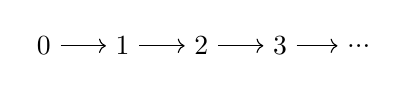
\begin{tikzpicture}[->]
			\node (0) {0};
			\node (1) [right of=0] {1};
			\node (2) [right of=1] {2};
			\node (3) [right of=2] {3};
			\node (4) [right of=3] {...};

			\path
			(0) edge node {} (1)
			(1) edge node {} (2)
			(2) edge node {} (3)
			(3) edge node {} (4);
		\end{tikzpicture}	
	\end{center}
\end{example}
\begin{example}
	il frame (S,R) dove \(S = \{2,3,4,5,6\}\) e \(R=\{(x,y) \in S \times S : x \text{ divide } y \}\)\\
	è rappresentato dal seguente grafo diretto:
	\begin{center}
		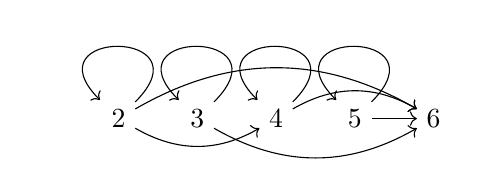
\begin{tikzpicture}[->]
			\node (2) {2};
			\node (3) [right of=2] {3};
			\node (4) [right of=3] {4};
			\node (5) [right of=4] {5};
			\node (6) [right of=5] {6};
  
			\path
			(2) edge[loop] node {} (2)
			(2) edge[bend right] node {} (4)
			(2) edge[bend left] node {} (6)
			(3) edge[loop] node {} (3)
			(3) edge[bend right] node {} (6)
			(4) edge[loop] node {} (4)
			(4) edge[bend left] node {} (6)
			(5) edge[loop] node {} (5)
			(5) edge node {} (6);
			(6) edge[loop] node {} (6)
		\end{tikzpicture}
	\end{center}
\end{example}
\begin{example}
	Il frame \((\{1,2,3\}, R)\) dove \(R = \{(x,y) \in \{1,2,3\} \times \{1,2,3\} : y=f(x)\}\)\\
	essedo \(f : \{1,2,3\} \rightarrow \{1,2,3\}\) la funzione definita da \(f(1) = 2, f(2) = 3, f(3) = 1\)\\
	è 
	\begin{center}
		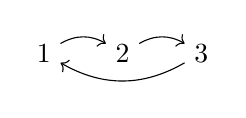
\begin{tikzpicture}[->]
			\node (1) {1};
			\node (2) [right of=1] {2};
			\node (3) [right of=2] {3};
  
			\path
			(1) edge[bend left] node {} (2)
			(2) edge[bend left] node {} (3)
			(3) edge[bend left] node {} (1);
		\end{tikzpicture}
	\end{center}
\end{example}
\begin{definition}
	un \textbf{modello} su un frame \((S,R)\) è una terna \((S,R,V)\)\\
	dove \(V : Var \rightarrow \mathcal{P}(S) \), ci dice in quali mondi le variabili valgono 1\\
	è detta \textbf{funzione di valutazione}.
\end{definition}
\begin{definition}
	una formula \(F\) si dice \textbf{Vera in un mondo x del modello M}\\
	e scriviamo \textbf{M \(\vDash_x\) F} se e solo se:
	\begin{enumerate}
		\item \underline{F è una variabile}: \(M \vDash_x F\) significa che \(x \in V(F)\)
		\item \underline{ F è \(\neg y\) e \(y\) è una variabile}: \(M \vDash_x F\) significa che \(x \notin V(y)\)
		\item \underline{F è del tipo \(\neg G\)}, dove \(G\) è una formula: \(M \vDash_x F\) significa che \(M \nvDash_x G\)
		\item \underline{F è del tipo \(G_1 \land G_2\)}: \(M \vdash_x F\) significa che \(M \vdash_x G_1\) e \(M \vDash_x G_2\)
		\item \underline{F è del tipo \(G_1 \lor G_2\)}: \(M \vdash_x F\) significa che \(M \vdash_x G_1\) o \(M \vDash_x G_2\)
		\item \underline{F è del tipo \(\Box G\)}: \(M \vDash_x F\) significa che \(M \vDash_y G\), per ogni \(y \in S : (x,y) \in R\),\\
				ossia per ogni mondo y raggiungibile da x.
		\item \underline{F è del tipo \(\diamond G\)}: \(M \vDash_x F\) significa che \(M \vDash_y G\) per qualche \(y \in S : (x,y) \in R\),\\
				ossia per almeno un mondo raggiungibile da x.
	\end{enumerate} 
\end{definition}
\begin{definition}
	una foruma F è \textbf{soddisfacibile} se esiste un modello\\
	\(M = (S, R, V)\) e un mondo \(x \in S\), tali che \(M \vDash_x F\).
\end{definition}
\begin{teorema}
	se una formula modale F è soddisfacibile,\\
	allora è soddisfacibile in una struttura di Kripke (S,R) tale che \(|S| \leq 2^{|F|}\),\\
	\(|F| = \)"lunghezza di F".\\
	Quindi il problema di soddisfacibilità di una formula modale è decidibile.\\
\end{teorema}

Se come frame prendiamo \(({0},R)\) dove \(R \subseteq S \times S = \{(0,0)\}\) è quindi \(S\) stesso,\\
una funzione di valutazione è \(V : Var \rightarrow \mathcal{P}(S) = \{\emptyset, \{0\}\} \simeq \{0,1\}\).\\
In questo modo i connettivi modali diventano superflui eritroviamo la logica modale che abbiamo già studiato.\\
La veritò di una formula del linguaggio della logica modale dipenderà quindi dal frame scelto, in particolare\\
dalla relazione R.
Ad esempio nella logica della necessità vogliamo che sia sempre vera la formula
\begin{center}
	\(\Box x \implies x\)\\
	"è necessaria che x, allora x"
\end{center}
Nella logica deontica la stessa formula la leggiamo "è obbligatorio che x, allora x"\\
e non vogliamo che questa affermazione sia sempre vera.\\
Perchè sia sempre vera la formula \(\Box x \implies x\), la relazione R del frame deve essere riflessiva,\\
ossia \((y,y) \in R \forall y \in S\).\\
Infatti, se R non fosse riflessiva ci sarebbe un mondo \(y \in S\) tale che \((y,y) \notin R\).\\
Sia \(Z = V(x), Z \subseteq S,\) tale che \(y \notin Z\) (cioè x è falsa nel mondo y).\\
Sia \(Z \supseteq \{z \in S : (y,z) \in R\}\) cioè x sia vera in tutti i mondi accessibili da y.\\
Allora se \(M = (S, R, V), M \vDash_y \Box x\) ma \(M \nvDash_y x\).\\
Nella logica Deeontica, dove non vogliamo che sia sempre vera la formula \(\Box x \implies x\),\\
non prenderemo una relazione riflessiva.\\
\begin{definition}
	una formula F si dice \textbf{Vera in un modello M}, scritto \textbf{\(M \vDash F\)}, se \(M \vDash_x F, \forall x \in S\),\\
	ossia se è vera in tutti i mondi di S.\\
\end{definition}
\begin{definition}
	Una formula si dice \textbf{valida in un frame (S,R)}, scritto \textbf{\((S,R) \vDash F\)},\\
	se è vera in tutti i modelli costruiti su (S,R).\\
\end{definition}
\begin{example}
	La formula \(\Box x \implies x\) è valida solo nel frame (S,R) in cui R è riflessiva.
\end{example}
\begin{definition}
	una formula F è \textbf{valida} se e solo se è valida du ogni frame, e scriviamo \textbf{\(\vDash F\)}\\
\end{definition}
\begin{definition}
	uno \textbf{schema di formule} è una collezione di formule aventi tutte la stessa forma sintattica.\\
	ad esempio, con lo schema \(\Box x \implies x\) si intendono tutte le forume di questa forma, come\\
	\(\Box x \implies x\), x varuabile, o \(\Box (\neg \diamond \neg x) \implies \neg \diamond \neg x\).
\end{definition}
Le tautologie della logica proposizionale sono valide su ogni frame.\\
Vediamo ora che lo schema di formule \(\Box (A \implies B) \implies (\Box A \implies \Box B)\) \\
è valido su ogni frame.\\
Sia \(w \in S\) un mondo e M un modello su un frame \((S,R)\).\\
Sia \(M \vDash_w \Box (A \implies B)\) e \(M \vDash_w \Box A\).\\
(dobbiamo solo controllare che quando \(\Box ( A \implies B )\) è vera,\\
allora se è vera \(\Box A\), è vera \(\Box B\)).\\
\(M \vDash_w \Box (A \implies B)\) significa che \(M \vDash_v A \implies B, \forall v \in S t.c. (w,v) \in R\).\\
\(M \vDash_w \Box A\) significa che \(M \vDash_v A, \forall v \in S t.c. (w,v) \in R\).\\
Dunque \(M \vDash_v B, \forall v \in S t.c. (w,v) \in R\), ossia \(M \vDash_w \Box B\).\\
Abbiamo dimostrato che 
\begin{center}
	\(\vDash \Box (A \implies B) \implies (\Box A \implies \Box B)\)
\end{center}
chiameremo K tale schema.\\
Mostriamo che i seguenti schemi sono validi:
\begin{enumerate}
	\item \(\Box (A \land B) \iff (\Box A \land \Box B)\)
	\item \(\Diamond (A \lor B) \iff (\Diamond A \lor \Diamond B)\)
	\item \(\Box (A \implies B) \implies (\Diamond A \implies \Diamond B)\)
	\item \(\Diamond (A \implies B) \implies (\Box A \implies \Diamond B)\)
\end{enumerate}
\newpage
\begin{enumerate}
	\item \(M \vDash_w \Box (A \land B)\) se e solo se \(M \vDash_v A \land B, \forall v \in S t.c. (w,v) \in R\),\\
				se e solo se \(M \vDash_v A \text{ e } M \vDash_v B \forall v \in S t.c. (w,v) \in R\),\\
				se e solo se \(M \vDash_w \Box A\) e \(M \vDash_w \Box B\),\\
				se e solo se \(M \vDash_w (\Box A \land \Box B)\), dove M è un modello su un frame \((S,R)\) e \(w \in S\)
	\item \(M \vDash_w \Diamond (A \lor B)\) se e solo se \(M \vDash_v A \lor B, \exists v \in S t.c. (w,v) \in R\),\\
				se e solo se \(M \vDash_v A \text{ o } M \vDash_v B \exists v \in S t.c. (w,v) \in R\),\\
				se e solo se \(M \vDash_w \Diamond A \text{ o } M \vDash_w \Diamond B\),\\
				se e solo se \(M \vDash_w (\Diamond A \lor \Diamond B)\), dove M è un modello su un frame \((S,R)\) e \(w \in S\)
	\item \(M \vDash_w \Box (A \implies B)\) e \(M \vDash_w \Diamond A\) implicano che \(M \vDash_v (A \implies B), \forall v \in S t.c. (w,v) \in R\),\\
				e \(M \vDash_v A, \exists v \in S t.c. (w,v) \in R\).\\
				Quindi \(M \vDash_v B, \exists  v \in S t.c. (w,v) \in R\),\\
				ossia \(M \vDash_w \Diamond B\), dove M è un modello su un frame \((S,R)\) e \(w \in S\)
	\item \(M \vDash_w \Diamond (A \implies B)\) e \(M \vDash_w \Box A\) implicano che \(M \vDash_v (A \implies B), \exists v \in S t.c. (w,v) \in R\),\\
				e \(M \vDash_v A, \forall v \in S t.c. (w,v) \in R\).\\
				Quindi \(M \vDash_v B, \exists v \in S t.c. (w,v) \in R\),\\
				ossia \(M \vDash_w \Diamond B\), dove M è un modello su un frame \((S,R)\) e \(w \in S\)\\
\end{enumerate}
Abbiamo già mostrato che se M è un modello su un frame \((S,R)\) con \(R\) non riflessiva,\\
allora \(\Box x \implies x\) non è vera nel modello M. Quindi la formula \(\Box x \implies x\) non è valida.
\begin{center}
	\(\nvDash \Box x \implies x\)
\end{center}
Mostiamo che i seguenti schemi di fromule non sono validi:
\begin{enumerate}
	\item \(\Diamond A \implies \Box A\)
	\item \(\Box A \implies A\) (già visto)
	\item \(\Box A \implies \Box \Box A\)
	\item \(\Box (A \implies B) \implies (\Box A \implies \Diamond B)\)
	\item \(\Box (\Box A \implies B) \lor \Box (\Box B \implies A)\)
	\item \(\Box (A \lor B) \implies (\Box A \lor \Box B)\)
	\item \(\Box(\Box A \implies A) \implies \Box A\)
\end{enumerate}
\newpage
\begin{enumerate}
	\item \begin{tikzpicture}[->]
				\node (1) {1};
				\node (2) [right of=1] {2};
				\path
				(1) edge[loop] node {} (1)
				(1) edge node {} (2);
			\end{tikzpicture} \(M = (\{1,2\},\{(1,2),(1,1),\}, V)\)\\
			\(V(x) = 2 \) (ossia la formiula x è vera solo nel mondo 2)\\
			Quindi \(M \vDash_! \Diamond x\) e \(M \nvDash_1 \Box x\), \\
			ossia \(M \nvDash_1 (\Diamond x \implies \Box x)\)
	\item già gvisto.
	\item 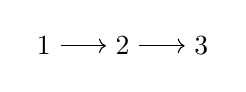
\begin{tikzpicture}[->]
				\node (1) {1};
				\node (2) [right of=1] {2};
				\node (3) [right of=2] {3};
				\path
				(1) edge node {} (2)
				(2) edge node {} (3);
			\end{tikzpicture} \(M = (\{1,2,3\},\{(1,2),(2,3)\}, V)\)\\
			\(V(x) = \{2\}\)\\
			Quindi \(M \vDash_1 \Box x\). Abbiamo che \(M \vDash_1 \Box \Box x\) se e solo se \(M \vDash_2 \Box x\),\\
			se e solo se \(M \vDash_3 x\), ma \(M \nvDash_3 x\), quindi \(M \nvDash_1 \Box \Box x\)
	\item \begin{tikzpicture}[->]
				\node (1) {1};
				\node (2) [right of=1] {2};
				\path
				(1) edge node {} (2);
			\end{tikzpicture} \(M = (\{1,2\}, V)\)\\
			\(V(x) = \{1\}\)\\
			\(M \vDash_2 \Box (A \implies B)\), \(M \vDash_2 \Box A\),\\
			ma \(M \nvDash_2 \Diamond B\), perchè non esiste \(v \in \{1,2\} t.c M \vDash_v , (2,v) \in R\)
	\item prendiamo \(A = B = x\) nel frame 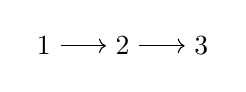
\begin{tikzpicture}[->]
				\node (1) {1};
				\node (2) [right of=1] {2};
				\node (3) [right of=2] {3};
				\path
				(1) edge node {} (2)
				(2) edge node {} (3);
			\end{tikzpicture} \(M = (\{1,2,3\},\{(1,2),(2,3)\}, V)\)\\
			\(V(x) = \{3\}\), si ha\\
			\(M \vDash_1 \Box (\Box x \implies x)\) se e solo se \(M \vDash_2 \Box x \implies x\),\\
			se e solo se \(M \vDash_3 x\) e \(M \nvDash_2 x\), ma \(M \nvDash_2 \Box x\),\\
			quindi \(M \nvDash_1 \Box (\Box x \implies x)\)
	\item \begin{tikzpicture}[->]
			\node (1) {1};
			\node (2) [right of=1] {2};
			\path
			(1) edge[loop] node {} (1)
			(1) edge node {} (2);
		\end{tikzpicture} \(M = (\{1,2\},\{(1,2),(1,1),\}, V)\)\\
		\(V(x) = \{1\}, V(y) = \{2\}\)\\
		\(M \vDash_1 \Box (x \lor y)\) se e solo se \(M \nvDash_1 (x \lor y)\) e \(M \nvDash_2 (x \lor y)\).\\
		Quindi abbiamo che \(M \nvDash_1 \Box (x \lor y)\).\\
		invece \(M \vDash_1 (\Box x \lor \Box y)\) se e solo se \(M \vDash_1 x\) e \(M \vDash_2 x\) o \(M \vDash_1 y\) e \(M \vDash_2 y\),\\
		Dunque \(M \nvDash_1 (\Box x \lor \Box y)\)
	\item \begin{tikzpicture}[->]
				\node (1) {1};
				\node (2) [right of=1] {2};
				\node (3) [right of=2] {3};
				\path
				(1) edge[loop] node {} (1)
				(1) edge node {} (2)
				(2) edge node {} (3);
			\end{tikzpicture} \(M = (\{1,2,3\},\{(1,2),(2,3)\}, V)\)\\
			\(V(x) = \{2,3\}\)\\
			\(M \vDash_1 \Box (\Box x \implies x)\) se e solo se \(M \vDash_1 (\Box x \implies x)\) e \(M \vDash_2 (\Box x \implies x)\),\\
			che sono entrambe vere, quindi \(M \vDash_1 \Box (\Box x \implies x)\)\\
			invece \(M \nvDash_1 \Box x\) perchè \(M \nvDash_1 x\).
\end{enumerate}
\newpage
\subsection{corrispondenza e non esprimibilità}
\begin{definition}
	diciamo che un frame (S,R) gode di una certa proprietà se ne gode\\
	la relazione R. In molti casi una proprietà di un frame equivale alla validità\\
	di uno schema di formule modali nei frame con quella proprietà.\\
\end{definition}
\begin{teorema}
	Lo schema \(\Box A \implies A\) è valido in un frame (S,R) se e solo se R è riflessiva.
\end{teorema}
\begin{dimostrazione}
	Già visto.
\end{dimostrazione}
\begin{teorema}
	Lo schema \( A \implies \Box \Diamond A\) è valido in un frame (S,R) se e solo se R è simmetrica.
\end{teorema}
\begin{dimostrazione}
	Sia R simmetrica, ossia \((x,y) \in R \implies (y,x) \in R\).\\
	Sia \(M \vDash_w A\) e \((w,v) \in R\). Dunque \((v,w) \in R\) e \(M \vDash_v \Diamond A \forall v \in S t.c. (w,v) \in R\),\\
	Ossia \(M \vDash_w \Box \Diamond A\).\\
	Adesso assumiamo che lo schema \(A \implies \Box \Diamond A \) sia valido in (S,R).\\
	Sia x una variabile e \(V(x) = \{s\}\);\\
	sia \(t \in S t.c. (s,t) \in R\). Quindi \(M \vDash_s x\).\\
	Dalla calidità dello schema segue allora che \(M \vDash_s \Box \Diamond x\),\\
	Da cui \(M \vDash_t \Diamond x\). Quindi esiste \(r \in S t.c. (t,r) \in R e M \vDash_r x\),\\
	ossia \(r = s\)
\end{dimostrazione}
\begin{teorema}
	Lo schema \(\Box A \implies \Box \Box A\) è valido in un frame (S,R)\\
	 se e solo se R è transitiva.
\end{teorema}
\begin{dimostrazione}
	Sia R transitiva, ossia \((x,y) \in R, (y,z) \in R \implies (x,z) \in R\).\\
	Sia \(M \vDash_w \Box A\), ossia \(M \vDash_v A \forall v \in S t.c. (w,v) \in R\).\\
	Sia \(u \in S t.c. (v,u) \in R\), con \((w,v) \in R\).\\
	Allora \((w,u) \in R\) e quindi \(M \vDash_v \Box A, \forall v \in S t.c. (w,v) \in R\),\\
	Ossia \(M \vDash_w \Box \Box A\).\\
	Assumiamo adesso che sia valido lo schema \(\Box A \implies \Box \Box A\) su un frame (S,R).\\
	Sia x una variabile, \(s \in S\) e \(V(x) = \{w \in S : (s,w) \in R\}\).\\
	Allora \(M \vDash_s \Box x\) e quindi per la validità dello schema, \(M \vDash_s \Box \Box x \),\\
	Da cui \(M \vDash_t \Box x \forall t \in S t.c. (s,t) \in R\),\\
	ossia \(M \vDash_r x \forall r \in S t.c. (t,r) \in R\), \((s,t) \in R\).\\
	da ciò segue che \(r \in V(x)\) ossia \((s,t) \in R\) e \((t,r) \in R \implies (s,r) \in R\)\\
\end{dimostrazione}
Adesso vediamo che ci sono anche proprietà dei frame non esprimibili in termini di validità di schemi di formule modali.\\
\newpage
\subsection{Morfismi di modelli}
\begin{definition}
	Siano \((S_1, R_1)\) e \((S_2, R_2)\) due frame.\\
	una funziuone \(f : S_1 \rightarrow S_2\) è un \textbf{morfismo di frame} se:
	\begin{center}
		\((x,y)\in R_1 \implies (f(x), f(y)) \in R_2, \forall x,y \in S_1\)
	\end{center}
\end{definition}
\begin{example}
	siano \((\mathbb{N}, R_1)\) e \((\mathbb{N}, R_2)\) i frame tali che
	\begin{center}
		\(R_1 = R_2 = \{(x,y) \in \mathbb{N} \times \mathbb{N} : x < y\}\)
	\end{center}
	allora la funzione \(f : \mathbb{N} \rightarrow \mathbb{N}\) definita da \(f(n) = n^2\) è un morfismo di frame.
\end{example}
\begin{example}
	siano \((\mathbb{N}, R_1)\) e \((\mathbb{N}, R_2)\) i frame tali che
	\begin{center}
		\(R_1 = R_2 = \{(x,y) \in \mathbb{N} \times \mathbb{N} : x \text{ divide } y\}\)\\
	\end{center}
	allora la funzione \(f : \mathbb{N} \rightarrow \mathbb{N}\) definita da \(f(n) = n + 1 \) non è un morfismo di frame.
\end{example}
\begin{definition}
	siano \(M_1 = (S_1, R_1, V_1)\) e \(M_2 = (S_2, R_2, V_2)\) due modelli.\\
	Un morfismo di fame \(f: (S_1, R_1) \rightarrow (S_2, R_2)\) è un \textbf{morfismo di modelli} se:
\end{definition}
\begin{enumerate}
	\item \(w \in V_1(x) \iff f(w) \in V_2(x), \forall w \in S_1, x \in Var\)
	\item \((f(w),y) \in R_2 \implies \exists v \in S_1 t.c. (w,v) \in R_1, f(v) = y, \forall w \in S_1, y \in S_2\)
\end{enumerate}
\textbf{Nota:} I morfismi di modelli sono solitamente detti \textbf{p-morfismi}.\\
\begin{example}
	Siano \(M_1 = (\mathbb{N}, R_1, V_1)\) e \(M_2 = (\{0,1\}, \{0,1\} \times \{0,1\}, V_2)\)\\
	dove \(R_1 = \{(x,y) \in \mathbb{N} \times \mathbb{N} : x \leq y\}\),\\
	\(Var = \{x\}\) e \(V_1(x)= \{2n : n \in \mathbb{N}\}, V_2(x) = \{0\}\).\\
	Sia \(f: \mathbb{N} \rightarrow \{0,1\}\) definita da \(f(n) = n \mod 2\).\\
	Allora \(f\) è un morfismo di modelli, infatti:
	\begin{enumerate}
		\item \(x \leq y \implies (x \mod 2, y \mod 2) \in \{0,1\} \times \{0,1\}\)
		\item \(w \in V_1(x) \iff w \in \{2n: n \in \mathbb{N}\}\); allora\\
				\(w \in V_1(x) \implies f(w) = 0\).\\
				\(f(w) \in V_2(x) \iff f(w) = 0 \); allora \(f(w) \in V_2(x) \implies w \in V_1(x)\)
		\item \((f(w),y) \in R_2 = \{0,1\} \times \{0,1\}\):
				\begin{enumerate}
					\item \(f(w) = 0\): se \(y=0\) allora \(w \leq w\) e \(f(w) = 0 = y\).\\
							Se \(y=1\) allora \(w \leq w+1\) e \(f(w+1) = 1 = y\).
					\item \(f(w) = 1\): se \(y=0\) allora \(w \leq w + 1\) e \(f(w + 1) = 0 = y\).\\
							Se \(y=1\) allora \(w \leq w\) e \(f(w) = 1 = y\).\\
				\end{enumerate}
	\end{enumerate}
\end{example}
\newpage
\textbf{Lemma 1:} sia \(f: (S_1, R_1, V_1) \rightarrow (S_2, R_2, V_2)\)\\
un morfismo dal modello \(M_1\) al modello \(M_2\). Allora
\begin{center}
	\(M_1 \vDash_w F \iff M_2 \vDash_{f(x)} F, \text{ se e solo se } w \in S_1\) e ogni  formula \(F\)
\end{center}
\begin{dimostrazione}
	se \(F\) è una variabile allora \(M_1 \vDash_w F \text{ se e solo se } w \in V_1(F)\\
	\text{se e solo se } f(w) \in V_2(F)\) (per il punto 1 nella definizone di morfismo di modelli)\\
	se e solo se \(M_2 \vDash_{f(w)} F\).\\
	per tutti gli altri tipi di formule, si dimostra induttivamente sulla costruzione della formula.\\
	vediamo dsolo il caso in cui \(F = \Diamond G\).\\
	Sia \(M_1 \vDash_w \Diamond G\), allora esiste \(v \in S_1 t.c. (w,v) \in R_1\) e \(M_1 \vDash_v G\).\\
	Poiché \((f(w),f(v)) \in R_2\) perchè \(f\) è un morfismo di modelli e induttivamente \(M_2 \vDash_{f(v)} G\),\\
	allora \(M_2 \vDash_{f(w)} \Diamond G\).\\
	Sia ora \(M_2 \vDash_{f(w)} \Diamond G\), allora esiste \(u \in R_2 t.c. (f(w),u) \in R_2\) e \(M_2 \vDash_u G\).\\
	Per la condizione 2 nella definizione di morfismo di modelli, \\
	esiste \(v \in S_1 t.c. (w,v) \in R_1\) e \(f(v) = u\).\\
	Per ipotesi induttiva \(M_1 \vDash_v G\), e quindi \(M_1 \vDash_w \Diamond G\).
\end{dimostrazione}
\textbf{Lemma 2:} sia \(f: (S_1,R_1,V_1) \rightarrow (S_2,R_2,V_2)\)\\
un morfismo dal modello \(M_1\) al modello \(M_2\). se \(f\) è suriettiva, allora
\begin{center}
	\(M_1 \vDash F \text{ se e solo se } M_2 \vDash F, \forall F\)
\end{center}
per ogni formula F.
\begin{dimostrazione}
	\(M_1 \vDash F\) se e solo se \(M_1 \vDash_w F, \forall w \in S_1\).\\
	se e solo se \(M_2 \vDash_{f(w)} F, \forall w \in S_1\) (per il lemma 1).\\
	se e solo se \(M_2 \vDash F\), perchè \(f\) è suriettivo.
\end{dimostrazione}
\textbf{Lemma 3:} sia \(M_2\) un modello su \(S_2, R_2\) e \(f: (s_1,R_1) \rightarrow (S_2, R_2)\)\\
un morfismo di frame tale che valga la condizione 2 della definizione di morfismo di modelli.\\
Allora esiste un modello \(M_1\) su \(S_1, R_1\) tale che \(f: M_1 \rightarrow M_2\)\\
è un morfismo di modelli.
\begin{dimostrazione}
	Basta definire \(M_1 = (S_1, R_1, V_1)\)\\
	con \(V_1(x) = \{ w \in S_1 : M_2 \vDash_{f(w)} x\} \forall x \in Var\).
\end{dimostrazione}
\textbf{Lemma 4:} sia \(f: (S_1, R_1) \rightarrow (S_2, R_2)\) un morfismo di frame\\
tale che valga la condizione 2 della definizione di morfismo di modelli.\\
Se \(f\) è suriettivo, si ha \((S_1, R_1) \vDash F \implies (S_2, R_2) \vDash F\),\\
per ogni formula F.
\begin{dimostrazione}
	sia \(S_2, R_2 \nvDash F\). Allora esisite un modello \(M_2\) su \((S_2, R_2)\)\\
	tale che \(M_2 \nvDash F\). Per il lemma 3 esiste un modello \(M_1\) su \((S_1, R_1)\)\\
	tale che \(f: M_1 \rightarrow M_2\) è un morfismo di modelli.\\
	Dato che \(f\) è suriettivo, per il lemma 2 si ha \(M_1 \nvDash F\),\\
	ossia \((S_1, R_1) \nvDash F\).\\
\end{dimostrazione}
\newpage
\begin{definition}
	Una relazione \(R\) su un insieme \(X\) si dice \textbf{antisimmetrica} se
	\begin{center}
		\((x,y) \in R, (y,x) \in R \implies x = y, \forall x,y \in X\)
	\end{center}
\end{definition}
\begin{example}
	L'ordinamento \(\leq\) dei numeri naturali è una relazione antisimmetrica su \(\mathbb{N}\).
\end{example}
\begin{example}
	La relazione \(x | y\) su \(\mathbb{N}\) è antisimmetrica.
\end{example}
\begin{example}
	La relazione \(A \subseteq B\) su \(\mathcal{P}(X)\) di un insieme \(X\) è antisimmetrica.
\end{example}
\begin{teorema}
	L'antisimmetria non è esprimibile,\\
	ossia non esiste una formula \(F\) tale che \((S,R) \vDash F\) se e solo se \(R\) è antisimmetrica.
\end{teorema}
\begin{dimostrazione}
	sia \((S_1,R_1) = (\mathbb{N},\leq)\) e \((S_2, R_2) = (\{0,1\}, \{0,1\} \times \{0,1\})\).\\
	Nell'esempio di morfismo di modelli abbiamo visto che la funzione \(f: \mathbb{N} \rightarrow \{0,1\}\) definita da\\
	\(f(n) = n \mod 2\) è un morfismo dal frame \((\mathbb{N},\leq)\) al frame \((\{0,1\}, \{0,1\} \times \{0,1\})\)\\
	che soffisfa la condizione 2 della definizione di morfismo di modelli.\\
	La relazione \(\leq\) su \(\mathbb{N}\) è antisimmetrica.\\
	supponiamo per assurdo che esista una formula \(F\) come nell'enunciato del teorema.\\
	allora \((\mathbb{N},\leq) \vDash F\).\\
	per il lemma 4 si ha che \((\{0,1\}, \{0,1\} \times \{0,1\}) \vDash F\).\\
	da cui seguirebbe che \(R_2\) è antisimmetrica, ma non è vero.
\end{dimostrazione}
\newpage
\subsection{Logiche modali normali}
Abbiamo già mostrato che lo schema di formule
\begin{center}
	\(K: \Box (A \implies B) \implies (\Box A \implies \Box B)\)
\end{center}
è valido, \(\vDash K\).\\
Adesso viediamo che lo schema di formule
\begin{center}
	\(def_\Diamond : \Diamond A \iff \neg \Box \neg A\)
\end{center}
è valido, \(\vDash def_\Diamond\).\\
\begin{dimostrazione}
	Sia \((S,R)\) un frame, \(M\) un modello su \((S,R)\) e \(w \in S\).\\
	Allora \(M \vDash_w \Diamond A\) se e solo se esiste \(v \in S t.c. (w,v) \in R\) e \(M \vDash_v A\).\\
	\(M \vDash_w \neg \Box \neg A\) se e solo se \(M \nvDash_w \Box \neg A\),\\
	se e solo se esiste \(v \in S t.c. (w,v) \in R\) e \(M \nvDash_v \neg A\),\\
	se e solo se esite \(v \in S t.c. (w,v) \in R\) e \(M \vDash_v A\).\\
	abbiamo quindi dimostrato che \(\vDash def_\Diamond\)
\end{dimostrazione}
\begin{definition}[Sostituzione uniforme]
	Sia \(x\) una variabile e \(F\) una formula.\\
	Definiamo l'operzione di sostituzione uniforme di \(F\) al posto di \(x\) in una formula \(G\),\\
	indicato come
	\begin{center}
		\(G[F/x]\)
	\end{center}
	La formula ottenuta da \(G\) dove ogni occorrenza di \(x\) è stata sostituita con \(F\).
\end{definition}
\begin{example}
	Sia \(G\) la formula \(\Box x \implies x \land y\) e \(F\) la formula \(\Diamond y \iff \neg \Box \neg y\).\\
	Allora \(G[F/x] = \Box (\Diamond y \iff \neg \Box \neg y) \implies (\Diamond y \iff \neg \Box \neg y) \land y\)
\end{example}
\begin{definition}
	Una \textbf{logica modale normale} è un insieme \(\Gamma\) di formule tale che:
	\begin{enumerate}
		\item \(\Gamma\) contiene tutte le tautologie della logica proposizionale
		\item \(\Gamma\) contiene tutte le istanze dello schema \(K: \Box (A \implies B) \implies (\Box A \implies \Box B)\)
		\item \(\Gamma\) contiene tutte le istanze dello schema \(def_\Diamond : \Diamond A \iff \neg \Box \neg A\)
		\item \(\Gamma\) è chiuso sotto \textbf{modus ponens}:\\
				se \(A \in \Gamma\) e \((A \implies B) \in \Gamma\), allora \(B \in \Gamma\)
		\item \(\Gamma\) è chiuso sotto \textbf{necessitazione}:\\
				se \(A \in \Gamma\), allora \(\Box A \in \Gamma\)
		\item \(\Gamma\) è chiuso sotto \textbf{sostituzione uniforme}:\\
				se \(A \in \Gamma\), allora \(A[B/x] \in \Gamma\)
	\end{enumerate}
\end{definition}
\begin{example}
	se \((S,R)\) è un frame, \(\{F: (S,R) \vDash F\}\) è una logica normale.
\end{example}
\begin{example}
	\(\{F: \vDash F\}\) è una logica normale.
\end{example}
\begin{example}
	se \(M\) è un modello su un frame \((S,R)\), \(\{F: M \vDash F\}\) NON è una logica normale.
\end{example}
per verificare queste affermzioni vedere sezione 1.4 del libro\\
\textit{"Corso di logica modale proposizionale"} di E. Orlandelli e G. Corsi.\\
\newpage
\begin{definition}
	La \underline{logica modale K} è definita dai seguenti schemi di assioni e regole:
	\begin{enumerate}
		\item schemi di assiomi:
				\begin{enumerate}
					\item tutte le tautologie della logica proposizionale
					\item \(K: \Box (A \implies B) \implies (\Box A \implies \Box B)\)
					\item \(def_\Diamond : \Diamond A \iff \neg \Box \neg A\)
				\end{enumerate}
		\item regole di inferenza:
				\begin{enumerate}
					\item modus ponens
					\item necessitazione
					\item sostituzione uniforme
				\end{enumerate}
	\end{enumerate}
\end{definition}
\begin{definition}
	Data una logica modale L\\
	una \textbf{dimostrazione in L} è una successione finita di formule tali che ognuna di esse\\
	o è un assioma o è ottenuta da formule precedenti tramite una regola di inferenza
\end{definition}
\begin{definition}
	una formula \(F\) si dice \textbf{Teorema di L}, scritto \textbf{\(\vdash_L F\)}\\
	se e solo se esite una dimostrazione in \(L\) in cui la ultima formula è \(F\)
\end{definition}
\begin{example}
	\(\Box (A \land B) \implies \Box A\) è un teorema della logica K:
	\begin{enumerate}
		\item \(\vdash_K A \land B \implies A\) (Tautologia)
		\item \(\vdash_K \Box (A \land B \implies A)\) (Necessitazione)
		\item \(\vdash_K \Box (A \land B \implies A ) \implies (\Box (A \land B ) \implies \Box A)\) (K)
		\item \(\vdash_K \Box (A \land B ) \implies \Box A\) (Modus Ponens)
	\end{enumerate}
\end{example}
\begin{teorema}
	L'insieme \(\{F : \vdash_K F\}\) è chiuso sotto sostituzione uniforme.\\
\end{teorema}
\begin{dimostrazione}
	Vedi teorema 3.5 del libro \textit{"Corso di logica modale proposizionale"} di E. Orlandelli e G. Corsi.
\end{dimostrazione}
\newpage
Nelle logiche Epistemiche si estende la logica K aggiungendo lo schema di assimi
\begin{center}
	\(\Box F \implies F\)\\
	(se si sa che \(F\), allora \(F\) vale)
\end{center}
che, come abbiamo visto, non vogliamo come assioma in una logica Deontica\\
(se \(F\) è obbligatorio non è detto che \(F\) valga).
\begin{list}{-}{}
	\item La logica K a cui aggiungiamo l'assioma \(\Box F \implies F\) si chiama \underline{logica T}.\\
			dato lo schema di formule \(\Box F \implies F\),\\
			i teoremi della logica T sono validi su frame riflessivi.
	\item se accettiamo il \textbf{principio di introspezione epistemica positiva}, ossia se assumiamo che\\
			Ogni volta che si sa qualcosa si sa di saperla, aggiungiamo l'assioma \(\Box F \implies \Box \Box F\).\\
			Avremmo così definito la logica \underline{S4}.\\
			I teoremi della logica S4 sono validi su frame riflessivi e transitivi, perchè lo schema di formule \(\Box F \implies \Box \Box F\) esprtime la transitività.
	\item se accettiamo anche il \textbf{principio di introspezione epistemica negativa}, ossia se ogni volta che\\
			non si sa qualcosa si sa di non saperla, aggiungiamo l'assioma \(\neg \Box F \implies \Box \neg \Box F\).\\
			Avremmo così definito la logica \underline{S5}.\\
			I teoremi della logica S5 sono validi su frame riflessivi, transitivi e simmetrici ossia sulle relazioni di equivalenza.
\end{list}
Dobbiamo solo far vedere la validità suiframe simmetrici.\\
deriviamo lo schema di formule \(F \implies \Box \Diamond F\) da S5:
\begin{enumerate}
	\item \(\vdash_{S5} \neg \Box \neg F \implies \Box \neg \Box \neg F\)
	\item \(\vdash_{S5} \Diamond F \implies \Box \Diamond F\) (1 + \(def_\Diamond\))
	\item \(\vdash_{S5} \Box \neg F \implies \neg F\) (assioma T)
	\item \(\vdash_{S5} \neg \neg F \implies \neg \Box \neg F\) (3 + tautologia)
	\item \(\vdash_{S5} F \implies \Diamond F\) (4 + \(def_\Diamond\) + tautologia)
	\item \(\vdash_{S5} F \implies \Box \Diamond F\) (transitività implicazione + 5 + 2)
\end{enumerate}
Quindi \(F \implies \Box \Diamond F\) è un teorema di S5.\\
\newpage
Adesso facciamo vedere che \(\neg \Box F \implies \Box \neg \Box F\)\\
è un teorema di K + 1. 2. 3. :
\begin{enumerate}
	\item \(\Box F \implies F\)
	\item \(\Box F \implies \Box \Box F\)
	\item \(F \implies \Box \Diamond F\)
	\item \(\vdash \Box \Box F \iff \Box F\) (1 e 2)
	\item \(\vdash \neg \Box \neg \neg \Box \neg F \implies \neg \Box \neg F\) (4 + tautologia)
	\item \(\vdash \Diamond \Diamond F \implies \Diamond F\) (\(def_\Diamond\))
	\item \(\vdash \Diamond F \implies \Box \Diamond \Diamond F\) (3)
	\item \(\vdash \Box(\Diamond \Diamond F \implies \Diamond F)\) (6 + necessitazione)
	\item \(\vdash \Box \Diamond \Diamond F \implies \Box \Diamond F\) (schema K + modus ponens)
	\item \(\vdash \Diamond F \implies \Box \Diamond F\) (7 + 9)
	\item \(\vdash \neg \Box \neg F \implies \Box \neg \Box \neg F\) (\(def_\Diamond\))
	\item \(\vdash \neg \Box F \implies \Box \neg \Box F\) (tautologia)
\end{enumerate}
Quindi la logica basata su principi episistemici che abbiamo considerato ragionevoli\\
si supporta su frame che sono relazioni di equivalenza.\\
\begin{definition}
	una logica L è \textbf{valida (sound)} se \(\vdash_L A \implies \vDash A\)
\end{definition}
\begin{teorema}
	La logica K è valida.
\end{teorema}
\begin{dimostrazione}
	Sia \(B_1,B_2,...,B_n\) una dimaostrazione di A in K, con \(B_n \equiv A\).\\
	\(B_1\) è valida perchè è un assioma.\\
	se \(i > 1\), allora \(B_i\) è un assioma o è ottenuta da formule precedenti\\
	tramite necessitazione o modus ponens.
	\begin{enumerate}
		\item \(\vdash_K B_j\), per induzione \(\vDash B_j\) e allora \(\vDash \Box B_j\), quindi \(B_i = \Box B_j\) è valida.
		\item \(\vdash_K B_j, \vdash_K B_h\) dove \(B_h \equiv B_i \implies B_i\). Allora per induzione \(\vDash B_j, \vDash B_j \implies B_i\)\\
				e quindi \(\vDash B_i\)
	\end{enumerate}
\end{dimostrazione}
\begin{definition}
	una logica L è \textbf{completa} se \(\vDash A \implies \vdash_L A\)
\end{definition}
\begin{teorema}
	La logica K è completa.
\end{teorema}
\begin{dimostrazione}
	vedi capitolo 4 del libro \textit{"Corso di logica modale proposizionale"} di E. Orlandelli e G. Corsi.
\end{dimostrazione}
\newpage
\subsection{Logiche multimodali e connettivi modali n-ari}
Finora abbiamo studiato logiche modali con un solo connettivo modale 1-ario, \(\Box\).\\
(come abbiamo visto, l'altro connettivo modale, \(\Diamond\) può essere definito usando \(\Box\)).\\
Il connettivo \(\Box\) era 1-ario nel senso che si applicava ad una sola formula.\\
Adesso consideriamo Logiche modali con più di un connettivo modale,
\begin{center}
	\(\Box_1, \Box_2, ...\)\\
\end{center}
e connettivi modali n-ari ossia
\begin{center}
	\(\Box (F_1, F_2, ..., F_n)\) dove \(F_i\) sono formule.\\
\end{center}
Vediamo qual'è la semantica dei connettivi modali n-ari.\\
Sia S un insieme, \(R \subseteq S \times ... \times S\), (\(n + 1\) volte)\\
Una relazione \((n + 1)\)-aria su S e \(M\) un modello su \(S,R\).\\
sia \(w \in S\), scriviamo
\begin{center}
	\(M \vDash_w \Box (F_1, F_2, ..., F_n)\)
\end{center}
se e solo se \(\forall v_1 \in S, ... , v_n \in S\) tali che \((w,v_1,...,v_n) \in R\), si ha \(M \vDash_{v_1} F_1, ... , M \vDash_{v_n} F_n\).\\
\subsubsection{logiche temporali LTL (linear-time temporal logic)}
Queste logiche hanno tre connettivi modali 1-ari:
\begin{center}
	\(X, F, G\)
\end{center}
\(X\) significa "neXt state" (anche indicato con "O")\\
\(F\) significa "some Future state"\\
\(G\) significa "all future states (Globally)"\\
e tre connettivi modali 2-ari:
\begin{center}
	\(U, W, R\)
\end{center}
\(U\) significa "Until"\\
\(W\) significa "Weak-until"\\
\(R\) significa "Release"\\
\newpage
\textbf{Semantica:}\\
Sia S un insieme, \(R \subseteq S \times S\) e \(M\) un frame tale che \(R\) \underline{non è riflessiva}.\\
con \(R^*\) indichiamo la \underline{chiusura riflessiva e transitiva} di \(R\),\\
ossia ogni volta che in \(R\) abbiamo
\begin{center}
	\begin{tikzpicture}[->]
		\node (1) {x};
		\node (2) [right of=1] {y};
		\node (3) [right of=2] {z};
		\path
		(1) edge node {} (2)
		(2) edge node {} (3);
	\end{tikzpicture}
\end{center}
in \(R^*\) abbiamo
\begin{center}
	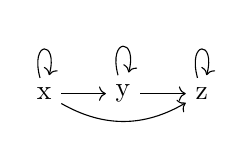
\begin{tikzpicture}[->]
		\node (1) {x};
		\node (2) [right of=1] {y};
		\node (3) [right of=2] {z};
		\path
		(1) edge node {} (2)
		(1) edge [bend right] node {} (3)
		(2) edge node {} (3)
		(1) edge [loop above] node {} (1)
		(2) edge [loop above] node {} (2)
		(3) edge [loop above] node {} (3);
	\end{tikzpicture}
\end{center}
\begin{enumerate}
	\item X è da considerare come \(\Box\) sul frame \((S,R)\)
	\item G è da considerare come \(\Box\) sul frame \((S,R^*)\)
	\item F è da considerare come \(\Diamond\) sul frame \((S,R^*)\),\\
			quindi \(F \varphi = \neg G \neg \varphi\) per ogni formula \(\varphi\)
	\item U è un connettivo modale 2-ario. è definito da
			\(M \vDash_x U(\varphi, \psi)\) se e solo Se
			\begin{enumerate}
				\item \(\exists z \in S t.c. (x,z) \in R^*\) e \(M \vDash_z \psi\)
				\item \(M \vDash_y \varphi \forall y \in S t.c. (x,y) \in R^*, (y,z) \in R^*, y \neq z\)
			\end{enumerate}
	\item \(W(\varphi, \psi)\) se e solo se \(U(\varphi, \psi)\) oppure \(G \varphi\)
	\item \(R(\varphi, \psi)\) se e solo se \(\neg U(\neg \varphi, \neg \psi)\)
\end{enumerate}
Quindi gli unici connettivi modali per definire questa logica solo \(X, G\) e \(U\).\\
Gli altri sono esprimibili in termini di questi.
\begin{example}
consideriamo la relazione:
	\begin{center}
		\((S,R)\) :
		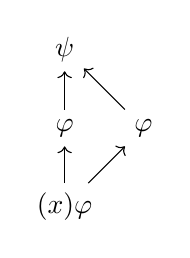
\begin{tikzpicture}[->]
			\node (1) {\((x) \varphi\)};
			\node (2) [above of = 1] {\(\varphi\)};
			\node (3) [right of=2] {\(\varphi\)};
			\node (4) [above of =2] {\(\psi\)};
			\path
			(1) edge node {} (2)
			(1) edge node {} (3)
			(2) edge node {} (4)
			(3) edge node {} (4);
		\end{tikzpicture}
		\((S,R^*)\) :
		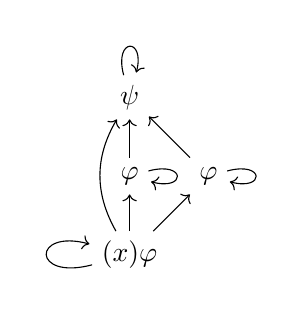
\begin{tikzpicture}[->]
			\node (1) {\((x) \varphi\)};
			\node (2) [above of = 1] {\(\varphi\)};
			\node (3) [right of=2] {\(\varphi\)};
			\node (4) [above of =2] {\(\psi\)};
			\path
			(1) edge node {} (2)
			(1) edge [bend left] node {} (4)
			(1) edge node {} (3)
			(2) edge node {} (4)
			(3) edge node {} (4)
			(1) edge [loop left] node {} (1)
			(2) edge [loop right] node {} (2)
			(3) edge [loop right] node {} (3)
			(4) edge [loop above] node {} (4);
		\end{tikzpicture}\\

		\(M \vDash_x X \varphi\), \(M \nvDash_x G \varphi\)\\
		\(M \vDash_x F \varphi\), \(M \vDash_x U(\varphi, \psi)\)\\
		\(M \vDash_x W(\varphi, \psi)\), \(M \vDash_x R(\varphi, \psi)\)
	\end{center}
\end{example}
\newpage
\begin{example}
consideriamo la relazione:
	\begin{center}
		\((S,R)\) : 
		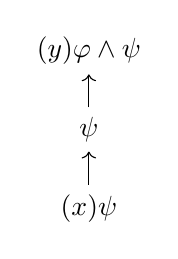
\begin{tikzpicture}[->]
			\node (1) {\((x) \psi\)};
			\node (2) [above of=1] {\(\psi\)};
			\node (3) [above of=2] {\((y) \varphi \land \psi\)};
			\path
			(1) edge node {} (2)
			(2) edge node {} (3);
		\end{tikzpicture}
		\((S,R^*)\):
	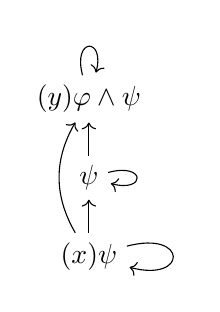
\begin{tikzpicture}[->]
		\node (1) {\((x) \psi\)};
		\node (2) [above of=1] {\(\psi\)};
		\node (3) [above of=2] {\((y) \varphi \land \psi\)};
		\path
		(1) edge node {} (2)
		(1) edge [bend left] node {} (3)
		(2) edge node {} (3)
		(1) edge [loop right] node {} (1)
		(2) edge [loop right] node {} (2)
		(3) edge [loop above] node {} (3);
	\end{tikzpicture}\\
	\(M \vDash_x X \psi\), \(M \vDash_x G \psi\), \(M \vDash_y G \psi\)\\
	\(M \nvDash_x X \varphi\), \(M \nvDash_x G \varphi\), \(M \vDash_y G \varphi\)\\
	\(M \vDash_x F \varphi\), \(M \vDash_x U(\psi, \varphi)\)\\
	\(M \vDash_x W(\psi, \varphi)\), \(M \vDash_x R(\varphi, \psi)\)
	\end{center}
	\(\varphi R \psi : \neg U(\neg \varphi, \neg \psi)\).\\
	\(M vDash_x \neg U(\neg \varphi, \neg \psi) \iff \)\\
	\(M \nvDash_x U(\neg \varphi, \neg \psi) \iff \)\\
	o \(\forall z \in S | (x,z) \in R^*, M \vDash_z \psi\)\\
	o \(\forall z \in S | (x,z) \in R^*. M \vDash_z \neg \psi, \exists y \in S | (x,y) \in R^*, (x,z) \in R^*, y \neq z, M \vDash_y \varphi\)\\
	\(\psi\) deve essere vere fino al punto in cui inzia ad essere vera \(\varphi\) (\(\varphi\) rilascia \(\psi\))
\end{example}
\newpage
\subsubsection{logiche temporali CTL (Computation Tree Logic)}
In queste logiche modali, quantifichiamo sui cammini del grafo diretto\\
che rappresenta il frame \((S,R)\).\\
I connettivi modali sono:
\begin{center}
	\(AX, EX, AF, EF, AG, EG\) (1-ari)\\
	\(AU, EU\) (2-ari)
\end{center}
A sta per "Along all paths"\\
E sta per "along at least one path (there Exists)"\\
\textbf{Semantica:}
\begin{enumerate}
	\item \(M \vDash_w AX \psi \) se e solo se \(\forall v \in S | (w,s) \in R \text{(c'è un arco)} , M \vDash_s \psi\),\\
	 		ossia si comporta come \(\Box\) su \((S,R)\)
	\item \(M \vDash_w EX \psi \) se e solo se \(\exists s \in S | (w,s) \in R \text{(c'è un arco)} , M \vDash_s \psi\),\\
	 		ossia si comporta come \(\Diamond\) su \((S,R)\)
	\item \(AG\) si comporta come \(\Box\) su \((S,R^*)\)
	\item \(M \vDash_w EG \varphi\) se e solo se esiste un cammino in \((S,R)\) tale che \(M \vDash_{s_i} \varphi\)\\
			(lungo il cammino)
	\item \(M \vDash_w EU (\varphi, \psi)\) se e solo se esiste un cammino in \((S,R)\) tale che \(M \vDash_{s_i} U(\varphi, \psi)\)\\
			(lungo il cammino, possiamo intenderlo come sotto-frame)
\end{enumerate}
Analogamente si definiscono gli altri connettivi modali.
\begin{example}
	nei grafi:
	\begin{center}
        \begin{tikzpicture}[->]
          \node (1) {\((S_0)\circ\)};
          \node (2) [below of=1] {\(\circ\)};
          \node (3) [right of =2] {\(\circ\)};
          \node (4) [below of=2] {\(\circ\)};
          \node (5) [right of = 4] {\(\varphi\)};
          \node (6) [right of = 5] {\(\varphi\)};
		  \node (7) [right of = 6] {\(\varphi\)};
		  \node (8) [below of=4]{\(\varphi\)};
          \node (9) [right of = 8] {\(\circ\)};
          \node (10) [right of = 9] {\(\circ\)};
          \node (11) [right of = 10] {\(\circ\)};
          \node (12) [right of = 11] {\(\circ\)};
          \node (13) [below of=8] {\(\circ\)};
		  \node (14) [below of=9] {\(\varphi\)};
		  \node (15) [below of=14] {\(\circ\)};

		  \path
			(1) edge node {} (2)
			(1) edge node {} (3)
			(2) edge node {} (4)
			(3) edge node {} (5)
			(3) edge node {} (6)
			(3) edge node {} (7)
			(4) edge node {} (8)
			(4) edge node {} (9)
			(5) edge node {} (10)
			(6) edge node {} (11)
			(7) edge node {} (12)
			(8) edge node {} (13)
			(9) edge node {} (14)
			(14) edge node {} (15);

        \end{tikzpicture}
		\(M \vDash_{S_0} AF \varphi\)
        \begin{tikzpicture}[->]
          \node (1) {\((S_0)\circ\)};
          \node (2) [below of=1] {\(\circ\)};
          \node (3) [right of =2] {\(\circ\)};
          \node (4) [below of=2] {\(\circ\)};
          \node (5) [right of = 4] {\(\circ\)};
          \node (6) [right of = 5] {\(\circ\)};
		  \node (7) [right of = 6] {\(\circ\)};
		  \node (8) [below of=4]{\(\circ\)};
          \node (9) [right of = 8] {\(\varphi\)};
          \node (10) [right of = 9] {\(\circ\)};
          \node (11) [right of = 10] {\(\circ\)};
          \node (12) [right of = 11] {\(\circ\)};
          \node (13) [below of=8] {\(\circ\)};
		  \node (14) [below of=9] {\(\circ\)};
		  \node (15) [below of=14] {\(\circ\)};

		  \path
			(1) edge node {} (2)
			(1) edge node {} (3)
			(2) edge node {} (4)
			(3) edge node {} (5)
			(3) edge node {} (6)
			(3) edge node {} (7)
			(4) edge node {} (8)
			(4) edge node {} (9)
			(5) edge node {} (10)
			(6) edge node {} (11)
			(7) edge node {} (12)
			(8) edge node {} (13)
			(9) edge node {} (14)
			(14) edge node {} (15);

        \end{tikzpicture}
		\(M \vDash_{S_0} EF \varphi\)\\
		\begin{tikzpicture}[->]
			\node (1) {\((S_0)\varphi\)};
			\node (2) [below of=1] {\(\varphi\)};
			\node (3) [right of =2] {\(\varphi\)};
			\node (4) [below of=2] {\(\varphi\)};
			\node (5) [right of = 4] {\(\varphi\)};
			\node (6) [right of = 5] {\(\varphi\)};
			\node (7) [right of = 6] {\(\varphi\)};
			\node (8) [below of=4]{\(\varphi\)};
			\node (9) [right of = 8] {\(\varphi\)};
			\node (10) [right of = 9] {\(\varphi\)};
			\node (11) [right of = 10] {\(\varphi\)};
			\node (12) [right of = 11] {\(\varphi\)};
			\node (13) [below of=8] {\(\varphi\)};
			\node (14) [below of=9] {\(\varphi\)};
			\node (15) [below of=14] {\(\varphi\)};
  
			\path
			  (1) edge node {} (2)
			  (1) edge node {} (3)
			  (2) edge node {} (4)
			  (3) edge node {} (5)
			  (3) edge node {} (6)
			  (3) edge node {} (7)
			  (4) edge node {} (8)
			  (4) edge node {} (9)
			  (5) edge node {} (10)
			  (6) edge node {} (11)
			  (7) edge node {} (12)
			  (8) edge node {} (13)
			  (9) edge node {} (14)
			  (14) edge node {} (15);
  
		  \end{tikzpicture}
		  \(M \vDash_{S_0} AG \varphi\)\\
    \end{center}
\end{example}
\newpage
\subsubsection{logiche CTL*}
Le logiche CTL* hanno la stessa semantica delle LTL, a cui aggiungiamo i quantificatori\\
\(A\) "Along all paths"\\
\(E\) "Along at least one path".\\
Quindi CTL* contiene LTL e CTL.\\
In LTL possiamo esprimere l'affermazione "su tutti i cammini in cui appare \(\psi\) appare anche \(\varphi\)":
\begin{center}
	\(F\varphi \implies F \psi\)
\end{center}
in CTL non possiamo esprimerla, ma in CTL* si, dato che contiene LTL.\\
\begin{center}
	\(E(GF\varphi)\)
\end{center}
ovviamente tale affermazione non è esprimibile in LTL a meno che il frame \((S,R)\) non abbia un solo cammino.\\
Non è esprimibile neanche in CTL; infatti ha un altro significato:
\begin{example} in CTL:\\
	\begin{center}
        \begin{tikzpicture}[->]
			\node (1) {\((S_0)\varphi\)};
			\node (2) [below of=1] {\(\circ\)};
			\node (3) [right of =2] {\(\circ\)};
			\node (4) [below of=2] {\(\circ\)};
			\node (5) [right of = 4] {\(\varphi\)};
			\node (6) [right of = 5] {\(\varphi\)};
			\node (7) [right of = 6] {\(\varphi\)};
			\node (8) [below of=4]{\(\varphi\)};
			\node (9) [right of = 8] {\(\circ\)};
			\node (10) [right of = 9] {\(\circ\)};
			\node (11) [right of = 10] {\(\circ\)};
			\node (12) [right of = 11] {\(\circ\)};
			\node (13) [below of=8] {\(\circ\)};
			\node (14) [below of=9] {\(\varphi\)};
			\node (15) [below of=14] {\(\circ\)};
  
			\path
			  (1) edge node {} (2)
			  (1) edge node {} (3)
			  (2) edge node {} (4)
			  (3) edge node {} (5)
			  (3) edge node {} (6)
			  (3) edge node {} (7)
			  (4) edge node {} (8)
			  (4) edge node {} (9)
			  (5) edge node {} (10)
			  (6) edge node {} (11)
			  (7) edge node {} (12)
			  (8) edge node {} (13)
			  (9) edge node {} (14)
			  (14) edge node {} (15);
  
		  \end{tikzpicture}\\
		  \(M \vDash_{S_0} EG(EF \varphi)\)
	\end{center}
\end{example}
\newpage
\subsection{Model checking}
\begin{example}
	Quando più processi eseguono in contemporanea, se condividono una risorsa\\
	potrebbe essere necessario assicurare che non vi accedano nello stesso momento.\\
	Ad esempio non vorremmo che più di un provesso modifichi un file nello stesso momento.\\
	Definiamo delle "sezioni critiche" per ogni codice del processo e le disponiamo\\
	in modo che due processi non si trovino nella stessa sezione critica nello stesso momento.\\
	vogliamo che valga la seguente proprietà:
	\begin{center}
		Sicurezza: "Un processo alla volta può stare nella sezione critica"
	\end{center}
	per due processi P1 e P2, consideriamo le variabili:
	\begin{itemize}
		\item \(n_1 = \) "processo 1 non sta in stato critico"
		\item \(n_2 = \) "processo 2 non sta in stato critico"
		\item \(c_1 = \) "processo 1 sta in stato critico"
		\item \(c_2 = \) "processo 2 sta in stato critico"
		\item \(t_1 = \) "processo 1 prova a entrare in stato critico"
		\item \(t_2 = \) "processo 2 prova a entrare in stato critico"
	\end{itemize}

	Sicurezza è espriminile in LTL come: \(\varphi_1 = G\neg (c_1 \land c_2)\)\\
	ossia \(M \vDash_{S_0} G\neg (c_1 \land c_2)\)\\
	un'altra condizione che vogliamo sia verificata è:
	\begin{center}
		Vitalità : "Ogni volta che un processo chiede di entrare nella sua sezione critica, gli sarà permesso in un altro memento"	
	\end{center}
	Questa condizione è esprimibile in CTL come:\\
	\(M \vDash_{S_0} (AGt_1 \implies EF c_1) \land (AGt_2 \implies EF c_2) \equiv \varphi_2\)\\
	considerando il seguente frame:
	\begin{center}
		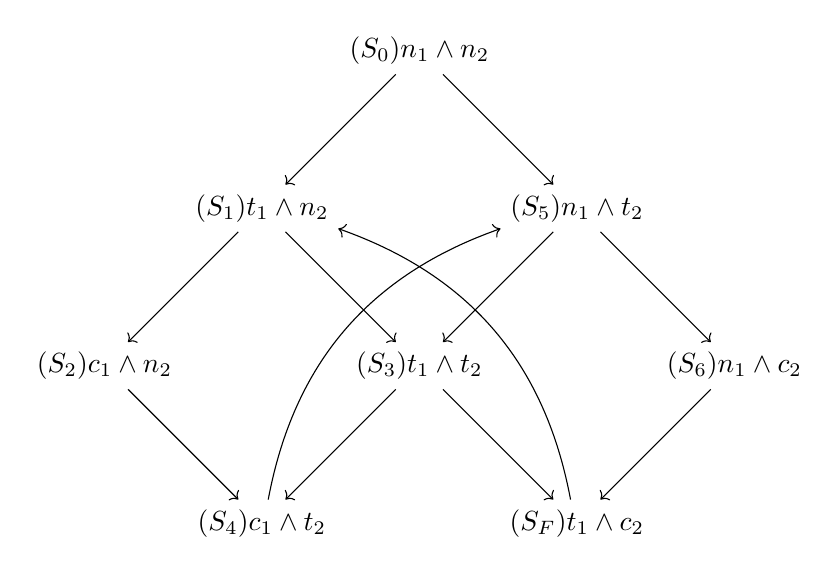
\begin{tikzpicture}[->, node distance=2cm]
			\node (1) {\((S_0) n_1 \land n_2\)};
			\node (2) [below of=1, left of=1] {\((S_1) t_1 \land n_2\)};
			\node (3) [below of = 1, right of =1] {\((S_5) n_1 \land t_2\)};
			\node (4) [below of=2, left of =2] {\((S_2) c_1 \land n_2\)};
			\node (5) [below of =2, right of = 2] {\((S_3) t_1 \land t_2\)};
			\node (6) [below of=3, right of = 3] {\((S_6) n_1 \land c_2\)};
			\node (7) [below of =4, right of = 4] {\((S_4) c_1 \land t_2\)};
			\node (8) [below of=5, right of=5]{\((S_F) t_1 \land c_2\)};

			\path
			  (1) edge node {} (2)
			  (1) edge node {} (3)
			  (2) edge node {} (4)
			  (2) edge node {} (5)
			  (3) edge node {} (5)
			  (3) edge node {} (6)
			  (4) edge node {} (7)
			  (5) edge node {} (7)
			  (5) edge node {} (8)
			  (6) edge node {} (8)
			  (7) edge[bend left] node {} (3)
			  (8) edge [bend right] node {} (2);

		  \end{tikzpicture}\\
		abbiamo che vale \(M \vDash_{S_0} \varphi_1 \land \varphi_2\)
	\end{center}
\end{example}
Esistono algoritmi per verificare validità di tali formule in CTL*.\\
Un famoso model-checker è NuSMV (new symbolic model verifier)\\
mantenuto dalla fondazione Bruno Kessler.\\
vedi anche il libro \textit{"Logic in computer science"} di Huth e Ryan.
\begin{center}
	\href{https://nusmv.fbk.eu}{vai al sito}\\
\end{center}

\end{document}